\documentclass[11pt,a4paper]{report}

% ---------- PACCHETTI ----------
\usepackage[utf8]{inputenc}
\usepackage[T1]{fontenc}
\usepackage[italian]{babel}
\usepackage{amsmath,amssymb}
\usepackage{cancel}
\usepackage{circuitikz}
\usepackage{tikz}
\usetikzlibrary{arrows.meta,calc,positioning}
\usepackage{booktabs}
\usepackage{array}
\usepackage{geometry}
\usepackage[table]{xcolor}
\usepackage{textcomp}
\usepackage{enumitem}
\usepackage{adjustbox}
\usepackage{fancyhdr}
\usepackage{titlesec}
\usepackage{siunitx}
\usepackage[colorlinks=true,linkcolor=noteblue,citecolor=noteblue,urlcolor=noteblue,bookmarks=true,bookmarksopen=true]{hyperref}
\usepackage{ccicons}

\geometry{margin=2.5cm}
\setlength{\headheight}{14pt}
\ctikzset{resistors/scale=0.7, transistors/scale=0.8, logic ports/scale=0.8}

% ---------- COLORI ----------
\definecolor{noteblue}{RGB}{0,70,140}
\definecolor{noteteal}{RGB}{0,128,128}
\definecolor{notered}{RGB}{180,0,0}
\definecolor{notedarkred}{RGB}{120,0,0}

% ---------- INTESTAZIONI ----------
\pagestyle{fancy}
\fancyhf{}
\fancyhead[L]{Elettronica Digitale -- Appunti}
\fancyhead[R]{\thepage}
\renewcommand{\headrulewidth}{0.4pt}

\titleformat{\chapter}[hang]{\Large\bfseries\color{notered}}{Capitolo \thechapter.}{0.5em}{}
\titleformat{\section}{\large\bfseries\color{black}}{\thesection}{0.5em}{}

% ---------- COMANDI UTILI ----------
\newcommand{\defbox}[1]{%
  \par\medskip
  \noindent\fbox{%
    \begin{minipage}{\dimexpr\linewidth-2\fboxsep-2\fboxrule\relax}%
      \sloppy
      #1%
    \end{minipage}%
  }%
  \par\medskip
}

\newenvironment{fitcenter}{%
  \begin{center}%
  \begin{adjustbox}{max width=\linewidth}%
}{%
  \end{adjustbox}%
  \end{center}%
}

\title{\color{notered}\textbf{Elettronica Digitale}\\[0.3em]\large Appunti}
\author{}
\date{}

\begin{document}

% Custom title page inspired by the provided image
\begin{titlepage}
  \centering
  \vspace*{0.8cm}
  {\Large\scshape\color{notedarkred}APPUNTI DI\par}
  \vspace{0.6cm}
  {\Huge\bfseries\color{notered}\MakeUppercase{Elettronica Digitale}\par}
  \vspace{0.8cm}
  {\color{notered}\rule{8cm}{1.2pt}\par}
  \vspace{1.2cm}
  {\Large\scshape Giosu\`e Aiello\par}
  \vfill
  \noindent
  \begin{minipage}[b]{0.5\linewidth}
    \textit{versione 1.0}
  \end{minipage}%
  \begin{minipage}[b]{0.5\linewidth}
    \raggedleft
    Universit\`a di Pisa\\
    anno 2025--2026
  \end{minipage}
  \thispagestyle{empty}
\end{titlepage}

\vspace*{\fill}
\noindent {\Large \ccbync} Licensed under Creative Commons Attribution-NonCommercial 4.0 International. \\ To view a copy of this license, visit \url{https://creativecommons.org/licenses/by-nc/4.0/}.
\newpage

% Make the Table of Contents use black links (not all red)
{\hypersetup{linkcolor=black}
\pdfbookmark[0]{Indice}{indice}
\tableofcontents
\newpage}

% ======================================================================
\chapter{Segnali, algebra di Boole e reti logiche}
\textit{(27 febbraio -- 2 marzo 2026)}

\section{Segnali analogici e digitali}

\defbox{
\textbf{Segnale analogico}: assume valori continui (onde). È il tipo di segnale presente in natura.\\[0.3em]
\textbf{Segnale digitale}: assume valori discreti, tipicamente $\{0,1\}$.
}

Il passaggio da un segnale analogico a uno digitale permette di \textbf{memorizzare meglio i dati}: un valore discreto è notevolmente più robusto al rumore, non subisce degrado nel tempo, ed è molto più semplice da elaborare e conservare in dispositivi di memoria rispetto a un segnale continuo. Inoltre, i sistemi digitali garantiscono una \textbf{riproducibilità esatta} dei risultati e godono di un'elevata flessibilità grazie alla possibilità di essere programmati via software.

\section{Algebra di Boole}

L'algebra di Boole fu pubblicata a metà dell'Ottocento (nel 1854, ad opera del matematico inglese George Boole, con il trattato \emph{An Investigation of the Laws of Thought}) come base matematica per lo studio della logica. Per definirla formalmente servono i seguenti ingredienti:

\begin{itemize}[leftmargin=1.5em]
    \item un insieme $B$ che contiene \textbf{2 valori} (es. $\{0,1\}$);
    \item su $B$ agiscono \textbf{2 operazioni} (tipicamente $+$ e $\cdot$, cioè OR e AND);
    \item gli \textbf{elementi neutri} delle due operazioni sono gli stessi 2 elementi di $B$;
    \item si definisce un'ulteriore operazione, il \textbf{NOT}, che manda i due valori l'uno nell'altro ($0\to1$, $1\to0$).
\end{itemize}

\textit{Notazione}: la negazione di una variabile si indica con un trattino sopra la lettera, ad esempio $\overline{A}$.

\subsection{Il concetto di duale}

\defbox{\textbf{Duale} di un'espressione booleana: si ottiene scambiando tra loro le due operazioni principali e gli elementi neutri:
\begin{itemize}[leftmargin=1.3em]
    \item $+$ con $\cdot$;
    \item $0$ con $1$;
    \item il NOT resta invariato.
\end{itemize}
Quindi, se una proprietà è vera, anche la sua forma duale è vera.}

\noindent Per esempio, il duale di
\[
A + 0 = A
\]
\`e
\[
A \cdot 1 = A.
\]

\noindent Allo stesso modo, il duale della proprietà di complementarità
\[
A + \overline{A} = 1
\]
\`e
\[
A \cdot \overline{A} = 0.
\]

\noindent Il \textbf{principio di dualità} è molto utile perché, una volta nota una proprietà, si ottiene immediatamente la sua versione duale senza doverla dimostrare separatamente. Ad esempio:
\begin{itemize}[leftmargin=1.5em]
    \item commutativa: $A+B=B+A$ ha come duale $A\cdot B=B\cdot A$;
    \item associativa: $(A+B)+C=A+(B+C)$ ha come duale $(A\cdot B)\cdot C=A\cdot(B\cdot C)$;
    \item distributiva: $A+(B\cdot C)=(A+B)\cdot(A+C)$ ha come duale $A\cdot(B+C)=(A\cdot B)+(A\cdot C)$.
\end{itemize}

\section{Cenni storici}

\begin{itemize}[leftmargin=1.5em]
    \item Nel 1938 \textbf{Claude Shannon} introdusse l'uso dell'algebra di Boole per l'analisi e la sintesi dei circuiti a relè, inventando di fatto l'applicazione alle reti logiche.
    \item \textbf{Huntington} (1904) formulò i famosi postulati che definiscono rigorosamente l'algebra booleana e dimostrò che ogni rete logica può essere implementata usando solo porte elementari.
    \item Il \textbf{transistor} (\emph{transfer} + \emph{resistor}) fu inventato nel 1947 ai Bell Labs. Da lì, nel giro di circa dieci anni, nacque l'elettronica a stato solido moderna e nel 1958 fu realizzato il primo circuito integrato.
\end{itemize}

\section{Reti logiche}

Una rete logica può essere vista come una scatola nera con $n$ ingressi $I_i$ e $m$ uscite $O_i$:

\begin{center}
\begin{circuitikz}
\draw (0,0) rectangle (2.4,2.2);
\node at (1.2,1.1) {rete logica};
\foreach \y in {1.8,1.4,1.0,0.6}{
  \draw[-latex] (-1.1,\y) -- (0,\y);
}
\node[left] at (-1.1,2.1) {$n$ entrate};
\node[left,yshift=-0.3cm] at (-1.1,1.0) {$I_i$};
\draw[-latex] (2.4,1.6) -- (3.5,1.6);
\draw[-latex] (2.4,0.9) -- (3.5,0.9);
\node[right] at (3.5,2.1) {$m$ uscite};
\node[right,yshift=-0.3cm] at (3.5,1.25) {$O_i$};
\end{circuitikz}
\end{center}

\defbox{
$O_i = f(I_i)$: per ogni uscita esiste una funzione che dipende dagli ingressi $I_i$; tale funzione è \textbf{suriettiva}. Sia gli $O_i$ che gli $I_i$ possono assumere solo i valori $0$ oppure $1$.
}

\subsection{Funzioni a 1 ingresso}

Con un solo ingresso $I$ esistono $2^{2^1}=4$ possibili funzioni di uscita:

\begin{center}
\begin{tabular}{c|cccc}
\toprule
$I$ & $O_1$ & $O_2$ & $O_3$ & $O_4$\\
\midrule
0 & 0 & 1 & 0 & 1\\
1 & 0 & 0 & 1 & 1\\
\midrule
 & \footnotesize 0 & \footnotesize NOT & \footnotesize ID & \footnotesize 1\\
\bottomrule
\end{tabular}
\end{center}

Questa è la \textbf{tabella di verità} delle 4 funzioni a un ingresso: due sono costanti ($0$ e $1$), una è l'\textbf{identità} (ID, o \emph{buffer}) e una è la \textbf{negazione} (NOT).

\begin{center}
\begin{circuitikz}
\node[buffer port] (b1) at (0,0) {};
\draw (b1.in 1) -- ++(-0.6,0);
\draw (b1.out) -- ++(0.6,0);
\node[below=0.3cm] at (b1) {ID (buffer)};

\node[not port] (n1) at (5,0) {};
\draw (n1.in 1) -- ++(-0.6,0);
\draw (n1.out) -- ++(0.6,0);
\node[below=0.3cm] at (n1) {NOT};
\end{circuitikz}
\end{center}

\subsection{Funzioni a 2 ingressi}

Con due ingressi $I_1, I_0$ ci sono $2^2=4$ combinazioni in ingresso e $2^{2^2}=16$ possibili funzioni di uscita. La tabella completa è:

\begin{fitcenter}
\small
\begin{tabular}{c|cccc|l|l}
\toprule
\textbf{Funzione} & \textbf{00} & \textbf{01} & \textbf{10} & \textbf{11} & \textbf{Espressione Booleana} & \textbf{Nome comune / Significato} \\
\midrule
$O_1$    & 0 & 0 & 0 & 0 & $0$ & Costante 0 (Falsa) \\
$O_2$    & 1 & 0 & 0 & 0 & $\overline{I_1 + I_0} = \overline{I_1} \cdot \overline{I_0}$ & \textbf{NOR} \\
$O_3$    & 0 & 1 & 0 & 0 & $\overline{I_1} \cdot I_0$ & Inibizione di $I_1$ (da $I_0$) \\
$O_4$    & 0 & 0 & 1 & 0 & $I_1 \cdot \overline{I_0}$ & Inibizione di $I_0$ (da $I_1$) \\
$O_5$    & 0 & 0 & 0 & 1 & $I_1 \cdot I_0$ & \textbf{AND} \\
$O_6$    & 1 & 1 & 0 & 0 & $\overline{I_1}$ & \textbf{NOT} $I_1$ \\
$O_7$    & 1 & 0 & 1 & 0 & $\overline{I_0}$ & \textbf{NOT} $I_0$ \\
$O_8$    & 1 & 0 & 0 & 1 & $\overline{I_1 \oplus I_0} = I_1 \odot I_0$ & \textbf{XNOR} (Equivalenza) \\
$O_9$    & 0 & 1 & 1 & 0 & $I_1 \oplus I_0$ & \textbf{XOR} (OR esclusivo) \\
$O_{10}$ & 0 & 1 & 0 & 1 & $I_0$ & Identità $I_0$ (Buffer $I_0$) \\
$O_{11}$ & 0 & 0 & 1 & 1 & $I_1$ & Identità $I_1$ (Buffer $I_1$) \\
$O_{12}$ & 1 & 1 & 1 & 0 & $\overline{I_1 \cdot I_0}$ & \textbf{NAND} \\
$O_{13}$ & 1 & 1 & 0 & 1 & $I_1 + \overline{I_0}$ o $I_0 \rightarrow I_1$ & Implicazione ($I_0 \implies I_1$) \\
$O_{14}$ & 0 & 1 & 1 & 1 & $I_1 + I_0$ & \textbf{OR} \\
$O_{15}$ & 1 & 0 & 1 & 1 & $\overline{I_1} + I_0$ o $I_1 \rightarrow I_0$ & Implicazione ($I_1 \implies I_0$) \\
$O_{16}$ & 1 & 1 & 1 & 1 & $1$ & Costante 1 (Vera) \\
\bottomrule
\end{tabular}
\end{fitcenter}

\noindent\footnotesize \textit{Nota sui simboli}: 
L'operatore $\oplus$ (più cerchiato) rappresenta lo \textbf{XOR} (OR esclusivo, $I_1 \oplus I_0$), che vale 1 se e solo se i due ingressi sono diversi. 
L'operatore $\odot$ (punto cerchiato) rappresenta lo \textbf{XNOR} (equivalenza logica, $I_1 \odot I_0 = \overline{I_1 \oplus I_0}$), che vale 1 se e solo se i due ingressi sono uguali.

\noindent Tra le 16 funzioni, le più importanti hanno un nome ed un simbolo proprio:

\begin{fitcenter}
\begin{circuitikz}
\node[and port] (g1) at (0,0) {};
\draw (g1.in 1) -- ++(-0.5,0); \draw (g1.in 2) -- ++(-0.5,0); \draw (g1.out) -- ++(0.5,0);
\node[below=0.3cm] at (g1) {AND};

\node[or port] (g2) at (3,0) {};
\draw (g2.in 1) -- ++(-0.5,0); \draw (g2.in 2) -- ++(-0.5,0); \draw (g2.out) -- ++(0.5,0);
\node[below=0.3cm] at (g2) {OR};

\node[nand port] (g3) at (6,0) {};
\draw (g3.in 1) -- ++(-0.5,0); \draw (g3.in 2) -- ++(-0.5,0); \draw (g3.out) -- ++(0.5,0);
\node[below=0.3cm] at (g3) {NAND};

\node[nor port] (g4) at (9,0) {};
\draw (g4.in 1) -- ++(-0.5,0); \draw (g4.in 2) -- ++(-0.5,0); \draw (g4.out) -- ++(0.5,0);
\node[below=0.3cm] at (g4) {NOR};

\node[xor port] (g5) at (12,0) {};
\draw (g5.in 1) -- ++(-0.5,0); \draw (g5.in 2) -- ++(-0.5,0); \draw (g5.out) -- ++(0.5,0);
\node[below=0.3cm] at (g5) {XOR (OR escl.)};
\end{circuitikz}
\end{fitcenter}

\subsection{Funzioni a $n$ ingressi}

In generale, con $n$ ingressi si hanno $2^n$ possibili combinazioni in ingresso e $2^{2^n}$ possibili funzioni di uscita. Le porte AND, NAND, OR, NOR, XOR si generalizzano naturalmente a $n$ ingressi.

\section{Bit di parità}

\defbox{
Il \textbf{bit di parità} è un bit aggiuntivo utilizzato per rilevare errori singoli che possono verificarsi quando un segnale viene trasmesso in un canale rumoroso:
\begin{itemize}[leftmargin=1.3em]
    \item Nella \textbf{parità pari} (\emph{even parity}), il bit $P$ si sceglie affinché il numero totale di ``1'' trasmessi sia pari:
    \begin{itemize}
        \item se il numero di $1$ nel dato è \textbf{pari} $\Rightarrow P = 0$;
        \item se il numero di $1$ nel dato è \textbf{dispari} $\Rightarrow P = 1$.
    \end{itemize}
    \item Nella \textbf{parità dispari} (\emph{odd parity}), la regola è invertita (il numero totale di ``1'' deve essere dispari).
\end{itemize}
Il controllo di parità è semplice ma limitato: può rilevare un numero dispari di errori (tipicamente un solo bit errato), ma fallisce se avvengono due errori simultanei, poiché la parità complessiva rimane inalterata.
}

\medskip
\noindent\textbf{Esempio numerico.} Supponiamo di trasmettere il dato a 3 bit $D = 110$ usando \textbf{parità pari}:
\begin{itemize}[leftmargin=1.5em]
    \item Il dato $110$ contiene \textbf{due} $1$ $\Rightarrow$ il numero di $1$ è già pari $\Rightarrow P = 0$.
    \item Si trasmette la sequenza $\underbrace{1\;1\;0}_{\text{dato}}\underbrace{0}_{P}$ (totale: due $1$, pari $\checkmark$).
    \item Se durante la trasmissione un bit si corrompe, ad es.\ arriva $\mathbf{1\;0\;0\;0}$: ora c'è solo un $1$, il numero è \textbf{dispari} $\Rightarrow$ errore rilevato!
    \item Se invece si corrompono \textbf{due} bit contemporaneamente, la parità resta pari e l'errore \textbf{non} viene rilevato (limite del metodo).
\end{itemize}

\section{Esercizio: semplice circuito per abilitare la presa dati}

\textit{Disegnare un circuito che generi un segnale per abilitare la presa dati di un esperimento se ha il segnale di \textbf{sicurezza} S attivo, se c'è la richiesta di una presa dati che può essere di \textbf{calibrazione} o \textbf{standard} (non entrambe), e se l'operatore chiede di abilitare l'\textbf{acquisizione}. Inoltre la presa dati si deve arrestare se S non è più attivo.}

\medskip
\noindent\textbf{Come si risolve (ragionamento passo per passo):}

\begin{enumerate}[leftmargin=1.5em]
    \item \textbf{Identificare le condizioni.} L'uscita deve essere $1$ (abilitata) \emph{solo} quando \textbf{tutte} le seguenti condizioni sono soddisfatte:
    \begin{itemize}
        \item il segnale di sicurezza $S = 1$;
        \item il segnale di acquisizione $A = 1$;
        \item esattamente \textbf{uno} tra calibrazione $C$ e standard $T$ è attivo (non né entrambi, né nessuno).
    \end{itemize}
    \item \textbf{Tradurre ogni condizione in logica:}
    \begin{itemize}
        \item ``Sicurezza attiva'' $\rightarrow$ basta $S$.
        \item ``Acquisizione attiva'' $\rightarrow$ basta $A$.
        \item ``Calibrazione \emph{o} Standard, ma \textbf{non entrambe}'' $\rightarrow$ questa è esattamente la definizione dello \textbf{XOR}: $C \oplus T$ vale $1$ quando i due ingressi sono \emph{diversi} (uno $0$ e uno $1$), e $0$ quando sono uguali (entrambi $0$ oppure entrambi $1$).
    \end{itemize}
    \item \textbf{Combinare le condizioni con AND:} poiché tutte e tre le condizioni devono essere vere \emph{contemporaneamente}, si mettono in AND:
    \[
        \text{Uscita} = S \cdot A \cdot (C \oplus T)
    \]
    \item \textbf{Ordine delle porte:} si mette $S$ nell'ultima porta AND così, quando il segnale di sicurezza si abbassa, l'uscita si spegne immediatamente (minimo ritardo di propagazione).
\end{enumerate}

\begin{center}
\begin{circuitikz}[scale=0.9, every node/.style={scale=0.9}]
\node[xor port] (x1) at (0,0) {};
\draw (x1.in 1) -- ++(-1.2,0) node[left]{Calibrazione ($C$)};
\draw (x1.in 2) -- ++(-1.2,0) node[left]{Standard ($T$)};

\node[and port] (a1) at (2.6,0.4) {};
\draw (x1.out) -- (a1.in 1);
\draw (a1.in 2) -- ++(-1.2,-1.6) node[left]{Acquisizione ($A$)};

\node[and port] (a2) at (5.2,0.9) {};
\draw (a1.out) -- (a2.in 2);
\draw (a2.in 1) -- ++(-2.4,1.2) node[left]{Sicurezza ($S$)};

\draw (a2.out) -- ++(0.8,0) node[right]{Uscita};
\end{circuitikz}
\end{center}

\noindent\textbf{Verifica con un esempio:} supponiamo $S=1$, $A=1$, $C=1$, $T=0$.
\[
    C \oplus T = 1 \oplus 0 = 1, \qquad \text{Uscita} = 1 \cdot 1 \cdot 1 = 1 \quad \checkmark
\]
Se invece sia calibrazione che standard sono attivi ($C=1$, $T=1$): $C \oplus T = 0 \Rightarrow$ Uscita $= 0$ (corretto: le due richieste si escludono a vicenda).

% ======================================================================
\chapter{Realizzazione fisica delle porte logiche}
\textit{(6 marzo 2026)}

\section{Esercizio: bit di parità a 4 bit}

\textit{Progettare un circuito che calcoli il bit di parità di un numero a 4 bit. Il bit di parità è 0 se il numero di 1 nel numero è pari, 1 se è dispari.}

\medskip
\noindent\textbf{Come si risolve (ragionamento passo per passo):}

\begin{enumerate}[leftmargin=1.5em]
    \item \textbf{Capire cosa serve (e perché può sembrare invertita).}
    L'obiettivo della \textbf{parità pari} è che il numero \emph{totale} di $1$ trasmessi (dato $+$ bit $P$) sia sempre \textbf{pari}. Di conseguenza:
    \begin{itemize}
        \item se nel dato ci sono già un numero \textbf{pari} di $1$ $\Rightarrow$ non serve aggiungere nulla $\Rightarrow P = 0$;
        \item se nel dato ci sono un numero \textbf{dispari} di $1$ $\Rightarrow$ bisogna aggiungere un $1$ per bilanciare $\Rightarrow P = 1$.
    \end{itemize}
    \textit{Attenzione}: $P = 1$ \textbf{non} significa ``va tutto bene'', significa ``ho dovuto correggere la parità''. Detto in modo diretto: $P$ vale $1$ quando il conteggio degli $1$ nel dato è \textbf{dispari} (e dunque serviva un $1$ extra per renderlo pari).

    \item \textbf{Riconoscere la porta giusta.} Ricordiamo la tabella dello \textbf{XOR} a 2 ingressi:
    \begin{center}
    \begin{tabular}{cc|c|l}
    \toprule
    $A$ & $B$ & $A \oplus B$ & Significato \\
    \midrule
    0 & 0 & 0 & zero uni $\Rightarrow$ pari \\
    0 & 1 & 1 & un uno $\Rightarrow$ dispari \\
    1 & 0 & 1 & un uno $\Rightarrow$ dispari \\
    1 & 1 & 0 & due uni $\Rightarrow$ pari \\
    \bottomrule
    \end{tabular}
    \end{center}
    Lo XOR vale $1$ esattamente quando il numero di $1$ in ingresso è \textbf{dispari}: è dunque il componente perfetto per calcolare la parità!

    \item \textbf{Estendere a 4 bit con la proprietà associativa.} Lo XOR è \textbf{associativo}, quindi possiamo calcolare la parità su più bit applicandolo in cascata, come somma modulo 2:
    \[
        P = I_3 \oplus I_2 \oplus I_1 \oplus I_0
    \]
    Il risultato vale $1$ se e solo se il numero totale di $1$ tra i 4 bit è dispari (esattamente ciò che vogliamo).

    \item \textbf{Costruire il circuito.} Uno XOR accetta solo 2 ingressi, quindi si procede \textbf{a coppie}:
    \begin{itemize}
        \item Primo livello: $X_A = I_1 \oplus I_0$ e $X_B = I_3 \oplus I_2$ (due porte XOR in parallelo).
        \item Secondo livello: $P = X_A \oplus X_B$ (una porta XOR che combina i risultati parziali).
    \end{itemize}
    Servono quindi \textbf{3 porte XOR} in totale.

    \item \textbf{Verifica numerica.} Prendiamo $N = 1011$:
    \begin{itemize}
        \item Conta degli uni: tre $1$ $\Rightarrow$ dispari $\Rightarrow$ ci aspettiamo $P = 1$.
        \item Calcolo: $X_A = 1 \oplus 1 = 0$, $\quad X_B = 1 \oplus 0 = 1$, $\quad P = 0 \oplus 1 = 1$ \checkmark
    \end{itemize}
    Prendiamo $N = 1100$:
    \begin{itemize}
        \item Conta degli uni: due $1$ $\Rightarrow$ pari $\Rightarrow$ ci aspettiamo $P = 0$.
        \item Calcolo: $X_A = 0 \oplus 0 = 0$, $\quad X_B = 1 \oplus 1 = 0$, $\quad P = 0 \oplus 0 = 0$ \checkmark
    \end{itemize}
\end{enumerate}

\medskip
\noindent Sia $N = I_3 I_2 I_1 I_0$. Si lavora a coppie di bit, applicando lo XOR a multipli di 2:

\begin{center}
\begin{tabular}{cc|c}
\toprule
$I_3$ & $I_2$ & XOR\\
\midrule
0&0&0\\
0&1&1\\
1&0&1\\
1&1&0\\
\bottomrule
\end{tabular}
\qquad
\begin{tabular}{cc|c}
\toprule
$I_1$ & $I_0$ & XOR\\
\midrule
0&0&0\\
0&1&1\\
1&0&1\\
1&1&0\\
\bottomrule
\end{tabular}
\end{center}

Il \textbf{calcolatore di parità} si ottiene combinando in cascata 3 porte XOR:

\begin{center}
\begin{circuitikz}[scale=0.9, every node/.style={scale=0.9}]
\node[xor port] (x1) at (0,1) {};
\draw (x1.in 1) -- ++(-1,0) node[left]{$I_0$};
\draw (x1.in 2) -- ++(-1,0) node[left]{$I_1$};

\node[xor port] (x2) at (0,-1) {};
\draw (x2.in 1) -- ++(-1,0) node[left]{$I_2$};
\draw (x2.in 2) -- ++(-1,0) node[left]{$I_3$};

\node[xor port] (x3) at (2.6,0) {};
\draw (x1.out) -| (x3.in 1);
\draw (x2.out) -| (x3.in 2);
\draw (x3.out) -- ++(0.8,0) node[right]{$P$};
\end{circuitikz}
\end{center}

\section{Verifica di una trasmissione tramite parità}

Calcolando il bit di parità sia alla \textbf{partenza} ($O_1$) che all'\textbf{arrivo} ($O_2$) e confrontandoli con una porta \textbf{XNOR}, si fa passare il segnale solo se $O_1 = O_2$ (cioè $00$ oppure $11$): questo permette di controllare che il segnale non sia stato alterato durante la trasmissione.

\begin{center}
\begin{circuitikz}[scale=0.9, every node/.style={scale=0.9}]
% Block 1: Partenza (Calcolatore di parità)
\draw[thick] (0,0) rectangle (2,1.6);
\node[align=center, font=\small] at (1,0.8) {Calcolatore\\di parità};
\node[above, font=\footnotesize\bfseries] at (1,1.6) {Partenza};

% Input arrows for Block 1
\foreach \y/\label in {1.4/$I_3$, 1.1/$I_2$, 0.8/$I_1$, 0.5/$I_0$} {
  \draw[-latex] (-0.8,\y) -- (0,\y);
  \node[left, font=\scriptsize] at (-0.8,\y) {\label};
}

% XNOR Gate positioned on the right
\node[xnor port] (xn) at (8.6,0.8) {};

% Output of Block 1 (O_1) routed above Block 2 to avoid crossing
\draw[thick] (2,0.8) -- (2.4,0.8) node[above, font=\footnotesize] {$O_1$};
\draw[-latex, thick] (2.4,0.8) -- (2.4,2.2) -- (7.6,2.2) |- (xn.in 1);

% Block 2: Arrivo (Calcolatore di parità)
\draw[thick] (4.2,0) rectangle (6.2,1.6);
\node[align=center, font=\small] at (5.2,0.8) {Calcolatore\\di parità};
\node[above, font=\footnotesize\bfseries] at (5.2,1.6) {Arrivo};

% Input arrows for Block 2 (received bits, possibly with prime)
\foreach \y/\label in {1.4/$I'_3$, 1.1/$I'_2$, 0.8/$I'_1$, 0.5/$I'_0$} {
  \draw[-latex] (3.4,\y) -- (4.2,\y);
  \node[left, font=\scriptsize] at (3.4,\y) {\label};
}

% Output of Block 2 (O_2) routed to XNOR
\draw[thick] (6.2,0.8) -- (6.8,0.8) node[above, font=\footnotesize] {$O_2$};
\draw[-latex, thick] (6.8,0.8) |- (xn.in 2);

% Output of XNOR
\draw (xn.out) -- ++(0.8,0) node[right, align=left, font=\footnotesize] {Abilita se $O_1 = O_2$\\(nessun errore)};
\end{circuitikz}
\end{center}

\section{Caratteristiche fisiche delle porte logiche}

Le diverse \textbf{famiglie logiche} (RTL, DTL, HTL, TTL, ECL, MOS, CMOS) si confrontano in base a parametri come la porta di base, il fan-out, la potenza dissipata, l'immunità al rumore, il ritardo di propagazione e la frequenza massima di funzionamento. In generale:

\begin{itemize}[leftmargin=1.5em]
    \item \textbf{TTL} (Transistor-Transistor Logic): ottimo compromesso velocità/potenza, molto diffusa;
    \item \textbf{ECL} (Emitter-Coupled Logic): velocissima ma con elevato consumo;
    \item \textbf{CMOS} (Complementary Metal-Oxide-Semiconductor): bassissima potenza dissipata, oggi la più usata nei circuiti integrati.
\end{itemize}

\section{Implementazione delle porte logiche}

\subsection{NOT con un singolo transistor}

La porta NOT più semplice si realizza con un singolo transistor NPN in configurazione a emettitore comune, con una resistenza di pull-up $R_C$ verso $V_{CC}$:

\begin{center}
\begin{circuitikz}[american voltages]
\draw (0,0) node[npn](Q1){}
  (Q1.C) to[short,-*] (Q1.C -| 0,2) to[R, l=$R_C$] (Q1.C |- 0,3.5) node[above]{$V_{CC}$}
  (Q1.B) to[short] ++(-1.6,0) node[left]{$V_{in}$}
  (Q1.E) to[short] ++(0,-1) node[ground]{}
  (Q1.C) to[short,-o] ++(1.6,0) node[right]{$V_{out}$}
;
\end{circuitikz}
\end{center}

\defbox{
\begin{itemize}[leftmargin=1.3em]
    \item $V_{in} = 5\,\text{V} \;(=1) \Rightarrow$ il transistor satura $\Rightarrow V_{out} = 0,2\,\text{V} \;(=0)$;
    \item $V_{in} = 0\,\text{V} \;(=0) \Rightarrow$ il transistor è spento $\Rightarrow V_{out} = 5\,\text{V} \;(=1)$.
\end{itemize}
}

\begin{center}
\begin{circuitikz}
\node[not port] (n1) at (0,0) {};
\draw (n1.in 1) -- ++(-0.6,0);
\draw (n1.out) -- ++(0.6,0);
\end{circuitikz}
\end{center}

\subsection{NOT in tecnologia TTL}

Nella tecnologia TTL (\emph{Transistor-Transistor Logic}), la porta logica base non utilizza singoli diodi o resistenze in ingresso, ma sfrutta i transistor bipolari (BJT) per migliorare velocità e prestazioni. La porta NOT TTL standard si divide in tre stadi principali:

\begin{enumerate}[leftmargin=1.5em]
    \item \textbf{Stadio di ingresso}: utilizza un transistor NPN ($Q_1$) in cui l'emettitore funge da ingresso. Se l'ingresso è basso ($0\,\mathrm{V}$), $Q_1$ va in conduzione portando a massa la base dello stadio successivo. Se l'ingresso è alto ($5\,\mathrm{V}$), la giunzione base-emettitore è polarizzata inversamente e la corrente fluisce verso la base del driver.
    \item \textbf{Sfasatore (driver)}: il transistor centrale ($Q_2$) riceve il segnale da $Q_1$ e pilota in controfase i due transistor finali. Produce due segnali logici opposti: uno al collettore e uno all'emettitore.
    \item \textbf{Stadio di uscita a totem-pole}: costituito da due transistor ($Q_3$ e $Q_4$) impilati uno sull'altro e un diodo. Garantisce un'uscita ``forte'' a bassa impedenza in entrambi gli stati logici: $Q_3$ spinge attivamente l'uscita a livello alto (pull-up attivo), mentre $Q_4$ la tira a massa (pull-down). Il diodo serve a garantire che $Q_3$ e $Q_4$ non conducano mai contemporaneamente in fase di transizione.
\end{enumerate}

\begin{center}
\begin{circuitikz}[american voltages, scale=0.85, every node/.style={scale=0.85}]
\draw (0,4.5) -- (7,4.5);
\node[above] at (3.5,4.5) {$V_{CC} \ (+5\,\mathrm{V})$};

% R1
\draw (1,4.5) to[R=$4\,\mathrm{k}\Omega$] (1,2.5) coordinate (bQ1);
% R2
\draw (3.5,4.5) to[R=$1.6\,\mathrm{k}\Omega$] (3.5,2.5) coordinate (cQ2);
% R4
\draw (5.5,4.5) to[R=$130\,\Omega$] (5.5,3.2) coordinate (cQ3);

% Q1
\node[npn] (Q1) at (1.5,1.7) {};
\node at ($(Q1.C)+(0.4,0)$) {$Q_1$};
\draw (bQ1) -| (Q1.B);
\draw (Q1.E) -- ++(-1.5,0) to[short,-o] ++(0,0) node[left]{$V_{in}$};

% Q2
\node[npn] (Q2) at (3.5,1.7) {};
\node at ($(Q2.C)+(0.4,0.1)$) {$Q_2$};
\draw (Q1.C) |- (Q2.B);
\draw (cQ2) -- (Q2.C);

% Q2 emitter resistor
\draw (Q2.E) to[R=$1\,\mathrm{k}\Omega$] ++(0,-1.5) node[ground]{};

% Q3
\node[npn] (Q3) at (5.5,2.4) {};
\node at ($(Q3.C)+(0.4,0)$) {$Q_3$};
\draw (cQ3) -- (Q3.C);
\draw (Q2.C) |- (Q3.B);

% Diode
\draw (Q3.E) to[D] ++(0,-1) coordinate (dout);

% Q4
\node[npn] (Q4) at (5.5,0.6) {};
\node at ($(Q4.C)+(0.4,0)$) {$Q_4$};
\draw (dout) -- (Q4.C);
\draw (Q2.E) |- (Q4.B);
\draw (Q4.E) -- ++(0,-0.3) node[ground]{};

% Vout
\draw (dout) to[short,-o] ++(1.5,0) node[right]{$V_{out}$};

% Labels for stages
\node[align=center, font=\footnotesize, text=blue!80!black] at (1,-0.5) {Stadio di\\ingresso};
\node[align=center, font=\footnotesize, text=blue!80!black] at (3.5,-0.5) {Sfasatore\\(Driver)};
\node[align=center, font=\footnotesize, text=blue!80!black] at (6.2,-0.5) {Uscita a\\Totem-Pole};

% Dashed lines separating stages
\draw[dashed, gray] (2.5, 4.5) -- (2.5, -1);
\draw[dashed, gray] (4.5, 4.5) -- (4.5, -1);

\end{circuitikz}
\end{center}

\section{Immunità al rumore}

L'immunità al rumore di un sistema digitale non è totale, ma è comunque molto più elevata di quella dei sistemi analogici, perché due porte in cascata ``ripuliscono'' il segnale ad ogni passaggio rigenerando i livelli di tensione:

\begin{center}
\begin{circuitikz}
\node[buffer port] (b1) at (0,0) {};
\node[buffer port] (b2) at (2,0) {};
\draw (b1.in 1) -- ++(-0.6,0) node[left]{in};
\draw (b1.out) -- (b2.in 1);
\node[above] at ($(b1.out)!0.5!(b2.in 1)$) {\footnotesize out$'$/in$'$};
\draw (b2.out) -- ++(0.6,0) node[right]{out$''$};
\end{circuitikz}
\end{center}

Per garantire il corretto riconoscimento dei livelli logici, i costruttori definiscono le soglie di tensione per l'ingresso e l'uscita:

\defbox{
\begin{minipage}{0.48\linewidth}
\textbf{Livello alto (High)}
\begin{itemize}[leftmargin=1.3em]
    \item $V_{OH,min}$: $V_{out}$ minima garantita per l'uscita alta;
    \item $V_{OH,max}$: $V_{out}$ massima possibile per l'uscita alta;
    \item $V_{IH,min}$: $V_{in}$ minima richiesta in ingresso per essere letta come alta;
    \item $V_{IH,max}$: $V_{in}$ massima ammessa per un ingresso alto.
\end{itemize}
\end{minipage}
\hfill
\begin{minipage}{0.48\linewidth}
\textbf{Livello basso (Low)}
\begin{itemize}[leftmargin=1.3em]
    \item $V_{OL,min}$: $V_{out}$ minima possibile per l'uscita bassa;
    \item $V_{OL,max}$: $V_{out}$ massima garantita per l'uscita bassa;
    \item $V_{IL,min}$: $V_{in}$ minima ammessa per un ingresso basso;
    \item $V_{IL,max}$: $V_{in}$ massima tollerata in ingresso per essere letta come bassa.
\end{itemize}
\end{minipage}
}

La differenza tra le tensioni garantite in uscita e quelle minime/massime tollerate in ingresso definisce i \textbf{margini di rumore} (\emph{noise margin}):
\[
NM_H = V_{OH,min} - V_{IH,min} \qquad\qquad
NM_L = V_{IL,max} - V_{OL,max}
\]
I margini di rumore ($NM_H$ e $NM_L$) rappresentano l'ampiezza massima di un disturbo (rumore elettrico, fluttuazioni) che può sommarsi al segnale durante il tragitto lungo il filo senza far sì che la porta successiva lo interpreti in modo errato o lo collochi nella \emph{zona proibita}. In altre parole, è il ``cuscinetto di sicurezza'' contro il rumore.

\begin{center}
\begin{tikzpicture}[scale=0.85, every node/.style={scale=0.85}]
% --- grafico 1: zona proibita nel tempo ---
\draw[-latex] (0,0) -- (5.2,0) node[right]{$t$};
\draw[-latex] (0,0) -- (0,3.6) node[above]{$V_{in}$};
\draw[dashed] (0,2.6) -- (5,2.6) node[right,font=\scriptsize]{$V_{IH,min}$};
\draw[dashed] (0,1.0) -- (5,1.0) node[right,font=\scriptsize]{$V_{IL,max}$};
\filldraw[gray!40] (0,1.0) rectangle (5,2.6);
\node[font=\scriptsize] at (2.5,1.8) {zona proibita};
\draw[thick,blue] (0,0.3) -- (0.6,0.3) -- (1.0,3.0) -- (1.8,3.0) -- (2.2,0.3) -- (3.0,0.3) -- (3.4,3.0) -- (5,3.0);
\node[font=\scriptsize, align=center] at (1.0,-0.55) {Evoluzione\\nel tempo};
\end{tikzpicture}
\qquad
\begin{tikzpicture}[scale=0.85, every node/.style={scale=0.85}]
% --- grafico 2: funzione di trasferimento ---
\draw[-latex] (0,0) -- (5.2,0) node[right]{$V_{in}$};
\draw[-latex] (0,0) -- (0,3.6) node[above]{$V_{out}$};
\filldraw[gray!40] (1.6,0) rectangle (3.2,3.2);
\node[font=\scriptsize] at (2.4,3.4) {zona proibita};
\draw[thick,blue,domain=0:5,smooth] plot (\x,{3.0/(1+exp(2*(\x-2.4)))+0.1});
\node[font=\scriptsize, align=center] at (4.2,2.2) {Curva di\\trasferimento};
\end{tikzpicture}
\end{center}

\noindent\textbf{Cosa rappresentano i due grafici:}
\begin{itemize}[leftmargin=1.5em]
    \item \textbf{Grafico di sinistra (Evoluzione nel tempo):} Mostra come varia nel tempo la tensione in ingresso ($V_{in}$) ad una porta. La fascia grigia è la \textbf{zona proibita}: se la tensione cade in quest'area, il componente \emph{non può} stabilire se il livello logico sia uno $0$ o un $1$. I fronti di salita e discesa del segnale devono attraversare questa zona il più rapidamente possibile.
    \item \textbf{Grafico di destra (Curva di trasferimento):} È il grafico $V_{out}$ in funzione di $V_{in}$ (es. per un inverter NOT). Un inverter ideale commuterebbe a gradino esatto, ma nella realtà c'è una pendenza. Mostra chiaramente che finché $V_{in}$ resta \emph{fuori} dalla zona proibita grigia (a sinistra o a destra), $V_{out}$ assume un valore netto e stabile ai margini del grafico logico.
\end{itemize}

\section{Nomenclatura delle famiglie logiche e fan-out}

\subsection{Nomenclatura dei componenti}
Le sigle dei circuiti integrati logici (IC) commerciali seguono uno schema di identificazione ben preciso. Ad esempio, una porta \textbf{SN74LS00N} viene così codificata:
\[
\underbrace{SN}_{\text{ditta produttrice}}\;\underbrace{74}_{\text{famiglia logica}}\;\underbrace{LS}_{\text{sotto-famiglia}}\;\underbrace{00}_{\text{funzione}}\;\underbrace{N}_{\text{package}}
\]
In dettaglio:
\begin{itemize}[leftmargin=1.5em]
    \item \textbf{Ditta produttrice}: ad esempio \emph{SN} per Texas Instruments, \emph{MC} per Motorola.
    \item \textbf{Famiglia logica / range temperature}: la famiglia \textbf{74} è per uso commerciale ($0^\circ\text{C} \div 70^\circ\text{C}$), mentre la \textbf{54} è per uso militare/aerospaziale con tolleranze molto più ampie ($-55^\circ\text{C} \div 125^\circ\text{C}$).
    \item \textbf{Sotto-famiglia (tecnologia)}: specifica le caratteristiche di velocità e consumi. Ad esempio \emph{LS} (Low-power Schottky), \emph{HC} (High-speed CMOS), \emph{ALS} (Advanced Low-power Schottky).
    \item \textbf{Funzione}: il codice \emph{00} indica ad esempio ``Quad 2-input NAND gate'' (4 porte NAND a due ingressi), \emph{04} indica un inverter NOT (esadimensionale), ecc.
    \item \textbf{Package}: indica il tipo di contenitore fisico del chip. Ad esempio la lettera \emph{N} indica il classico package plastico DIP (Dual In-line Package) per fori passanti, \emph{D} indica un package SOIC per montaggio superficiale.
\end{itemize}

\subsection{Fan-Out (capacità di pilotaggio)}

\defbox{\textbf{Fan-Out} = numero massimo di ingressi di porte logiche uguali che l'uscita di una determinata porta è in grado di pilotare, garantendo i corretti livelli di tensione.}

Perché c'è un limite? Ogni porta in ingresso assorbe (o eroga) una piccolissima quantità di corrente. Se colleghiamo troppe porte all'uscita di un'unica porta ``driver'', la somma di queste piccole correnti diventa elevata. Se il driver non è progettato per erogare tutta questa corrente, la sua tensione di uscita inizia ad abbassarsi (o alzarsi) finendo nella zona proibita e causando errori nel circuito.

Il calcolo del Fan-Out si effettua separatamente per i due stati logici Alto e Basso, prendendo poi il caso peggiore (il minimo tra i due calcoli):
\[
FO_H = \dfrac{I_{out,H}}{I_{in,H}} \qquad\qquad
FO_L = \dfrac{I_{out,L}}{I_{in,L}}
\]

Nello schema seguente è illustrato il concetto: la corrente totale $I_{out}$ che fuoriesce dalla porta ``Driver'' si divide in tante piccole $I_{in}$ quanti sono i carichi. Tutta la rete di carichi può essere modellata teoricamente come un'unica resistenza equivalente verso massa o verso l'alimentazione:

\begin{center}
\begin{circuitikz}[scale=0.9, every node/.style={scale=0.9}]
% Driving gate
\node[not port] (drv) at (0,0) {};
\node[above] at (drv) {Driver};
\draw (drv.in 1) -- ++(-0.6,0) node[left]{$V_{in}$};

% Split node
\coordinate (split) at (1.5,0);
\draw (drv.out) -- (split);
\draw[-latex] (drv.out) -- ++(0.7,0) node[above]{$I_{out}$};

% Load gates
\node[not port] (L1) at (3.5,1.2) {};
\node[not port] (L2) at (3.5,0) {};
\node[not port] (Ln) at (3.5,-1.5) {};

\node[right] at (L1.out) {Carico 1};
\node[right] at (L2.out) {Carico 2};
\node[right] at (Ln.out) {Carico $n$};

\draw (split) |- (L1.in 1);
\draw (split) -- (L2.in 1);
\draw (split) |- (Ln.in 1);

\draw[-latex] (1.5,1.2) -- ++(0.8,0) node[above]{$I_{in,1}$};
\draw[-latex] (1.5,0) -- ++(0.8,0) node[above]{$I_{in,2}$};
\draw[-latex] (1.5,-1.5) -- ++(0.8,0) node[above]{$I_{in,n}$};

\node at (1.5,-0.7) {$\vdots$};
\node at (3.5,-0.7) {$\vdots$};

% Equivalence text
\node at (6.2, 0) {\Large $\equiv$};

% Equivalent circuit
\node[not port] (eqdrv) at (8.5,0) {};
\draw (eqdrv.in 1) -- ++(-0.6,0);
\draw (eqdrv.out) -- ++(0.5,0) coordinate (eqsplit);
\draw (eqsplit) to[R, l=$R_{eq}$] ++(0,-1.5) node[ground]{};
\node[above] at (eqdrv) {Driver};

\end{circuitikz}
\end{center}

% ======================================================================
\chapter{Algebra di Boole: assiomi, proprietà e sintesi}
\textit{(13 marzo -- 16 marzo 2026)}

\section{Tempi caratteristici delle porte logiche}

\defbox{
\textbf{Tempo di propagazione} $t_P$: calcolato fra $V_{in}$ e $V_{out}$; è il tempo che intercorre fra i momenti in cui i segnali raggiungono il 50\% della loro intensità fra $V_{OL}$ e $V_{OH}$. È dovuto alle risposte dei transistor (inter-sat).

\medskip
\textbf{Tempo di transizione} $t_r$: calcolato solo fra $V_{in}$ e $V_{out}$; è il tempo fra i momenti in cui il segnale è al 10\% e al 90\% (salita) o al 90\% e al 10\% (discesa). È dovuto ad effetti capacitivi.
}

\section{Assiomi dell'algebra di Boole}

L'algebra di Boole è definita dai seguenti assiomi su un insieme $B$ con $|B|=2$:

\begin{itemize}[leftmargin=1.5em]
    \item \textbf{Chiusura}: $\forall\,a,b\in B \Rightarrow a+b\in B$ (OR) e $a\cdot b\in B$ (AND).
    \item \textbf{Elementi neutri}: $a+0=a$ \quad (0 è neutro per OR); \quad $a\cdot 1=a$ \quad (1 è neutro per AND).
    \item \textbf{Operazioni complemento}: $\overline{a}+a=1$ \quad e \quad $\overline{a}\cdot a=0$ \quad (elemento opposto).
    \item \textbf{Involuzione}: $\overline{\overline{a}}=a$.
\end{itemize}

\section{Proprietà dell'algebra di Boole}

\begin{itemize}[leftmargin=1.5em]
    \item \textbf{Commutativa}: $a+b=b+a$ \quad ; \quad $a\cdot b=b\cdot a$.
    \item \textbf{Associativa}: $(a+b)+c=a+b+c$ \quad ; \quad $(a\cdot b)\cdot c=a\cdot b\cdot c$.
    \item \textbf{Distributiva}: $(a+b)\cdot c=a\cdot c+b\cdot c$ \quad ; \quad $(a\cdot b)+c=(a+c)\cdot(b+c)$. \\
    \textit{Si verifica con le tabelle di verità.}
    \item \textbf{Dualità}: posso sempre scambiare un'operazione con l'altra insieme a tutti gli elementi (operazione, neutro, opposto). Funziona perché è un'algebra a 2 elementi, quindi 0 è uno e 1 è l'altro: $a+0=a \Rightarrow a\cdot 1=a$.
    \item \textbf{Assorbimento}: $a+a\cdot b=a$.
    \item \textbf{Idempotenza}: $a+a=a$ \quad ; \quad $a\cdot a=a$.
\end{itemize}

\subsection{Teorema della semplificazione}

\[
x\cdot y + x\cdot\overline{y} = x
\]
\[
x\cdot y + x\cdot\overline{y} = x\cdot(y+\overline{y}) = x\cdot 1 = x
\]

\noindent\textit{Duale}: $(x+y)\cdot(\overline{x}+y)=x\cdot\overline{x}+xy+\overline{x}y+y=0+y+y=y$.

\subsection{Teorema della moltiplicazione e fattorizzazione}

\[
(x+y)\cdot(\overline{x}+z)=x\cdot z+\overline{x}\cdot y
\]

Dimostrazione:
\[
(x+y)\cdot(\overline{x}+z)=\overline{x}\cdot x+x\cdot z+\overline{x}\cdot y+y\cdot z
=x\cdot z+\overline{x}\cdot y+yz(x+\overline{x})
=x\cdot z(1+y)+\overline{x}\cdot y(1+z)=x\cdot z+\overline{x}\cdot y
\]
\textit{(usando $OR\;Y=1\ \forall\,y=0,1$)}

\noindent\textit{Duale}: $(\overline{x}\cdot z)+(x\cdot y)=(\overline{x}+y)\cdot(x+z)$.

\subsection{Leggi di De Morgan}

\[
x+y+z+\cdots = \overline{\overline{x}\cdot\overline{y}\cdot\overline{z}\cdots}
\]
\[
x\cdot y\cdot z\cdots = \overline{\overline{x}+\overline{y}+\overline{z}+\cdots}
\]

% ======================================================================
\section{Porte universali: NAND e NOR}

Le porte NAND e NOR sono dette \textbf{porte universali} (o un set funzionalmente completo) perché con ciascuna di esse è possibile realizzare \emph{qualsiasi} funzione booleana, replicando il comportamento di NOT, AND e OR. 
Al contrario, AND e OR \emph{non} formano insiemi universali da soli, poiché, non potendo invertire un segnale, non permettono di realizzare la funzione NOT.

\subsection{NAND come porta universale}

\begin{fitcenter}
\begin{circuitikz}[scale=0.7, every node/.style={scale=0.7}]

% ---- NOT con NAND ----
\node[font=\small\bfseries, anchor=east] at (-1.0, 7.0) {NOT};
\node[nand port] (NN) at (1.5, 7.0) {};
\draw (NN.in 1) -- (NN.in 2);
\draw ($(NN.in 1)!0.5!(NN.in 2)$) -- ++(-0.8,0) node[left]{$A$};
\draw (NN.out) -- ++(0.5,0) node[right]{$\overline{A}$};

% ---- AND con NAND ----
\node[font=\small\bfseries, anchor=east] at (-1.0, 5.0) {AND};
\node[nand port] (NA1) at (1.5, 5.0) {};
\node[nand port] (NA2) at (3.5, 5.0) {};
\draw (NA1.in 1) -- ++(-0.8,0) node[left]{$A$};
\draw (NA1.in 2) -- ++(-0.8,0) node[left]{$B$};
\draw (NA2.in 1) -- (NA2.in 2);
\draw (NA1.out) -- ($(NA2.in 1)!0.5!(NA2.in 2)$);
\draw (NA2.out) -- ++(0.5,0) node[right]{$A \cdot B$};

% ---- OR con NAND ----
\node[font=\small\bfseries, anchor=east] at (-1.0, 3.0) {OR};
\node[nand port] (NO1) at (1.5, 3.5) {};
\node[nand port] (NO2) at (1.5, 2.5) {};
\node[nand port] (NO3) at (3.5, 3.0) {};
\draw (NO1.in 1) -- (NO1.in 2);
\draw ($(NO1.in 1)!0.5!(NO1.in 2)$) -- ++(-0.8,0) node[left]{$A$};
\draw (NO2.in 1) -- (NO2.in 2);
\draw ($(NO2.in 1)!0.5!(NO2.in 2)$) -- ++(-0.8,0) node[left]{$B$};
\draw (NO1.out) -- ++(0.3,0) |- (NO3.in 1);
\draw (NO2.out) -- ++(0.3,0) |- (NO3.in 2);
\draw (NO3.out) -- ++(0.5,0) node[right]{$A + B$};

% ---- XOR con NAND ----
\node[font=\small\bfseries, anchor=east] at (6.0, 7.0) {XOR};
\node[nand port] (NX0) at (8.0, 5.0) {};
\node[nand port] (NX1) at (9.8, 5.9) {};
\node[nand port] (NX2) at (9.8, 4.1) {};
\node[nand port] (NX3) at (11.6, 5.0) {};

% Inputs A and B (robustly drawn to the left)
\draw (NX1.in 1) -- ++(-2.7, 0) coordinate (Ain) node[left] {$A$};
\draw (NX2.in 2) -- ++(-2.7, 0) coordinate (Bin) node[left] {$B$};

% Taps to NX0
\path (Ain) -- (NX1.in 1) coordinate[pos=0.15] (tapA);
\path (Bin) -- (NX2.in 2) coordinate[pos=0.25] (tapB);
\draw (tapA) to[short, *-] (tapA |- NX0.in 1) -- (NX0.in 1);
\draw (tapB) to[short, *-] (tapB |- NX0.in 2) -- (NX0.in 2);

% Middle connections
\draw (NX0.out) -- ++(0.2,0) coordinate (NX0out_split);
\draw (NX0out_split) |- (NX1.in 2);
\draw (NX0out_split) |- (NX2.in 1);

% Final connections
\draw (NX1.out) -- ++(0.2,0) |- (NX3.in 1);
\draw (NX2.out) -- ++(0.2,0) |- (NX3.in 2);
\draw (NX3.out) -- ++(0.5,0) node[right]{$A \oplus B$};

\end{circuitikz}
\end{fitcenter}

\subsection{NOR come porta universale}

In modo duale alla NAND, anche la NOR può realizzare NOT, AND, OR e XOR:

\begin{fitcenter}
\begin{circuitikz}[scale=0.7, every node/.style={scale=0.7}]

% ---- NOT con NOR ----
\node[font=\small\bfseries, anchor=east] at (-1.0, 7.0) {NOT};
\node[nor port] (RN) at (1.5, 7.0) {};
\draw (RN.in 1) -- (RN.in 2);
\draw ($(RN.in 1)!0.5!(RN.in 2)$) -- ++(-0.8,0) node[left]{$A$};
\draw (RN.out) -- ++(0.5,0) node[right]{$\overline{A}$};

% ---- OR con NOR ----
\node[font=\small\bfseries, anchor=east] at (-1.0, 5.0) {OR};
\node[nor port] (RO1) at (1.5, 5.0) {};
\node[nor port] (RO2) at (3.5, 5.0) {};
\draw (RO1.in 1) -- ++(-0.8,0) node[left]{$A$};
\draw (RO1.in 2) -- ++(-0.8,0) node[left]{$B$};
\draw (RO2.in 1) -- (RO2.in 2);
\draw (RO1.out) -- ($(RO2.in 1)!0.5!(RO2.in 2)$);
\draw (RO2.out) -- ++(0.5,0) node[right]{$A + B$};

% ---- AND con NOR ----
\node[font=\small\bfseries, anchor=east] at (-1.0, 3.0) {AND};
\node[nor port] (RA1) at (1.5, 3.5) {};
\node[nor port] (RA2) at (1.5, 2.5) {};
\node[nor port] (RA3) at (3.5, 3.0) {};
\draw (RA1.in 1) -- (RA1.in 2);
\draw ($(RA1.in 1)!0.5!(RA1.in 2)$) -- ++(-0.8,0) node[left]{$A$};
\draw (RA2.in 1) -- (RA2.in 2);
\draw ($(RA2.in 1)!0.5!(RA2.in 2)$) -- ++(-0.8,0) node[left]{$B$};
\draw (RA1.out) -- ++(0.3,0) |- (RA3.in 1);
\draw (RA2.out) -- ++(0.3,0) |- (RA3.in 2);
\draw (RA3.out) -- ++(0.5,0) node[right]{$A \cdot B$};

% ---- XOR con NOR ----
\node[font=\small\bfseries, anchor=east] at (6.5, 7.0) {XOR};

% Level 0: NOT gates (top, bottom) and cross-input NOR (middle)
\node[nor port] (RX1) at (8.5, 6.4) {};
\node[nor port] (RX0) at (8.5, 5.0) {};
\node[nor port] (RX2) at (8.5, 3.6) {};

% RX1: NOT A
\coordinate (RX1mid) at ($(RX1.in 1)!0.5!(RX1.in 2)$);
\draw (RX1.in 1) -- (RX1.in 2);
\draw (RX1mid) -- ++(-1.5, 0) coordinate (Ain) node[left] {$A$};

% RX2: NOT B
\coordinate (RX2mid) at ($(RX2.in 1)!0.5!(RX2.in 2)$);
\draw (RX2.in 1) -- (RX2.in 2);
\draw (RX2mid) -- ++(-1.5, 0) coordinate (Bin) node[left] {$B$};

% RX0: NOR(A,B) — tap from input wires
\path (Ain) -- (RX1mid) coordinate[pos=0.3] (tapA);
\path (Bin) -- (RX2mid) coordinate[pos=0.5] (tapB);
\draw (tapA) to[short, *-] (tapA |- RX0.in 1) -- (RX0.in 1);
\draw (tapB) to[short, *-] (tapB |- RX0.in 2) -- (RX0.in 2);

% Level 1: two middle NOR gates
\node[nor port] (RX3) at (10.5, 5.8) {};
\node[nor port] (RX4) at (10.5, 4.2) {};

% Connections level 0 → level 1
\draw (RX1.out) -- ++(0.15,0) |- (RX3.in 1);
\draw (RX0.out) -- ++(0.25,0) coordinate (RX0mid);
\draw (RX0mid) |- (RX3.in 2);
\draw (RX0mid) |- (RX4.in 1);
\draw (RX2.out) -- ++(0.15,0) |- (RX4.in 2);

% Level 2: final NOR
\node[nor port] (RX5) at (12.3, 5.0) {};
\draw (RX3.out) -- ++(0.1,0) |- (RX5.in 1);
\draw (RX4.out) -- ++(0.1,0) |- (RX5.in 2);
\draw (RX5.out) -- ++(0.4,0) node[right]{$A \oplus B$};

\end{circuitikz}
\end{fitcenter}

% ======================================================================
\section{Dalla tabella di verità al circuito}

Data una tabella di verità, possiamo ricavare le espressioni logiche della funzione e i relativi circuiti. Consideriamo la seguente tabella per una funzione $F(a,b,c)$:

\begin{center}
\begin{tabular}{ccc|c}
\toprule
$a$ & $b$ & $c$ & $F(a,b,c)$\\
\midrule
0&0&0&0\\
0&0&1&1\\
0&1&0&1\\
0&1&1&0\\
1&0&0&1\\
1&0&1&0\\
1&1&0&1\\
1&1&1&1\\
\bottomrule
\end{tabular}
\end{center}

Dalle \textbf{possibili uscite di $F$} possiamo ricavare le due forme canoniche attraverso due procedimenti duali. Vediamoli passo passo in modo semplice:

\subsubsection*{1. Mintermini e Prima Forma Canonica (SOP)}
La logica è ``costruire le combinazioni che ci danno 1'':
\begin{itemize}
    \item \textbf{Quali righe guardare:} Si prendono in considerazione \underline{solo le righe in cui $F = 1$}.
    \item \textbf{Come scrivere il termine:} Per ogni riga, scriviamo il \textbf{prodotto (AND)} delle variabili.
    \item \textbf{Regola della negazione:} Se nella tabella la variabile vale \textbf{0} la scriviamo \textbf{negata} (con la barretta), se vale \textbf{1} la scriviamo \textbf{normale}.
    \item \textbf{Risultato finale:} Si sommano (OR) tra loro tutti i prodotti ottenuti. Si crea così la \textbf{SOP} (\emph{Sum Of Products} - Somma di Prodotti).
\end{itemize}
Guardando la tabella precedente:
\[
F(a,b,c) = \underbrace{\overline{a}\,\overline{b}c}_{\text{riga } 0,0,1} + \underbrace{\overline{a}b\overline{c}}_{\text{riga } 0,1,0} + \underbrace{a\overline{b}\,\overline{c}}_{\text{riga } 1,0,0} + \underbrace{ab\overline{c}}_{\text{riga } 1,1,0} + \underbrace{abc}_{\text{riga } 1,1,1}
\]

\subsubsection*{2. Maxtermini e Seconda Forma Canonica (POS)}
La logica qui è ``escludere le combinazioni che ci danno 0'':
\begin{itemize}
    \item \textbf{Quali righe guardare:} Si prendono in considerazione \underline{solo le righe in cui $F = 0$}.
    \item \textbf{Come scrivere il termine:} Per ogni riga, scriviamo la \textbf{somma (OR)} delle variabili.
    \item \textbf{Regola della negazione (qui si inverte!):} Se nella tabella la variabile vale \textbf{1} la scriviamo \textbf{negata}, se vale \textbf{0} la scriviamo \textbf{normale}.
    \item \textbf{Risultato finale:} Si moltiplicano (AND) tra loro tutte le somme ottenute. Si crea così la \textbf{POS} (\emph{Product Of Sums} - Prodotto di Somme).
\end{itemize}
Guardando la tabella precedente:
\[
F(a,b,c) = \underbrace{(a+b+c)}_{\text{riga } 0,0,0} \cdot \underbrace{(a+\overline{b}+\overline{c})}_{\text{riga } 0,1,1} \cdot \underbrace{(\overline{a}+b+\overline{c})}_{\text{riga } 1,0,1}
\]

\noindent \emph{Nota: Di solito si semplificano queste espressioni (es. con le mappe di Karnaugh) prima di costruire i circuiti per risparmiare componenti.}

% ======================================================================
\subsection{Equivalenza delle due forme canoniche}

Dimostriamo che le due forme canoniche descrivono la stessa funzione e sono equivalenti. Prendiamo i mintermini per cui $F=0$ (cioè $m_0, m_3, m_5$) e neghiamo la loro somma, ovvero calcoliamo $\overline{\overline{F}}$. Per le leggi di De Morgan otteniamo esattamente la seconda forma canonica (POS):

\[
\overline{\overline{a}\,\overline{b}\,\overline{c} + \overline{a}bc + a\overline{b}c} \quad = \quad \text{(per le leggi di De Morgan)}
\]
\[
= \overline{(\overline{a}\,\overline{b}\,\overline{c})} \cdot \overline{(\overline{a}bc)} \cdot \overline{(a\overline{b}c)}
\]
\[
= (a+b+c) \cdot (a+\overline{b}+\overline{c}) \cdot (\overline{a}+b+\overline{c})
\]

Questo dimostra che le due forme canoniche portano allo stesso identico risultato logico.

% ======================================================================
\subsection{I circuiti che corrispondono alle due forme}

A queste due forme canoniche corrispondono due tipi di circuiti, entrambi strutturati su due "piani" di porte logiche. Il numero di ingressi e uscite dei piani dipende dal numero di variabili e dal numero di mintermini (o maxtermini):

\begin{fitcenter}
\begin{circuitikz}[scale=0.9, every node/.style={scale=0.9}]

% --- 1a Forma (SOP) ---
\node[font=\small\bfseries] at (2.5, 3.8) {1\textsuperscript{a} forma};

% AND gates
\node[and port, number inputs=3] (A1) at (2.0, 2.6) {};
\node[and port, number inputs=3] (A2) at (2.0, 1.5) {};
\node[and port, number inputs=3] (A3) at (2.0, 0.4) {};
\node[font=\scriptsize, align=center, text=blue!80!black] at (2.0, -0.6) {piano\\degli AND};

% Inputs & Brackets
\foreach \gate in {A1, A2, A3} {
    \draw (\gate.in 1) -- ++(-0.5,0);
    \draw (\gate.in 2) -- ++(-0.5,0);
    \draw (\gate.in 3) -- ++(-0.5,0);
}
\draw (0.9, 0.1) -- (0.8, 0.1) -- (0.8, 2.9) -- (0.9, 2.9);
\node[font=\scriptsize, align=center, left] at (0.8, 1.5) {n\textdegree\ di\\variabili};

% OR gate
\node[or port, number inputs=3] (O1) at (6.0, 1.5) {};
\node[font=\scriptsize, align=center, text=green!60!black] at (6.0, -0.6) {piano\\degli OR};

% Connections
\draw (A1.out) -- ++(0.5,0) |- (O1.in 1);
\draw (A2.out) -- (O1.in 2);
\draw (A3.out) -- ++(0.5,0) |- (O1.in 3);
\draw (O1.out) -- ++(0.5,0) node[right, font=\small] {$F$};

% Label for minterms
\draw (3.2, 0.3) -- (3.3, 0.3) -- (3.3, 2.7) -- (3.2, 2.7);
\node[font=\scriptsize, align=center, right] at (3.3, 1.5) {numero di\\mintermini};

% --- 2a Forma (POS) ---
\begin{scope}[xshift=9.5cm]
\node[font=\small\bfseries] at (2.5, 3.8) {2\textsuperscript{a} forma};

% OR gates
\node[or port, number inputs=3] (O2) at (2.0, 2.6) {};
\node[or port, number inputs=3] (O3) at (2.0, 1.5) {};
\node[or port, number inputs=3] (O4) at (2.0, 0.4) {};
\node[font=\scriptsize, align=center, text=green!60!black] at (2.0, -0.6) {piano\\degli OR};

% Inputs & Brackets
\foreach \gate in {O2, O3, O4} {
    \draw (\gate.in 1) -- ++(-0.5,0);
    \draw (\gate.in 2) -- ++(-0.5,0);
    \draw (\gate.in 3) -- ++(-0.5,0);
}
\draw (0.9, 0.1) -- (0.8, 0.1) -- (0.8, 2.9) -- (0.9, 2.9);
\node[font=\scriptsize, align=center, left] at (0.8, 1.5) {n\textdegree\ di\\variabili};

% AND gate
\node[and port, number inputs=3] (A4) at (6.0, 1.5) {};
\node[font=\scriptsize, align=center, text=blue!80!black] at (6.0, -0.6) {piano\\degli AND};

% Connections
\draw (O2.out) -- ++(0.5,0) |- (A4.in 1);
\draw (O3.out) -- (A4.in 2);
\draw (O4.out) -- ++(0.5,0) |- (A4.in 3);
\draw (A4.out) -- ++(0.5,0) node[right, font=\small] {$F$};

% Label for maxterms
\draw (3.2, 0.3) -- (3.3, 0.3) -- (3.3, 2.7) -- (3.2, 2.7);
\node[font=\scriptsize, align=center, right] at (3.3, 1.5) {numero di\\maxtermini};

\end{scope}
\end{circuitikz}
\end{fitcenter}

% ======================================================================
\subsection{Mappe di Karnaugh a 3 variabili}

\noindent Data la tabella di verità vista in precedenza, possiamo costruire la mappa di Karnaugh a 3 variabili $c\backslash ab$.
Le colonne sono ordinate secondo il \textbf{codice Gray} (00, 01, 11, 10). Questo ordine è fondamentale perché garantisce che le celle fisicamente adiacenti differiscano per \textbf{un solo bit}. In questo modo, raggruppando gli uni (o gli zeri) vicini, possiamo eliminare le variabili che cambiano di stato e ottenere un'espressione semplificata!

\begin{center}
\textbf{Semplificazione con Mintermini (uni)}\\[0.5em]
\begin{tikzpicture}[scale=0.8]
% Grid for cells
\draw (0,0) grid (4,2);

% Groupings (Uni)
% Group 1: ab=11, c=0,1 (Vertical)
\draw[rounded corners, fill=red!30, opacity=0.5, draw=red, thick] (2.1, 0.1) rectangle (2.9, 1.9);
% Group 2: c=0, ab=01,11 (Horizontal)
\draw[rounded corners, fill=blue!30, opacity=0.5, draw=blue, thick] (1.1, 1.1) rectangle (2.9, 1.9);
% Group 3: c=0, ab=11,10 (Horizontal)
\draw[rounded corners, fill=green!30, opacity=0.5, draw=green!70!black, thick] (2.1, 1.1) rectangle (3.9, 1.9);
% Group 4: c=1, ab=00 (Isolated)
\draw[rounded corners, fill=orange!30, opacity=0.5, draw=orange, thick] (0.1, 0.1) rectangle (0.9, 0.9);

% Values inside the map
\node at (0.5,1.5) {0}; \node at (1.5,1.5) {1}; \node at (2.5,1.5) {1}; \node at (3.5,1.5) {1};
\node at (0.5,0.5) {1}; \node at (1.5,0.5) {0}; \node at (2.5,0.5) {1}; \node at (3.5,0.5) {0};

% Headers
\draw (0,2) grid (4,3);
\node[font=\small] at (0.5,2.5) {00}; \node[font=\small] at (1.5,2.5) {01}; \node[font=\small] at (2.5,2.5) {11}; \node[font=\small] at (3.5,2.5) {10};
\draw (-1.2,0) grid (0,2);
\node[font=\small] at (-0.6,1.5) {0}; \node[font=\small] at (-0.6,0.5) {1};
\draw (-1.2,2) rectangle (0,3);
\draw (-1.2,3) -- (0,2);
\node[font=\footnotesize] at (-0.9, 2.3) {$c$};
\node[font=\footnotesize] at (-0.3, 2.7) {$ab$};
\end{tikzpicture}
\end{center}

\subsubsection*{Analisi dettagliata: Mintermini (Forma SOP)}
L'obiettivo della mappa è \textbf{semplificare una funzione logica} raggruppando gli \textbf{1}. La regola d'oro per trovare la formula di ogni blocco è: se una variabile \textbf{cambia valore} all'interno del gruppo \textbf{si elimina}. Se \textbf{rimane costante}, \textbf{si tiene} (normale se 1, negata se 0).

\begin{itemize}
    \item \textcolor{red}{\textbf{Il blocco ROSSO (verticale al centro):}} Le colonne ($ab$) sono sempre \textbf{11}, quindi $a=1$ e $b=1$ non cambiano e \textbf{le teniamo entrambe ($ab$)}. La riga ($c$) passa da 0 a 1, quindi cambia e \textbf{la eliminiamo}. Risultato: $\textcolor{red}{ab}$.
    \item \textcolor{blue}{\textbf{Il blocco BLU (orizzontale in alto a sinistra):}} La riga ($c$) è sempre \textbf{0}, quindi \textbf{la teniamo negata ($\overline{c}$)}. Le colonne ($ab$) passano da 01 a 11: la $a$ cambia (da 0 a 1) e si elimina, la $b$ resta 1 e si tiene. Risultato: $\textcolor{blue}{b\overline{c}}$.
    \item \textcolor{green!70!black}{\textbf{Il blocco VERDE (orizzontale in alto a destra):}} La riga ($c$) è sempre \textbf{0}, quindi \textbf{la teniamo negata ($\overline{c}$)}. Le colonne ($ab$) passano da 11 a 10: la $a$ resta 1 e si tiene, la $b$ cambia (da 1 a 0) e si elimina. Risultato: $\textcolor{green!70!black}{a\overline{c}}$.
    \item \textcolor{orange}{\textbf{Il blocco ARANCIO (cella isolata in basso):}} Non ha vicini, nessuna variabile cambia. Le teniamo tutte e tre per il valore che hanno: riga $c=1$, colonna $ab=00$. Risultato: $\textcolor{orange}{\overline{a}\,\overline{b}c}$.
\end{itemize}

Unendo tutti i risultati parziali con un segno \textbf{$+$} (OR), otteniamo:
\[ F = \textcolor{red}{ab} + \textcolor{blue}{b\overline{c}} + \textcolor{green!70!black}{a\overline{c}} + \textcolor{orange}{\overline{a}\,\overline{b}c} \]

\vspace{1.5em}

\begin{center}
\textbf{Semplificazione con Maxtermini (zeri)}\\[0.5em]
\begin{tikzpicture}[scale=0.8]
% Grid for cells
\draw (0,0) grid (4,2);

% Groupings (Zeri)
\draw[rounded corners, fill=purple!30, opacity=0.5, draw=purple, thick] (1.1, 0.1) rectangle (1.9, 0.9);
\draw[rounded corners, fill=cyan!30, opacity=0.5, draw=cyan, thick] (3.1, 0.1) rectangle (3.9, 0.9);
\draw[rounded corners, fill=brown!30, opacity=0.5, draw=brown, thick] (0.1, 1.1) rectangle (0.9, 1.9);

% Values inside the map
\node at (0.5,1.5) {0}; \node at (1.5,1.5) {1}; \node at (2.5,1.5) {1}; \node at (3.5,1.5) {1};
\node at (0.5,0.5) {1}; \node at (1.5,0.5) {0}; \node at (2.5,0.5) {1}; \node at (3.5,0.5) {0};

% Headers
\draw (0,2) grid (4,3);
\node[font=\small] at (0.5,2.5) {00}; \node[font=\small] at (1.5,2.5) {01}; \node[font=\small] at (2.5,2.5) {11}; \node[font=\small] at (3.5,2.5) {10};
\draw (-1.2,0) grid (0,2);
\node[font=\small] at (-0.6,1.5) {0}; \node[font=\small] at (-0.6,0.5) {1};
\draw (-1.2,2) rectangle (0,3);
\draw (-1.2,3) -- (0,2);
\node[font=\footnotesize] at (-0.9, 2.3) {$c$};
\node[font=\footnotesize] at (-0.3, 2.7) {$ab$};
\end{tikzpicture}
\end{center}

\subsubsection*{Analisi dettagliata: Maxtermini (Forma POS)}
Se con i mintermini cercavamo gli 1, qui ci concentriamo \textbf{solo sugli 0}. La logica si \textbf{ribalta completamente}: i valori si invertono (se vale 0 si scrive normale $a$, se vale 1 si scrive negata $\overline{a}$) e le operazioni si invertono (somme dentro le parentesi, moltiplicazioni fuori).

In questa mappa specifica, gli zeri si trovano in diagonale. Poiché non sono vicini in orizzontale o verticale, \textbf{sono isolati} e non possiamo raggrupparli. Li prendiamo uno per uno:

\begin{itemize}
    \item \textcolor{brown}{\textbf{Lo zero MARRONE (in alto a sinistra):}} Riga $c=0$, colonna $ab=00$ (quindi $a=0, b=0$). Applicando il ``mondo al contrario'', diventano tutti normali e li uniamo con il $+$. Risultato: $\textcolor{brown}{(a + b + c)}$.
    \item \textcolor{purple}{\textbf{Lo zero VIOLA (in basso al centro):}} Riga $c=1$, colonna $ab=01$ (quindi $a=0, b=1$). I valori a 1 si negano. Risultato: $\textcolor{purple}{(a + \overline{b} + \overline{c})}$.
    \item \textcolor{cyan}{\textbf{Lo zero AZZURRO (in basso a destra):}} Riga $c=1$, colonna $ab=10$ (quindi $a=1, b=0$). I valori a 1 si negano. Risultato: $\textcolor{cyan}{(\overline{a} + b + \overline{c})}$.
\end{itemize}

Moltiplichiamo (AND) tra loro i tre blocchi ottenuti per la soluzione finale:
\[ F = \textcolor{brown}{(a+b+c)} \cdot \textcolor{purple}{(a+\overline{b}+\overline{c})} \cdot \textcolor{cyan}{(\overline{a}+b+\overline{c})} \]

% ======================================================================
% mappe K a 4 variabili (sezione 4.2.2)
\subsection{Esempi di mappe di Karnaugh a 4 variabili}

\noindent Anche per 4 variabili si usa la codifica di Gray per disporre le combinazioni di due variabili ($ab$ e $cd$) sui lati della tabella. I raggruppamenti (implicanti) devono essere composti da un numero di ``1'' (o ``0'') pari a una potenza di due ($1, 2, 4, 8\ldots$) e formare rettangoli. Essi possono anche ``sconfinare'' da un bordo all'altro della mappa, poiché i bordi opposti sono adiacenti. 

L'obiettivo è coprire tutti gli 1 (o gli 0) col minor numero di raggruppamenti, il più larghi possibile. Analizziamo due funzioni diverse usando le mappe dei tuoi appunti originali.

\begin{center}
\textbf{Mappa 1: Quando usare i Maxtermini NON conviene}\\[0.5em]
\begin{tikzpicture}[scale=0.8]
\draw (0,0) grid (4,4);
% Headers
\draw (0,4) grid (4,5);
\node[font=\small] at (0.5,4.5) {00}; \node[font=\small] at (1.5,4.5) {01}; \node[font=\small] at (2.5,4.5) {11}; \node[font=\small] at (3.5,4.5) {10};
\draw (-1.2,0) grid (0,4);
\node[font=\small] at (-0.6,3.5) {00}; \node[font=\small] at (-0.6,2.5) {01}; \node[font=\small] at (-0.6,1.5) {11}; \node[font=\small] at (-0.6,0.5) {10};
\draw (-1.2,4) rectangle (0,5); \draw (-1.2,5) -- (0,4);
\node[font=\footnotesize] at (-0.8, 4.3) {$cd$}; \node[font=\footnotesize] at (-0.3, 4.7) {$ab$};

% Values
\node at (0.5,3.5) {0}; \node at (1.5,3.5) {0}; \node at (2.5,3.5) {0}; \node at (3.5,3.5) {0};
\node at (0.5,2.5) {0}; \node at (1.5,2.5) {1}; \node at (2.5,2.5) {0}; \node at (3.5,2.5) {0};
\node at (0.5,1.5) {0}; \node at (1.5,1.5) {0}; \node at (2.5,1.5) {1}; \node at (3.5,1.5) {0};
\node at (0.5,0.5) {0}; \node at (1.5,0.5) {0}; \node at (2.5,0.5) {0}; \node at (3.5,0.5) {0};

% Groupings Maxterms
% (d) -> d=0 -> rows 00,10 -> (0,3)-(4,4) and (0,0)-(4,1)
\draw[rounded corners, fill=purple!30, opacity=0.5, draw=purple, thick] (0.1, 3.1) rectangle (3.9, 3.9);
\draw[rounded corners, fill=purple!30, opacity=0.5, draw=purple, thick] (0.1, 0.1) rectangle (3.9, 0.9);
% (b) -> b=0 -> cols 00,10 -> (0,0)-(1,4) and (3,0)-(4,4)
\draw[rounded corners, fill=brown!30, opacity=0.5, draw=brown, thick] (0.1, 0.1) rectangle (0.9, 3.9);
\draw[rounded corners, fill=brown!30, opacity=0.5, draw=brown, thick] (3.1, 0.1) rectangle (3.9, 3.9);
% (a'+c) -> a=1, c=0 -> cols 11,10 rows 00,01 -> (2,2)-(4,4)
\draw[rounded corners, fill=cyan!30, opacity=0.5, draw=cyan, thick] (2.1, 2.1) rectangle (3.9, 3.9);
% (a+c') -> a=0, c=1 -> cols 00,01 rows 11,10 -> (0,0)-(2,2)
\draw[rounded corners, fill=magenta!30, opacity=0.5, draw=magenta, thick] (0.1, 0.1) rectangle (1.9, 1.9);
\end{tikzpicture}
\end{center}

\subsubsection*{Analisi della Mappa 1: Perché i Maxtermini falliscono}
In questa prima funzione, abbiamo ben quattordici zeri e solo due uni. Se proviamo a usare i \textbf{Maxtermini} (raggruppando gli 0, logica inversa), l'alto numero di zeri ci costringe a fare ben \textbf{4 raggruppamenti} che si accavallano caoticamente sfruttando anche i bordi!
\begin{itemize}
    \item \textcolor{purple}{\textbf{Bordi orizzontali VIOLA (8 celle):}} Comprende le righe $cd=00,10$. Resta solo $d=0 \to d$. Risultato: $\textcolor{purple}{(d)}$.
    \item \textcolor{brown}{\textbf{Bordi verticali MARRONI (8 celle):}} Comprende le colonne $ab=00,10$. Resta solo $b=0 \to b$. Risultato: $\textcolor{brown}{(b)}$.
    \item \textcolor{cyan}{\textbf{Quadrato AZZURRO (4 celle, alto a dx):}} Colonne $11,10$ ($a=1 \to \overline{a}$) e righe $00,01$ ($c=0 \to c$). Risultato: $\textcolor{cyan}{(\overline{a}+c)}$.
    \item \textcolor{magenta}{\textbf{Quadrato MAGENTA (4 celle, basso a sx):}} Colonne $00,01$ ($a=0 \to a$) e righe $11,10$ ($c=1 \to \overline{c}$). Risultato: $\textcolor{magenta}{(a+\overline{c})}$.
\end{itemize}
Espressione trovata: $F = \textcolor{purple}{(d)} \cdot \textcolor{brown}{(b)} \cdot \textcolor{cyan}{(\overline{a}+c)} \cdot \textcolor{magenta}{(a+\overline{c})}$

Se invece usassimo i \textbf{Mintermini} per la stessa mappa, ci basterebbe raggruppare i due singoli \textbf{1} isolati (2 gruppi da una cella). Si otterrebbe $F = \overline{a}b\overline{c}d + abcd$ (solo \textbf{due} termini). \textbf{Conclusione:} quando gli zeri sono troppi, usare i Maxtermini porta a un'espressione enorme.

\vspace{1.5em}

\begin{center}
\textbf{Mappa 2: Un buon uso dei Mintermini}\\[0.5em]
\begin{tikzpicture}[scale=0.8]
\draw (0,0) grid (4,4);
% Headers
\draw (0,4) grid (4,5);
\node[font=\small] at (0.5,4.5) {00}; \node[font=\small] at (1.5,4.5) {01}; \node[font=\small] at (2.5,4.5) {11}; \node[font=\small] at (3.5,4.5) {10};
\draw (-1.2,0) grid (0,4);
\node[font=\small] at (-0.6,3.5) {00}; \node[font=\small] at (-0.6,2.5) {01}; \node[font=\small] at (-0.6,1.5) {11}; \node[font=\small] at (-0.6,0.5) {10};
\draw (-1.2,4) rectangle (0,5); \draw (-1.2,5) -- (0,4);
\node[font=\footnotesize] at (-0.8, 4.3) {$cd$}; \node[font=\footnotesize] at (-0.3, 4.7) {$ab$};

% Values
\node at (0.5,3.5) {0}; \node at (1.5,3.5) {0}; \node at (2.5,3.5) {0}; \node at (3.5,3.5) {0};
\node at (0.5,2.5) {1}; \node at (1.5,2.5) {1}; \node at (2.5,2.5) {1}; \node at (3.5,2.5) {1};
\node at (0.5,1.5) {0}; \node at (1.5,1.5) {1}; \node at (2.5,1.5) {1}; \node at (3.5,1.5) {0};
\node at (0.5,0.5) {0}; \node at (1.5,0.5) {0}; \node at (2.5,0.5) {0}; \node at (3.5,0.5) {0};

% Groupings Minterms
\draw[rounded corners, fill=blue!30, opacity=0.5, draw=blue, thick] (0.1, 2.1) rectangle (3.9, 2.9);
\draw[rounded corners, fill=red!30, opacity=0.5, draw=red, thick] (1.1, 1.1) rectangle (2.9, 2.9);
\end{tikzpicture}
\end{center}

\subsubsection*{Analisi della Mappa 2 con i Mintermini}
In questa seconda funzione abbiamo meno uni (sei) che zeri (dieci). Ci conviene usare i \textbf{Mintermini} e raggruppare gli \textbf{1}:
\begin{itemize}
    \item \textcolor{blue}{\textbf{Rettangolo BLU (4 celle, riga intera):}} Copre tutta la riga $cd=01$. Quindi $c=0 \to \overline{c}$ e $d=1 \to d$. Le colonne variano tutte, quindi si eliminano $a$ e $b$. Risultato: $\textcolor{blue}{\overline{c}d}$.
    \item \textcolor{red}{\textbf{Quadrato ROSSO (4 celle, centrale):}} Copre le colonne $ab=01,11$ ($a$ cambia, resta $b=1 \to b$) e le righe $cd=01,11$ ($c$ cambia, resta $d=1 \to d$). Risultato: $\textcolor{red}{bd}$.
\end{itemize}
L'espressione ottimizzata risultante è semplicemente la somma dei due gruppi:
\[ F = \textcolor{blue}{\overline{c}d} + \textcolor{red}{bd} = (\overline{c}+b)d \]

% ======================================================================
\section{Codifica binaria}

Con $n$ bit posso descrivere $2^n$ valori in decimale.

\medskip
\noindent\textbf{Esempio}: $N = 13 \leftrightarrow 1101$.

\defbox{
\textbf{Conversione binario $\to$ decimale}: si moltiplica ogni cifra per la potenza di 2 corrispondente alla sua posizione e si somma:
\[
1101 \to 1\cdot2^3+1\cdot2^2+0\cdot2^1+1\cdot2^0 = 8+4+0+1=13
\]

\medskip
\textbf{Conversione decimale $\to$ binario}: si divide ripetutamente per 2, prendendo via via i resti dal basso verso l'alto:
\[
13 \to \frac{13}{2}=6\text{ resto }1 \to \frac{6}{2}=3\text{ resto }0 \to \frac{3}{2}=1\text{ resto }1 \to \frac{1}{2}=0\text{ resto }1
\]
\[
\Rightarrow 13 = 1101 \text{ (leggendo i resti dal basso verso l'alto)}
\]
}

\section{Codice BCD}

\defbox{
\textbf{BCD} (\emph{Binary Coded Decimal}): per scrivere le cifre decimali da 0 a 9 si usano 4 bit (3 bit sarebbero troppo pochi, dato che $2^3=8<10$).
}

\subsection{Esempio: display a 7 segmenti}

\begin{figure}[htpb]
    \centering
    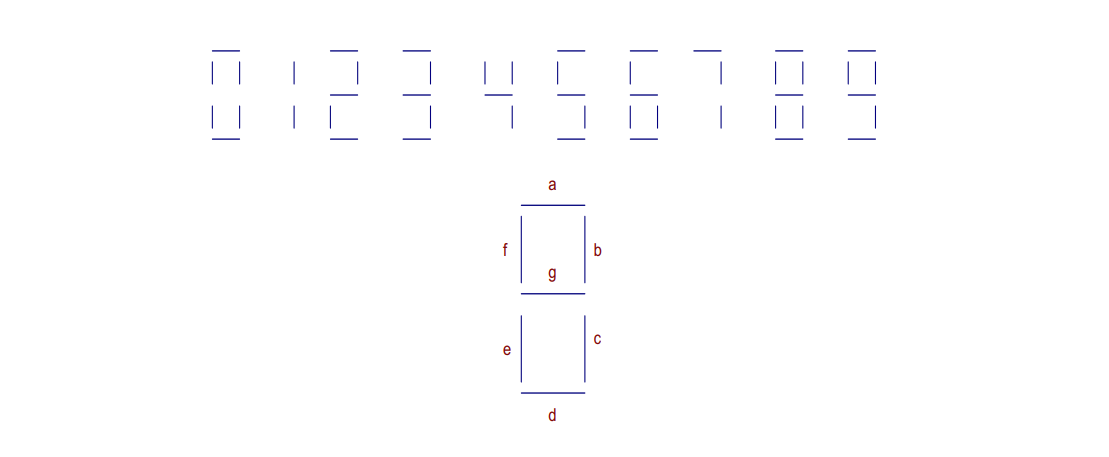
\includegraphics[width=0.4\linewidth]{7seg.png}
\end{figure}

\textit{Si vuole pilotare un singolo segmento di un display a 7 segmenti a partire dalla cifra BCD in ingresso $a,b,c,d$.}

\medskip
\noindent Si costruisce la tabella di verità del segmento (con $a\leftrightarrow$ bit più significativo, $d\leftrightarrow$ bit meno significativo) e si segnano come \textbf{don't care} ($\times$) le combinazioni che non corrispondono a nessuna cifra BCD (cioè da 10 a 15), in modo da poter scegliere il loro valore così da semplificare il circuito:

\begin{center}
\begin{tabular}{cccc|c}
\toprule
$a$&$b$&$c$&$d$ & uscita\\
\midrule
0&0&0&0 & 0\\
0&0&0&1 & 1\\
0&0&1&0 & 0\\
0&0&1&1 & 0\\
0&1&0&0 & 1\\
0&1&0&1 & 0\\
0&1&1&0 & 0\\
0&1&1&1 & 1\\
1&0&0&0 & 0\\
1&0&0&1 & 0\\
\multicolumn{4}{c|}{1010 -- 1111} & $\times\;\times\;\times\;\times\;\times\;\times$\\
\bottomrule
\end{tabular}
\end{center}

\noindent La 2\textsuperscript{a} forma canonica (POS) del segmento, prima della semplificazione, è:
\[
F(a,b,c,d)=(a+b+c+d)\cdot(a+b+c+\overline{d})\cdot(a+\overline{b}+\overline{c}+\overline{d})
\]

\noindent Riportando la funzione (con i don't care) sulla mappa di Karnaugh a 4 variabili $cd\backslash ab$ e scegliendo opportunamente il valore dei don't care, si semplifica notevolmente il circuito:

\begin{center}
\begin{tikzpicture}[scale=0.78]
\draw (0,0) grid (4,4);
\node[font=\small] at (0.5,4.35) {00};
\node[font=\small] at (1.5,4.35) {01};
\node[font=\small] at (2.5,4.35) {11};
\node[font=\small] at (3.5,4.35) {10};
\node[font=\small, anchor=east] at (-0.1,3.5) {00};
\node[font=\small, anchor=east] at (-0.1,2.5) {01};
\node[font=\small, anchor=east] at (-0.1,1.5) {11};
\node[font=\small, anchor=east] at (-0.1,0.5) {10};
\node[font=\small] at (-0.7,4.35) {$cd{\backslash}ab$};
\node at (0.5,3.5) {0}; \node at (1.5,3.5) {1}; \node at (2.5,3.5) {$\times$}; \node at (3.5,3.5) {0};
\node at (0.5,2.5) {1}; \node at (1.5,2.5) {0}; \node at (2.5,2.5) {$\times$}; \node at (3.5,2.5) {$\times$};
\node at (0.5,1.5) {0}; \node at (1.5,1.5) {1}; \node at (2.5,1.5) {$\times$}; \node at (3.5,1.5) {$\times$};
\node at (0.5,0.5) {0}; \node at (1.5,0.5) {0}; \node at (2.5,0.5) {$\times$}; \node at (3.5,0.5) {$\times$};
\end{tikzpicture}
\end{center}

\noindent Scegliendo i don't care in modo da formare i raggruppamenti più grandi possibile, l'espressione semplificata diventa:
\[
a+c\overline{d}+\overline{b}c+b\overline{c} = a+c\overline{d}+(b\oplus c)
\]
molto più corta e immediata da realizzare rispetto alla forma canonica di partenza.

\defbox{I \textbf{don't care} si scelgono in modo da semplificare il più possibile il circuito risultante.}

% ======================================================================
% circuito half adder — ingressi correttamente biforcati
\section{Sommatori}

\subsection{Semi-sommatore (half adder)}

\noindent Un \textbf{semi-sommatore} (half adder) è un circuito combinatorio in grado di eseguire la somma di due singoli bit ($a_i$ e $b_i$). Esso produce due uscite: il bit di somma $\Sigma_i$ e il bit di riporto generato $C_{i+1}$ (carry out). L'equazione logica che descrive la somma è un'operazione XOR ($\Sigma_i = a_i \oplus b_i$), mentre il riporto è dato da un'operazione AND ($C_{i+1} = a_i \cdot b_i$). 
Il limite del semi-sommatore è che non prevede un ingresso per il riporto proveniente da uno stadio precedente, limitandone l'utilizzo al solo bit meno significativo di un'addizione su più bit.

\begin{center}
\begin{circuitikz}[scale=1.0, every node/.style={scale=1.0}]
% Porte
\node[xor port] (XH) at (0, 1.5) {};
\node[and port] (AH) at (0, 0) {};

% Nodi di ingresso (allineati dinamicamente alle porte per evitare linee storte)
\coordinate (Ain) at (-2.5, 0 |- XH.in 1);
\coordinate (Bin) at (-2.5, 0 |- XH.in 2);
\node[left] at (Ain) {$a_i$};
\node[left] at (Bin) {$b_i$};

% Connessioni principali
\draw (Ain) -- (XH.in 1);
\draw (Bin) -- (XH.in 2);

% Derivazioni (i pallini sono centrati dinamicamente sulla linea)
\coordinate (Atap) at (-1.8, 0 |- XH.in 1);
\coordinate (Btap) at (-1.1, 0 |- XH.in 2);

\draw (Atap) to[short, *-] (Atap |- AH.in 1) -- (AH.in 1);
\draw (Btap) to[short, *-] (Btap |- AH.in 2) -- (AH.in 2);

% Uscite
\draw (XH.out) -- ++(0.7,0) node[right]{$\Sigma_i$};
\draw (AH.out) -- ++(0.7,0) node[right]{$C_{i+1}$};

\end{circuitikz}
\end{center}

\noindent Tabella di verità del semi-sommatore:

\begin{center}
\begin{tabular}{cc|cc}
\toprule
$a_i$ & $b_i$ & $\Sigma_i$ & $C_{i+1}$\\
\midrule
0&0&0&0\\
0&1&1&0\\
1&0&1&0\\
1&1&0&1\\
\bottomrule
\end{tabular}
\end{center}

\subsection{Sommatore completo (full adder)}

\noindent Il \textbf{sommatore completo} (full adder) risolve il limite del semi-sommatore aggiungendo un terzo ingresso $C_i$ per il riporto proveniente da uno stadio precedente. L'uscita somma $\Sigma_i$ vale 1 se il numero di ingressi a 1 è dispari, mentre il riporto $C_{i+1}$ vale 1 se almeno due ingressi sono a 1.
\medskip

\noindent Il circuito può essere ottenuto combinando due semi-sommatori e una porta OR finale per i riporti, in modo da tenere conto di tutti gli addendi:

\begin{center}
\begin{circuitikz}[scale=1.0, every node/.style={scale=1.0}]
% Primo HA
\draw (0, 0.3) rectangle (2.5, 2.3);
\node at (1.25, 1.3) {HA 1};
\node[right] at (0, 1.8) {$a_i$};
\node[right] at (0, 0.8) {$b_i$};
\node[left] at (2.5, 1.8) {$\Sigma'_i$};
\node[left] at (2.5, 0.8) {$C'_i$};

% Secondo HA
\draw (4.5, 1.3) rectangle (7.0, 3.3);
\node at (5.75, 2.3) {HA 2};
\node[right] at (4.5, 2.8) {$C_i$};
\node[right] at (4.5, 1.8) {$\Sigma'_i$};
\node[left] at (7.0, 2.8) {$\Sigma_i$};
\node[left] at (7.0, 1.8) {$C''_i$};

% OR gate
\node[or port] (OR) at (9.5, 1.3) {};

% Connessioni primo HA
\draw (-1.5, 1.8) node[left] {$a_i$} -- (0, 1.8);
\draw (-1.5, 0.8) node[left] {$b_i$} -- (0, 0.8);

% Connessioni intermedie e Cin
\draw (2.5, 1.8) -- (4.5, 1.8); % Linea dritta, nessun gradino!
\draw (-1.5, 2.8) node[left] {$C_i$} -- (4.5, 2.8); % Linea dritta, nessun gradino!

% Connessioni Carry
\draw (2.5, 0.8) -- (8.2, 0.8) |- (OR.in 2);
\draw (7.0, 1.8) -- (8.2, 1.8) |- (OR.in 1);

% Uscite finali
\draw (7.0, 2.8) -- (10.5, 2.8) node[right] {$\Sigma_i$};
\draw (OR.out) -- (10.5, 1.3) node[right] {$C_{i+1}$};

\end{circuitikz}
\end{center}

\noindent Tabella di verità del sommatore completo (con $\Sigma_i'$, $C_{i+1}'$ uscite del primo HA):

\begin{center}
\begin{tabular}{ccc|ccc}
\toprule
$a_i$ & $b_i$ & $C_i$ & $\Sigma_i'$ & $\Sigma_i$ & $C_{i+1}$\\
\midrule
0&0&0&0&0&0\\
0&0&1&0&1&0\\
0&1&0&1&1&0\\
0&1&1&1&0&1\\
1&0&0&1&1&0\\
1&0&1&1&0&1\\
1&1&0&0&0&1\\
1&1&1&0&1&1\\
\bottomrule
\end{tabular}
\end{center}

\subsubsection*{Logica dietro la tabella di verità}

Le due uscite del full adder obbediscono a regole semplici che si ricavano direttamente dal significato fisico della somma binaria.

\begin{itemize}
    \item \textbf{Bit di somma $\Sigma_i$ — ``parità'' degli ingressi:}
    $\Sigma_i = 1$ ogni volta che il numero totale di ingressi a \textbf{1} è \emph{dispari} (uno solo oppure tutti e tre). Questo coincide esattamente con l'\textbf{XOR a tre vie}:
    \[
        \Sigma_i = a_i \oplus b_i \oplus C_i
    \]
    Si può verificare intuitivamente: $1+1+0 = 2_{10} = 10_2$, la cifra delle unità è \textbf{0}; $1+1+1 = 3_{10} = 11_2$, la cifra delle unità è \textbf{1}. In entrambi i casi conta solo la parità degli addendi.

    \item \textbf{Bit di riporto $C_{i+1}$ — ``maggioranza'' degli ingressi:}
    $C_{i+1} = 1$ ogni volta che \emph{almeno due} ingressi su tre sono a \textbf{1} (funzione di maggioranza). Algebricamente:
    \[
        C_{i+1} = a_i b_i + b_i C_i + a_i C_i
    \]
    Ogni termine rappresenta una coppia che, sommata, produce riporto ($1+1 \ge 2$).
\end{itemize}

Queste due formule — e quindi l'intera tabella — si ricavano senza dover enumerare tutti gli 8 casi: basta ricordare che $\Sigma_i$ conta la \emph{parità} e $C_{i+1}$ la \emph{maggioranza} dei tre bit in ingresso.

% ======================================================================
\chapter{Sommatori, complemento a 2 e codici}

\section{Esempio: sommatore a 4 bit}
\textit{(27 marzo 2026)}

Collegando in cascata 4 sommatori completi (Full Adder, FA) si ottiene un circuito per l'addizione a 4 bit, noto come \textbf{Ripple-Carry Adder} (sommatore a propagazione di riporto). Ogni stadio $i$ somma i bit $a_i$ e $b_i$ più il riporto dello stadio precedente ($C_i$), generando il bit di somma ($\Sigma_i$) e il nuovo riporto ($C_{i+1}$) per lo stadio successivo.

\begin{center}
\begin{circuitikz}[scale=0.72, every node/.style={scale=0.72}]
% 4 FA in cascata
\foreach \i/\xi in {0/0, 1/2.6, 2/5.2, 3/7.8}{
  \draw (\xi,0) rectangle (\xi+2.0, 1.8);
  \node at (\xi+1.0, 0.9) {FA};
}
% Ingressi a_i
\foreach \i/\xi/\lab in {0/0/$a_0$, 1/2.6/$a_1$, 2/5.2/$a_2$, 3/7.8/$a_3$}{
  \draw[-latex] (\xi+0.6, 2.4) -- (\xi+0.6, 1.8) node[midway,right,font=\small]{\lab};
}
% Ingressi b_i
\foreach \i/\xi/\lab in {0/0/$b_0$, 1/2.6/$b_1$, 2/5.2/$b_2$, 3/7.8/$b_3$}{
  \draw[-latex] (\xi+1.4, 2.4) -- (\xi+1.4, 1.8) node[midway,right,font=\small]{\lab};
}
% Carry chain: C0 entra da sinistra, C1..C4 si propagano
\draw[-latex] (-1.0, 0.9) -- (0, 0.9) node[midway,above,font=\small]{$C_0$};
\draw[-latex] (2.0,0.9) -- (2.6,0.9) node[midway,above,font=\small]{$C_1$};
\draw[-latex] (4.6,0.9) -- (5.2,0.9) node[midway,above,font=\small]{$C_2$};
\draw[-latex] (7.2,0.9) -- (7.8,0.9) node[midway,above,font=\small]{$C_3$};
\draw[-latex] (9.8,0.9) -- (10.5,0.9) node[right,font=\small]{$C_4$};
% Uscite Sigma
\foreach \i/\xi/\lab in {0/0/$\Sigma_0$, 1/2.6/$\Sigma_1$, 2/5.2/$\Sigma_2$, 3/7.8/$\Sigma_3$}{
  \draw[-latex] (\xi+1.0, 0) -- (\xi+1.0,-0.6) node[below,font=\small]{\lab};
}
% Freccia overflow su C4
\draw[-latex,color=teal] (10.5,0.9) -- ++(0.5,0.4) node[right,font=\small,color=teal]{\textbf{bit di overflow}};
\end{circuitikz}
\end{center}

\medskip
\textbf{Esempio rapido di calcolo:}\\
Proviamo a sommare $A = 0101_2$ ($5_{10}$) e $B = 0011_2$ ($3_{10}$), ponendo il riporto iniziale $C_0 = 0$:
\begin{itemize}
    \item \textbf{Stadio 0:} $a_0(1) + b_0(1) + C_0(0) = 2 \implies \Sigma_0 = 0$, riporto $C_1 = 1$.
    \item \textbf{Stadio 1:} $a_1(0) + b_1(1) + C_1(1) = 2 \implies \Sigma_1 = 0$, riporto $C_2 = 1$.
    \item \textbf{Stadio 2:} $a_2(1) + b_2(0) + C_2(1) = 2 \implies \Sigma_2 = 0$, riporto $C_3 = 1$.
    \item \textbf{Stadio 3:} $a_3(0) + b_3(0) + C_3(1) = 1 \implies \Sigma_3 = 1$, riporto $C_4 = 0$.
\end{itemize}
Risultato corretto: $\Sigma = 1000_2$ ($8_{10}$).

\defbox{
\textbf{Bit di overflow (}$C_4$\textbf{)}: È il bit di riporto finale in uscita dal blocco più significativo. Se stiamo eseguendo addizioni su numeri binari puri (senza segno) a 4 bit e otteniamo $C_4 = 1$, il risultato supera il valore massimo rappresentabile ($15_{10}$). In questo caso si è verificato un errore di overflow.
}

\textbf{Il problema del ritardo (Delay):}\\
Il principale limite prestazionale di questo circuito è che ogni blocco FA deve "aspettare" che il blocco precedente calcoli il suo riporto. Il segnale $C$ deve letteralmente "propagarsi" a cascata (ripple) da $C_0$ fino a $C_4$. 
\begin{itemize}
    \item Se una singola porta logica ha un tempo di ritardo $\Delta T$, ogni blocco Full Adder impiega circa $3\Delta T$ per generare il riporto.
    \item In un sommatore a $n$ bit, il tempo totale $\Delta t$ cresce in modo lineare:
    \[ \Delta t = n \cdot 3\Delta T \]
\end{itemize}

\textbf{Soluzione: i sommatori Carry Look-Ahead (CLA)}\\
Per eliminare questa latenza si utilizzano circuiti più avanzati (ad anticipo di riporto). Attraverso un'apposita rete logica parallela, questi circuiti capiscono "in anticipo" se i vari stadi andranno a \emph{generare} o \emph{propagare} un riporto. In questo modo si possono calcolare tutte le uscite simultaneamente, con un ritardo bassissimo e logaritmico (o indipendente) rispetto alla lunghezza $n$ della parola.

\section{Modularità e Design Gerarchico}

Nella progettazione digitale moderna, si sfrutta ampiamente il concetto di \textbf{modularità}.

\defbox{\textbf{Design Modulare}: un approccio in cui il sistema complesso viene suddiviso in sottomoduli standard e interscambiabili (es. usare i Full Adder base per costruire un sommatore a $n$ bit). Questi moduli possono essere aggiunti, rimossi o sostituiti senza dover alterare o riprogettare il resto del sistema.}

\noindent I vantaggi principali includono:
\begin{itemize}
    \item \textbf{Astrazione}: chi progetta un processore non deve preoccuparsi della logica a porte interne al singolo FA, ma ne considera solo gli ingressi e le uscite.
    \item \textbf{Riutilizzo e Semplificazione}: un modulo testato e verificato può essere riutilizzato in più punti, rendendo il collaudo molto più affidabile.
\end{itemize}

\section{Sottrattori e numeri negativi}
\textit{(27 marzo 2026 -- cont.)}

Nei circuiti digitali, per rappresentare anche i numeri negativi, si deve "sacrificare" un bit (di solito il più significativo) per indicare il segno. Esistono diverse tecniche per farlo:

\textbf{1. Modulo e Segno}\\
Il bit più a sinistra indica il segno ($0$ = positivo, $1$ = negativo), mentre i restanti bit indicano il valore assoluto. Questa tecnica presenta un problema pratico: lo zero ha due rappresentazioni diverse. Ad esempio su 4 bit, $0000$ ($+0$) e $1000$ ($-0$) indicano entrambi il numero zero. Questo complica inutilmente i circuiti di calcolo.

\textbf{2. La teoria dei Complementi}\\
Per risolvere questo problema si utilizza un metodo matematico chiamato \emph{complemento}. Dato un numero $N$ espresso in una certa base $r$ e lungo $n$ cifre, si definiscono due tipi di complemento:
\begin{itemize}
    \item \textbf{Complemento alla base diminuita (base $r-1$):} \\
    Si definisce come $C_{r-1}(N) = (r^n - 1) - N$. Poiché $r^n - 1$ è il numero massimo rappresentabile ($N_{\max}$), si ottiene sottraendo il numero $N$ dal valore massimo.
    \item \textbf{Complemento alla base (base $r$):} \\
    Si definisce come $C_r(N) = r^n - N$. Essendo $r^n = (r^n - 1) + 1$, equivale matematicamente ad aggiungere $1$ al complemento alla base diminuita.
\end{itemize}

\textbf{Applicazione al Sistema Binario (Base 2):}\\
Nei sistemi binari (base $r=2$), queste due definizioni prendono il nome di \textbf{Complemento a 1} e \textbf{Complemento a 2}.

\textbf{Complemento a 1 ($C_1$):}
\[ C_1(N) = (2^n - 1) - N \]
Poiché $2^n-1$ è un numero composto da tutti "1" (es. $1111_2$), sottrarre $N$ significa banalmente \emph{invertire tutti i singoli bit} di $N$ (ogni bit $N_i$ diventa $\overline{N}_i$):
\[ C_1(N) = \overline{N}_{n-1}\cdots\overline{N}_1\overline{N}_0 \]

\textbf{Complemento a 2 ($C_2$):}
\[ C_2(N) = 2^n - N \]
Come visto prima, possiamo riscriverlo come $(2^n - 1 - N) + 1$. Questo significa che per calcolare il complemento a 2 basta prendere il complemento a 1 e sommare 1:
\[ C_2(N) = C_1(N) + 1 = \overline{N}_{n-1}\cdots\overline{N}_1\overline{N}_0 + 1 \]

\noindent\textit{Proprietà fondamentale:} Applicare due volte il complemento a 2 restituisce il numero originale, ovvero $C_2(C_2(N)) = N$.

\defbox{
Il \textbf{complemento a 2} è la notazione standard per rappresentare numeri interi con segno nei calcolatori. A differenza della codifica a modulo e segno, garantisce un'unica rappresentazione per lo zero (es. $0000$) e permette di eseguire somme e sottrazioni con la stessa rete logica hardware.
}

\noindent\textbf{Regola pratica per calcolare il complemento a 2 di un numero}:
\begin{enumerate}
    \item Si parte dal numero binario positivo (es. $+3_{10} = 0011_2$).
    \item Si invertono tutti i bit (complemento a 1): $0011 \to 1100$.
    \item Si somma $1$ al risultato: $1100 + 1 = 1101$. 
\end{enumerate}
Quindi $-3_{10} = 1101_2$ in complemento a 2 su 4 bit.

\medskip
Se verifichiamo calcolando l'addizione $-3 + 3$, avremo: $1101 + 0011 = 1\,0000$. Poiché lavoriamo a 4 bit, l'uno più a sinistra (il \emph{carry out} uscente) cade fuori dalla dimensione dei registri e viene ignorato. Il risultato memorizzato è esattamente $0000$, ovvero 0.

\subsection{Circuito sommatore/sottrattore a 4 bit}

Un grande vantaggio della codifica in complemento a 2 è la possibilità di eseguire sia addizioni che sottrazioni utilizzando il \textbf{medesimo circuito hardware}. Per farlo, si estende il classico sommatore (ripple-carry adder) introducendo delle porte logiche XOR sugli ingressi del secondo operando e sfruttando il riporto iniziale $C_0$ come segnale di controllo (selettore d'operazione).

\begin{center}
\begin{circuitikz}[scale=0.9, every node/.style={scale=0.9}]
\tikzset{FA/.style={draw, minimum width=1.6cm, minimum height=1.6cm, align=center}}

% Disegno dei 4 blocchi Full Adder
\foreach \i/\x in {0/0, 1/3.5, 2/7.0, 3/10.5} {
    \node[FA] (FA\i) at (\x,0) {FA$_\i$};
}

% Linea comune per C0 (selezione operazione)
\coordinate (C0line) at (-1.5, 4.0);
\draw (-1.5, 4.0) node[left] {$C_0$ (\textsf{0}=Add, \textsf{1}=Sub)} -- (11.0, 4.0);

% Connessione C0 come riporto in ingresso del primo FA
\draw[-latex] (-1.5, 4.0) -- (-1.5, 0) -- (FA0.west) node[midway, above] {$C_0$};

\foreach \i in {0,1,2,3} {
    % a_i input
    \draw[-latex] (FA\i.120 |- 0, 4.8) node[above] {$a_\i$} -- (FA\i.120);
    
    % b_i input e XOR
    \node[xor port, rotate=-90, scale=0.7] (XOR\i) at (FA\i.60 |- 0, 2.5) {};
    \draw[-latex] (XOR\i.out) -- (FA\i.60);
    
    % Connessione di b_i all'ingresso 1 dello XOR
    \draw (XOR\i.in 1) -- (XOR\i.in 1 |- 0, 4.8) node[above] {$b_\i$};
    
    % Connessione di C0 all'ingresso 2 dello XOR
    \draw (XOR\i.in 2) -- (XOR\i.in 2 |- C0line) node[circle, fill, inner sep=1.2pt] {};
}

% Carry chain tra i FA
\draw[-latex] (FA0.east) -- (FA1.west) node[midway, above] {$C_1$};
\draw[-latex] (FA1.east) -- (FA2.west) node[midway, above] {$C_2$};
\draw[-latex] (FA2.east) -- (FA3.west) node[midway, above] {$C_3$};

% Uscita C4
\draw[-latex] (FA3.east) -- ++(1.5,0) coordinate (C4out) node[above] {$C_4$};

% Uscite Somma (Sigma)
\foreach \i in {0,1,2,3} {
    \draw[-latex] (FA\i.south) -- ++(0,-1.0) node[below] {$\Sigma_\i$};
}

% XOR finale per l'overflow (E)
\node[xor port, scale=0.8] (E_XOR) at (13.5, -2.0) {};

% Preleviamo C3
\coordinate (tapC3) at (8.75, 0);
\draw (tapC3) node[circle, fill, inner sep=1.2pt] {} |- (E_XOR.in 2);

% Preleviamo C4
\coordinate (tapC4) at (12.0, 0);
\draw (tapC4) node[circle, fill, inner sep=1.2pt] {} |- (E_XOR.in 1);

\draw[-latex] (E_XOR.out) -- ++(0.8,0) node[right] {$E_{Overf}$};

\end{circuitikz}
\end{center}

Il funzionamento del circuito dipende dal valore del segnale di controllo $C_0$:

\begin{itemize}[leftmargin=1.5em]
    \item \textbf{Se $C_0=0$ (Addizione)}: la porta XOR riceve uno 0 e si comporta come un buffer trasparente ($b_i \oplus 0 = b_i$). Inoltre, il riporto in ingresso al primo FA è anch'esso 0. Il circuito esegue quindi una normale addizione: $S = a + b$.
    
    \item \textbf{Se $C_0=1$ (Sottrazione)}: la porta XOR riceve un 1 e si comporta come un invertitore logico ($b_i \oplus 1 = \overline{b}_i$), calcolando il complemento a 1 di $b$. Il riporto in ingresso al primo FA fornisce un ulteriore $+1$. In questo modo, il circuito calcola internamente l'espressione $a + \overline{b} + 1$. Poiché $\overline{b} + 1$ equivale a $-b$ (in complemento a 2), l'operazione totale svolta è esattamente la sottrazione: $S = a - b$.
    
    \item \textbf{Errore di Overflow ($E$)}: lavorando con un numero fisso di bit (in questo caso 4 bit, intervallo rappresentabile da $-8$ a $+7$), può accadere che il risultato reale dell'operazione sia al di fuori di questo intervallo. Questo errore prende il nome di \emph{overflow} e viene segnalato tramite una porta XOR applicata agli ultimi due riporti generati ($E = C_3 \oplus C_4$). Se $E=1$, si ha un \emph{overflow} e il risultato non è valido.
\end{itemize}

In generale, lavorando in complemento a 2 con 4 bit, si rappresenta l'intervallo da $-8$ a $+7$:
\begin{itemize}[leftmargin=1.5em]
    \item[\small$\blacksquare$] Se $\Sigma_3 = 0 \;\Leftrightarrow\;$ il risultato $\Sigma$ è positivo o nullo.
    \item[\small$\blacksquare$] Se $\Sigma_3 = 1 \;\Leftrightarrow\;$ il risultato $\Sigma$ è negativo.
\end{itemize}

\begin{center}
\begin{tikzpicture}[scale=1.1]
% Cerchio complemento a 2 a 4 bit
\draw (0,0) circle (2.0cm);
\foreach \angle/\val/\bin in {
  90/0/0000, 67.5/1/0001, 45/2/0010, 22.5/3/0011,
  0/4/0100, -22.5/5/0101, -45/6/0110, -67.5/7/0111,
  -90/-8/1000, -112.5/-7/1001, -135/-6/1010, -157.5/-5/1011,
  180/-4/1100, 157.5/-3/1101, 135/-2/1110, 112.5/-1/1111
}{
  \node[font=\tiny] at ({2.4*cos(\angle)},{2.4*sin(\angle)}) {\val};
  \node[font=\tiny] at ({1.6*cos(\angle)},{1.6*sin(\angle)}) {\bin};
}
\node[font=\small\bfseries, align=center] at (0,0) {4-bit};
% assi cardinali
\foreach \a in {0,90,180,270}{
  \draw[gray,thin] ({1.9*cos(\a)},{1.9*sin(\a)}) -- ({2.1*cos(\a)},{2.1*sin(\a)});
}
\end{tikzpicture}
\end{center}

% ======================================================================
\chapter{Codice Gray e ASCII}
\textit{(30 marzo 2026)}

\section{Codice Gray}

\defbox{
Il \textbf{Codice Gray} è una codifica binaria non pesata in cui due valori consecutivi differiscono sempre e solo per \emph{un singolo bit}.
}

\noindent I vantaggi principali del codice Gray rispetto al normale codice binario puro sono:
\begin{itemize}[leftmargin=1.5em]
    \item \textbf{Prevenzione dei glitch (stati spuri)}: in un contatore binario normale, il passaggio ad esempio da $3$ ($011_2$) a $4$ ($100_2$) comporta la commutazione simultanea di 3 bit. Fisicamente, i bit non commuteranno mai nel medesimo istante esatto, causando passaggi in stati intermedi transitori errati (es. $011 \to 111 \to 100$). Con il codice Gray, cambiando un solo bit per ogni incremento, le transizioni sono sempre sicure e prive di glitch.
    \item \textbf{Riduzione della dissipazione di potenza}: in tecnologie CMOS, la potenza dinamica è dissipata principalmente durante le commutazioni di stato logico. Poiché nel codice Gray commuta sempre e solo un bit alla volta, la potenza dissipata è minima e costante nel tempo, rendendolo ideale per contatori a basso consumo o per le macchine a stati finiti.
\end{itemize}

\begin{minipage}[t]{0.30\linewidth}
\vspace{0pt}
\centering
\begin{tabular}{r c c}
\toprule
Dec. & Binario & Gray\\
\midrule
$0$  & $0000$ & $0000$ \\
$1$  & $0001$ & $0001$ \\
$2$  & $0010$ & $0011$ \\
$3$  & $0011$ & $0010$ \\
$4$  & $0100$ & $0110$ \\
$5$  & $0101$ & $0111$ \\
$6$  & $0110$ & $0101$ \\
$7$  & $0111$ & $0100$ \\
\midrule
$8$  & $1000$ & $1100$ \\
$9$  & $1001$ & $1101$ \\
$10$ & $1010$ & $1111$ \\
$11$ & $1011$ & $1110$ \\
$12$ & $1100$ & $1010$ \\
$13$ & $1101$ & $1011$ \\
$14$ & $1110$ & $1001$ \\
$15$ & $1111$ & $1000$ \\
\bottomrule
\end{tabular}
\end{minipage}%
\hfill
\begin{minipage}[t]{0.66\linewidth}
\vspace{0pt}
\noindent Dato un numero a $n$ bit (dove l'indice $n-1$ rappresenta il bit più significativo, MSB):

\medskip
\textbf{Conversione Binario $\to$ Gray}:\\
Il bit più significativo resta invariato. Ogni altro bit Gray si calcola come XOR tra il bit binario nella stessa posizione e il bit binario precedente (più significativo).
\[
G_{n-1} = B_{n-1} \qquad G_k = B_k \oplus B_{k+1} \quad \text{per } k < n-1
\]

\medskip
\textbf{Conversione Gray $\to$ Binario}:\\
Il bit più significativo resta invariato. Ogni altro bit binario si ottiene come XOR tra il bit Gray nella stessa posizione e il \emph{bit binario appena calcolato} nella posizione più significativa adiacente.
\[
B_{n-1} = G_{n-1} \qquad B_k = G_k \oplus B_{k+1} \quad \text{per } k < n-1
\]
\textit{(Nota matematica: sviluppando la ricorsione si nota che equivale alla formula $B_k = G_k \oplus G_{k+1} \oplus \dots \oplus G_{n-1}$, spesso implementata in hardware per velocizzare i tempi di calcolo parallelo).}
\end{minipage}

\subsection{Circuiti di conversione}

\begin{fitcenter}
\begin{circuitikz}[scale=0.85, every node/.style={scale=0.85}]

% ============================================================
% CIRCUITO BG  (Binario -> Gray)  —  colonna sinistra
% ============================================================
% G_{n-1} = B_{n-1} (passthrough), G_k = B_k XOR B_{k+1}

% Porte XOR per G0, G1, G2
\node[xor port] (BG0) at (2.0, 5.0) {};   % G0 = B0 XOR B1
\node[xor port] (BG1) at (2.0, 3.5) {};   % G1 = B1 XOR B2
\node[xor port] (BG2) at (2.0, 2.0) {};   % G2 = B2 XOR B3

% --- Ingresso B0 ---
\draw (-1.0, 0 |- BG0.in 1) node[left]{$B_0$} -- (BG0.in 1);

% --- Ingresso B1 ---
\draw (-1.0, 4.25) node[left]{$B_1$} -- (0.0, 4.25);
\node[circle, fill, inner sep=1.5pt] at (0.0, 4.25) {};
\draw (0.0, 4.25) |- (BG0.in 2);
\draw (0.0, 4.25) |- (BG1.in 1);

% --- Ingresso B2 ---
\draw (-1.0, 2.75) node[left]{$B_2$} -- (0.2, 2.75);
\node[circle, fill, inner sep=1.5pt] at (0.2, 2.75) {};
\draw (0.2, 2.75) |- (BG1.in 2);
\draw (0.2, 2.75) |- (BG2.in 1);

% --- Ingresso B3 ---
\draw (-1.0, 1.0) node[left]{$B_3$} -- (4.3, 1.0) node[right]{$G_3$};
\node[circle, fill, inner sep=1.5pt] at (0.4, 1.0) {};
\draw (0.4, 1.0) |- (BG2.in 2);

% --- Uscite Gray ---
\draw (BG0.out) -- (4.3, 0 |- BG0.out) node[right]{$G_0$};
\draw (BG1.out) -- (4.3, 0 |- BG1.out) node[right]{$G_1$};
\draw (BG2.out) -- (4.3, 0 |- BG2.out) node[right]{$G_2$};

\node[below, font=\small\bfseries, color=teal] at (2.0, 0.4) {Conversione B$\to$G};

% ============================================================
% CIRCUITO GB  (Gray -> Binario)  —  colonna destra
% ============================================================
% B_{n-1} = G_{n-1}, poi B_k = G_k XOR B_{k+1}

% Porte XOR per B0, B1, B2
\node[xor port] (GB0) at (9.5, 5.0) {};   % B0 = G0 XOR B1
\node[xor port] (GB1) at (9.5, 3.5) {};   % B1 = G1 XOR B2
\node[xor port] (GB2) at (9.5, 2.0) {};   % B2 = G2 XOR B3

% --- Ingresso G0 ---
\draw (6.5, 0 |- GB0.in 1) node[left]{$G_0$} -- (GB0.in 1);

% --- Ingresso G1 ---
\draw (6.5, 0 |- GB1.in 1) node[left]{$G_1$} -- (GB1.in 1);

% --- Ingresso G2 ---
\draw (6.5, 0 |- GB2.in 1) node[left]{$G_2$} -- (GB2.in 1);

% --- Ingresso G3 e Uscita B3 (passthrough) ---
\draw (6.5, 1.0) node[left]{$G_3$} -- (11.8, 1.0) node[right]{$B_3$};

% --- Uscita B0 ---
\draw (GB0.out) -- (11.8, 0 |- GB0.out) node[right]{$B_0$};

% --- Uscita B1 e feedback ---
\draw (GB1.out) -- (11.8, 0 |- GB1.out) node[right]{$B_1$};
\node[circle, fill, inner sep=1.5pt] at (10.5, 0 |- GB1.out) {};
\draw (10.5, 0 |- GB1.out) -- (10.5, 4.25) -- (7.5, 4.25) |- (GB0.in 2);

% --- Uscita B2 e feedback ---
\draw (GB2.out) -- (11.8, 0 |- GB2.out) node[right]{$B_2$};
\node[circle, fill, inner sep=1.5pt] at (10.7, 0 |- GB2.out) {};
\draw (10.7, 0 |- GB2.out) -- (10.7, 2.75) -- (7.7, 2.75) |- (GB1.in 2);

% --- Feedback da B3 ---
\node[circle, fill, inner sep=1.5pt] at (10.9, 1.0) {};
\draw (10.9, 1.0) -- (10.9, 1.35) -- (7.9, 1.35) |- (GB2.in 2);

\node[below, font=\small\bfseries, color=teal] at (9.5, 0.4) {Conversione G$\to$B};

\end{circuitikz}
\end{fitcenter}

% ======================================================================
\subsection{Esercizi svolti: conversioni passo-passo}

Applichiamo le formule ai due casi classici usando numeri a \textbf{4 bit}
($B_3 B_2 B_1 B_0$, con $B_3$ = MSB).

% ------------------------------------------------------------------
\subsubsection*{Esercizio 1 — Binario $\to$ Gray: \quad $1011_2 \;(=11_{10})$}

La regola è: $G_3 = B_3$, poi $G_k = B_k \oplus B_{k+1}$.

\medskip
\begin{center}
\begin{tabular}{c|c|c|l}
\toprule
Bit & Formula & Calcolo & Risultato\\
\midrule
$G_3$ & $B_3$ & $1$ & $G_3 = \mathbf{1}$ \\
$G_2$ & $B_2 \oplus B_3$ & $0 \oplus 1$ & $G_2 = \mathbf{1}$ \\
$G_1$ & $B_1 \oplus B_2$ & $1 \oplus 0$ & $G_1 = \mathbf{1}$ \\
$G_0$ & $B_0 \oplus B_1$ & $1 \oplus 1$ & $G_0 = \mathbf{0}$ \\
\bottomrule
\end{tabular}
\end{center}

\medskip
\noindent Si parte dal MSB e si scende verso il LSB, applicando uno XOR bit a bit con il vicino più significativo già noto:

\[
\underbrace{1}_{B_3}\;\underbrace{0}_{B_2}\;\underbrace{1}_{B_1}\;\underbrace{1}_{B_0}
\;\xrightarrow{\text{B}\to\text{G}}\;
\underbrace{1}_{G_3}\;\underbrace{1}_{G_2}\;\underbrace{1}_{G_1}\;\underbrace{0}_{G_0}
\quad\Rightarrow\quad \boxed{1110_G}
\]

\vspace{1.5em}

% ------------------------------------------------------------------
\subsubsection*{Esercizio 2 — Gray $\to$ Binario: \quad $1110_G$}

La regola è: $B_3 = G_3$, poi $B_k = G_k \oplus B_{k+1}$ (si usa il binario \emph{già calcolato} al passo precedente, non il Gray).

\medskip
\begin{center}
\begin{tabular}{c|c|c|l}
\toprule
Bit & Formula & Calcolo & Risultato\\
\midrule
$B_3$ & $G_3$ & $1$ & $B_3 = \mathbf{1}$ \\
$B_2$ & $G_2 \oplus B_3$ & $1 \oplus 1$ & $B_2 = \mathbf{0}$ \\
$B_1$ & $G_1 \oplus B_2$ & $1 \oplus 0$ & $B_1 = \mathbf{1}$ \\
$B_0$ & $G_0 \oplus B_1$ & $0 \oplus 1$ & $B_0 = \mathbf{1}$ \\
\bottomrule
\end{tabular}
\end{center}

\medskip
\noindent Anche qui si procede dall'MSB verso l'LSB, ma ogni XOR usa il \emph{bit binario appena ricavato} (non il Gray):

\[
\underbrace{1}_{G_3}\;\underbrace{1}_{G_2}\;\underbrace{1}_{G_1}\;\underbrace{0}_{G_0}
\;\xrightarrow{\text{G}\to\text{B}}\;
\underbrace{1}_{B_3}\;\underbrace{0}_{B_2}\;\underbrace{1}_{B_1}\;\underbrace{1}_{B_0}
\quad\Rightarrow\quad \boxed{1011_2 = 11_{10}}
\]

\vspace{0.5em}
\noindent\textit{I due esercizi si invertono a vicenda: il risultato di Esercizio~2 coincide esattamente con il punto di partenza di Esercizio~1, confermando la correttezza delle due conversioni.}

\vspace{1.5em}

% ------------------------------------------------------------------
\subsubsection*{Esercizio 3 — Binario $\to$ Gray: \quad $1101_2 \;(=13_{10})$}

\medskip
\begin{center}
\begin{tabular}{c|c|c|l}
\toprule
Bit & Formula & Calcolo & Risultato\\
\midrule
$G_3$ & $B_3$ & $1$ & $G_3 = \mathbf{1}$ \\
$G_2$ & $B_2 \oplus B_3$ & $1 \oplus 1$ & $G_2 = \mathbf{0}$ \\
$G_1$ & $B_1 \oplus B_2$ & $0 \oplus 1$ & $G_1 = \mathbf{1}$ \\
$G_0$ & $B_0 \oplus B_1$ & $1 \oplus 0$ & $G_0 = \mathbf{1}$ \\
\bottomrule
\end{tabular}
\end{center}

\[
1101_2 \;\xrightarrow{\text{B}\to\text{G}}\; \boxed{1011_G}
\]

\subsubsection*{Esercizio 4 — Gray $\to$ Binario: \quad $1011_G$}

\medskip
\begin{center}
\begin{tabular}{c|c|c|l}
\toprule
Bit & Formula & Calcolo & Risultato\\
\midrule
$B_3$ & $G_3$ & $1$ & $B_3 = \mathbf{1}$ \\
$B_2$ & $G_2 \oplus B_3$ & $0 \oplus 1$ & $B_2 = \mathbf{1}$ \\
$B_1$ & $G_1 \oplus B_2$ & $1 \oplus 1$ & $B_1 = \mathbf{0}$ \\
$B_0$ & $G_0 \oplus B_1$ & $1 \oplus 0$ & $B_0 = \mathbf{1}$ \\
\bottomrule
\end{tabular}
\end{center}

\[
1011_G \;\xrightarrow{\text{G}\to\text{B}}\; \boxed{1101_2 = 13_{10}}
\]

\vspace{0.5em}
\noindent\textit{Anche qui la coppia Esercizio~3 e Esercizio~4 è inversa, come atteso.}


% ======================================================================
\section{Codice ASCII}
 
\defbox{
L'\textbf{ASCII} (\emph{American Standard Code for Information Interchange}) è il sistema di codifica standard utilizzato storicamente per rappresentare caratteri alfanumerici e simboli di controllo nei dispositivi digitali e di telecomunicazione.
}
 
La tabella ASCII standard originale utilizza \textbf{7 bit} per codificare 128 simboli diversi ($2^7 = 128$). I codici sono suddivisi logicamente in:
\begin{itemize}[leftmargin=1.5em]
    \item \textbf{0--31 e 127}: \emph{Caratteri di controllo} (non stampabili), usati originariamente per gestire la formattazione hardware delle telescriventi (es. ritorno a capo \texttt{CR}, avanzamento riga \texttt{LF}, tabulazione \texttt{HT}) o il protocollo di comunicazione.
    \item \textbf{32--47, 58--64, 91--96, 123--126}: \emph{Simboli grafici e punteggiatura} (lo spazio è il primo carattere stampabile, codice decimale 32).
    \item \textbf{48--57}: \emph{Cifre numeriche} (da '0' a '9').
    \item \textbf{65--90}: \emph{Lettere maiuscole} (da 'A' a 'Z').
    \item \textbf{97--122}: \emph{Lettere minuscole} (da 'a' a 'z').
\end{itemize}

\noindent \textbf{Proprietà notevole}: le lettere maiuscole e le rispettive minuscole differiscono sempre esattamente per \emph{un solo bit} (il sesto bit partendo da zero, che vale $2^5=32$). 
Ad esempio, la 'A' vale $65_{10}$ ($010\textbf{0}0001_2$) e la 'a' vale $97_{10}$ ($011\textbf{0}0001_2$). Questa ingegnosa scelta progettuale non è casuale: permette ai sistemi digitali e ai microprocessori di convertire istantaneamente e a basso costo computazionale i caratteri dal maiuscolo al minuscolo semplicemente invertendo un bit (ad esempio applicando una maschera logica di tipo XOR o OR).

\medskip
 
\begin{fitcenter}
{\footnotesize\setlength{\tabcolsep}{3pt}%
\begin{tabular}{@{}c|c|c|c@{\hspace{6pt}}c|c|c|c@{\hspace{6pt}}c|c|c|c@{\hspace{6pt}}c|c|c|c@{}}
\textbf{Dec} & \textbf{Oct} & \textbf{Hex} & \textbf{Char} & \textbf{Dec} & \textbf{Oct} & \textbf{Hex} & \textbf{Char} & \textbf{Dec} & \textbf{Oct} & \textbf{Hex} & \textbf{Char} & \textbf{Dec} & \textbf{Oct} & \textbf{Hex} & \textbf{Char}\\
\hline
0&000&00&NUL & 32&040&20&(sp) & 64&100&40&@ & 96&140&60&\textasciigrave\\
1&001&01&SOH & 33&041&21&! & 65&101&41&A & 97&141&61&a\\
2&002&02&STX & 34&042&22&\textquotedbl & 66&102&42&B & 98&142&62&b\\
3&003&03&ETX & 35&043&23&\# & 67&103&43&C & 99&143&63&c\\
4&004&04&EOT & 36&044&24&\$ & 68&104&44&D & 100&144&64&d\\
5&005&05&ENQ & 37&045&25&\% & 69&105&45&E & 101&145&65&e\\
6&006&06&ACK & 38&046&26&\& & 70&106&46&F & 102&146&66&f\\
7&007&07&BEL & 39&047&27&\textquotesingle & 71&107&47&G & 103&147&67&g\\
8&010&08&BS & 40&050&28&( & 72&110&48&H & 104&150&68&h\\
9&011&09&HT & 41&051&29&) & 73&111&49&I & 105&151&69&i\\
10&012&0A&LF & 42&052&2A&* & 74&112&4A&J & 106&152&6A&j\\
11&013&0B&VT & 43&053&2B&+ & 75&113&4B&K & 107&153&6B&k\\
12&014&0C&FF & 44&054&2C&, & 76&114&4C&L & 108&154&6C&l\\
13&015&0D&CR & 45&055&2D&- & 77&115&4D&M & 109&155&6D&m\\
14&016&0E&SO & 46&056&2E&. & 78&116&4E&N & 110&156&6E&n\\
15&017&0F&SI & 47&057&2F&/ & 79&117&4F&O & 111&157&6F&o\\
16&020&10&DLE & 48&060&30&0 & 80&120&50&P & 112&160&70&p\\
17&021&11&DC1 & 49&061&31&1 & 81&121&51&Q & 113&161&71&q\\
18&022&12&DC2 & 50&062&32&2 & 82&122&52&R & 114&162&72&r\\
19&023&13&DC3 & 51&063&33&3 & 83&123&53&S & 115&163&73&s\\
20&024&14&DC4 & 52&064&34&4 & 84&124&54&T & 116&164&74&t\\
21&025&15&NAK & 53&065&35&5 & 85&125&55&U & 117&165&75&u\\
22&026&16&SYN & 54&066&36&6 & 86&126&56&V & 118&166&76&v\\
23&027&17&ETB & 55&067&37&7 & 87&127&57&W & 119&167&77&w\\
24&030&18&CAN & 56&070&38&8 & 88&130&58&X & 120&170&78&x\\
25&031&19&EM & 57&071&39&9 & 89&131&59&Y & 121&171&79&y\\
26&032&1A&SUB & 58&072&3A&: & 90&132&5A&Z & 122&172&7A&z\\
27&033&1B&ESC & 59&073&3B&; & 91&133&5B&[ & 123&173&7B&\{\\
28&034&1C&FS & 60&074&3C&\textless & 92&134&5C&\textbackslash & 124&174&7C&\textbar\\
29&035&1D&GS & 61&075&3D&= & 93&135&5D&] & 125&175&7D&\}\\
30&036&1E&RS & 62&076&3E&\textgreater & 94&136&5E&\textasciicircum & 126&176&7E&\textasciitilde\\
31&037&1F&US & 63&077&3F&? & 95&137&5F&\_ & 127&177&7F&DEL\\
\hline
\end{tabular}%
}
\end{fitcenter}
 
\begin{sloppypar}
\noindent\textit{Legenda}: le colonne da sinistra a destra mostrano decimale, ottale, esadecimale e il carattere corrispondente. I caratteri di controllo (0--31 e 127) sono abbreviati (es.\ NUL=null, SOH=start of heading, CR=carriage return, DEL=delete, ecc.).
\end{sloppypar}
 
\defbox{
\noindent\textbf{Intervalli notevoli}:
\begin{itemize}[leftmargin=1.3em]
    \item Caratteri di controllo: 0--31 e 127;
    \item Spazio: 32;
    \item Caratteri stampabili: 33--126;
    \item Cifre: 48--57 (0--9);
    \item Lettere maiuscole: 65--90 (A--Z);
    \item Lettere minuscole: 97--122 (a--z).
\end{itemize}
}

% ======================================================================
\chapter{Logica sequenziale}

\section{Circuiti combinatori e circuiti sequenziali}

Finora abbiamo visto circuiti in cui l'output dipende esclusivamente dagli input: \textbf{circuiti combinatori}.

\medskip
\noindent Esistono anche circuiti in cui lo stato delle uscite dipende anche dallo stato in cui il circuito era in precedenza: questi circuiti seguono una \textbf{logica sequenziale}.

\medskip
\noindent Nei circuiti sequenziali è necessario che ci sia una \textbf{memoria}, un feedback.

\begin{center}
\begin{circuitikz}[scale=0.85, every node/.style={scale=0.85}]
% --- Circuito combinatorio ---
\draw (0,0) rectangle (2.2,2.0);
\node at (1.1,1.0) {CC};
\foreach \y in {1.6,1.0,0.4}{
  \draw[-latex] (-1.0,\y) -- (0,\y);
}
\node[left] at (-1.0,1.0) {$I_i$};
\foreach \y in {1.6,1.0,0.4}{
  \draw[-latex] (2.2,\y) -- (3.2,\y);
}
\node[right] at (3.2,1.0) {$O_i$};
\node[below, font=\small, color=teal] at (1.1,-0.5) {logica combinatoria};
\node[below] at (1.1,-1.0) {$O_i(t)=f\big(I_i(t)\big)$};

% --- Circuito sequenziale ---
\begin{scope}[xshift=7cm]
\draw (0,0) rectangle (2.2,2.0);
\node at (1.1,1.0) {CS};
\foreach \y in {1.6,1.0,0.4}{
  \draw[-latex] (-1.0,\y) -- (0,\y);
}
\node[left] at (-1.0,1.0) {$I_i$};
\foreach \y in {1.6,1.0,0.4}{
  \draw[-latex] (2.2,\y) -- (3.2,\y);
}
\node[right] at (3.2,1.0) {$O_i$};
% feedback loop
\draw (3.0,1.6) -- (3.6,1.6) -- (3.6,-0.6) -- (-0.6,-0.6) -- (-0.6,0.4) -- (0,0.4);
\node[right, font=\scriptsize] at (3.65,1.6) {tratti di feedback};
\node[below, font=\small, color=teal] at (1.1,-1.0) {logica sequenziale};
\node[below] at (1.1,-1.5) {$O_i(t+\Delta t)=f\big(I_i(t),O_i(t)\big)$};
\end{scope}
\end{circuitikz}
\end{center}

\section{Bistabilità e oscillazione}

Il \textbf{circuito bistabile} rappresenta la forma più semplice di \textbf{memoria} in elettronica digitale. Si ottiene collegando in anello chiuso un numero \textbf{pari} di porte logiche invertenti (ad esempio porte NOT). Poiché ogni segnale viene invertito due volte, il valore che ritorna all'ingresso è uguale a quello di partenza. Questo crea un \textbf{feedback positivo} che rinforza e mantiene stabile all'infinito lo stato logico assunto all'accensione, conservando così un bit di informazione ($0$ o $1$).

\defbox{
Il problema di un semplice anello di porte NOT è che è un sistema isolato: \textbf{non è possibile modificarne lo stato} dall'esterno. Per potervi "scrivere" un nuovo bit (impostarlo a 1 o azzerarlo a 0), le porte NOT vengono sostituite con porte \textbf{NOR} o \textbf{NAND}, le quali offrono dei terminali di ingresso aggiuntivi per i segnali di controllo.
}

Se invece colleghiamo in anello chiuso un numero \textbf{dispari} di porte NOT, otteniamo un \textbf{circuito oscillante} (o \emph{ring oscillator}). L'inversione dispari fa sì che il segnale ritorni all'ingresso invertito rispetto alla partenza. Questo genera una perenne instabilità: l'uscita continua a commutare ciclicamente tra $0$ e $1$, con un periodo $T$ proporzionale al numero di porte e al ritardo di propagazione di ciascuna di esse.

\begin{center}
\begin{circuitikz}[scale=0.9, every node/.style={scale=0.9}]
% NOT pari -> bistabile
\node[not port] (n1) at (0,0) {};
\node[not port] (n2) at (2.5,0) {};
\draw (n1.out) -- (n2.in);
\draw (n2.out) -- ++(0.4,0) coordinate (tapb) -- ++(0.6,0) node[right]{$Q$};
% Feedback superiore pulito
\node[circle, fill, inner sep=1.5pt] at (tapb) {};
\draw (tapb) -- ++(0, 1.2) -| (n1.in);

% Waveform output
\begin{scope}[yshift=-2.2cm, xshift=-0.25cm]
  \draw[->, >=stealth, gray] (0,0) -- (3.2,0) node[right, black, font=\scriptsize] {$t$};
  \draw[->, >=stealth, gray] (0,0) -- (0,1.2) node[above, black, font=\scriptsize] {$Q(t)$};
  \draw[thick, red] (0,0.8) -- (3.0,0.8) node[right, font=\scriptsize, color=red] {costante (1)};
  \draw[thick, red, dashed, opacity=0.4] (0,0.2) -- (3.0,0.2) node[right, font=\scriptsize, opacity=0.6, color=red] {costante (0)};
  \node[left, font=\tiny] at (0,0.8) {H};
  \node[left, font=\tiny] at (0,0.2) {L};
\end{scope}

\node[below, font=\small, color=teal] at (1.25,-2.8) {Circuito Bi-stabile (\# NOT pari)};
\end{circuitikz}
\hspace{1cm}
\begin{circuitikz}[scale=0.9, every node/.style={scale=0.9}]
% NOT dispari -> oscillante
\node[not port] (m1) at (0,0) {};
\node[not port] (m2) at (2.0,0) {};
\node[not port] (m3) at (4.0,0) {};
\draw (m1.out) -- (m2.in);
\draw (m2.out) -- (m3.in);
\draw (m3.out) -- ++(0.4,0) coordinate (tapo) -- ++(0.6,0) node[right]{$Q$};
% Feedback superiore pulito
\node[circle, fill, inner sep=1.5pt] at (tapo) {};
\draw (tapo) -- ++(0, 1.2) -| (m1.in);

% Waveform output
\begin{scope}[yshift=-2.2cm, xshift=0.3cm]
  \draw[->, >=stealth, gray] (0,0) -- (4.2,0) node[right, black, font=\scriptsize] {$t$};
  \draw[->, >=stealth, gray] (0,0) -- (0,1.2) node[above, black, font=\scriptsize] {$Q(t)$};
  \draw[thick, red] (0,0.8) -- (0.6,0.8) -- (0.6,0.2) -- (1.2,0.2) -- (1.2,0.8) -- (1.8,0.8) -- (1.8,0.2) -- (2.4,0.2) -- (2.4,0.8) -- (3.0,0.8) -- (3.0,0.2) -- (3.6,0.2) -- (3.6,0.8) -- (4.0,0.8) node[right, font=\scriptsize, color=red] {quadra};
  \node[left, font=\tiny] at (0,0.8) {H};
  \node[left, font=\tiny] at (0,0.2) {L};
\end{scope}

\node[below, font=\small, color=teal] at (2.2,-2.8) {Circuito Oscillante (\# NOT dispari)};
\end{circuitikz}
\end{center}

\section{Latch}

\defbox{\textbf{Latch} = Il circuito di memoria fondamentale dell'elettronica digitale sequenziale, capace di conservare un bit e di essere aggiornato tramite appositi segnali di ingresso.}

Il Latch più semplice (Latch SR, \emph{Set-Reset}) nasce dall'evoluzione del circuito bistabile: sostituendo le due porte NOT con due porte \textbf{NOR} (o NAND) e incrociando i collegamenti (\emph{cross-coupling}), otteniamo due ingressi di controllo: \textbf{S} (\emph{Set}) e \textbf{R} (\emph{Reset}).

\begin{center}
\begin{circuitikz}[scale=1.0, every node/.style={scale=1.0}]
\node[nor port] (G1) at (0,1.2) {};
\node[nor port] (G2) at (0,-1.2) {};

% Ingressi S e R
\draw (G1.in 1) -- ++(-1.2,0) node[left]{$R$};
\draw (G2.in 2) -- ++(-1.2,0) node[left]{$S$};

% Uscite Q e Q_not
\draw (G1.out) -- ++(0.4,0) coordinate (tap1) -- ++(1.0,0) node[right]{$Q$};
\draw (G2.out) -- ++(0.4,0) coordinate (tap2) -- ++(1.0,0) node[right]{$\overline{Q}$};

\node[circle, fill, inner sep=1.2pt] at (tap1) {};
\node[circle, fill, inner sep=1.2pt] at (tap2) {};

% Cross coupling diagonale
\draw (tap1) -- ($(G2.in 1)+(-0.4,0)$) -- (G2.in 1);
\draw (tap2) -- ($(G1.in 2)+(-0.4,0)$) -- (G1.in 2);

\node[below=1.0cm, font=\small, color=teal] at (0,-1.2) {Latch SR con porte NOR};
\end{circuitikz}
\end{center}

\noindent \textbf{Funzionamento e Tabella di verità del Latch SR con porte NOR}

\smallskip
\noindent Le uscite sono $Q$ e $\overline{Q}$. Il pedice $n$ indica lo stato \emph{attuale} del latch (prima che gli ingressi cambino), mentre $n{+}1$ indica il nuovo stato che il circuito assumerà.

\begin{center}
\renewcommand{\arraystretch}{1.35}
\begin{tabular}{>{{\centering}}m{0.8cm}>{{\centering}}m{0.8cm}|>{{\centering}}m{1.5cm}>{{\centering}}m{1.5cm}|l}
\toprule
$R$ & $S$ & $Q_{n+1}$ & $\overline{Q}_{n+1}$ & \textbf{Comportamento}\\
\midrule
$0$ & $0$ & $Q_n$ & $\overline{Q}_n$ & \textcolor{teal}{\textbf{MEMORIA}} (stato mantenuto)\\
$0$ & $1$ & $1$ & $0$ & \textcolor{teal}{\textbf{SET}} — forza $Q=1$\\
$1$ & $0$ & $0$ & $1$ & \textcolor{teal}{\textbf{RESET}} — forza $Q=0$\\
\rowcolor{red!8} $1$ & $1$ & $0$ & $0$ & \textcolor{red!70!black}{\textbf{PROIBITO} — $Q=\overline{Q}=0$, uscita incoerente}\\
\bottomrule
\end{tabular}
\end{center}

\noindent Di seguito viene spiegato il meccanismo fisico di ogni stato, seguendo il percorso del segnale attraverso le due porte NOR incrociate.

\begin{itemize}[leftmargin=1.5em, itemsep=4pt]

    \item \textcolor{teal}{\textbf{Memoria ($R=0,\;S=0$)}}\quad
    Con entrambi gli ingressi a $0$, ogni porta NOR ha un solo ingresso attivo: quello proveniente
    dall'uscita dell'altra porta (\emph{cross-coupling}). Il circuito si comporta esattamente come
    un anello di due invertitori: qualunque stato ($Q=0$ o $Q=1$) è auto-consistente e viene
    mantenuto indefinitamente. \textbf{Non avviene nessun cambiamento}: il bit memorizzato rimane
    intatto.

    \item \textcolor{teal}{\textbf{Set ($R=0,\;S=1$)}}\quad
    L'ingresso $S=1$ forza l'uscita della porta NOR inferiore a $0$
    ($\overline{Q}\to 0$), indipendentemente dal suo secondo ingresso di feedback.
    Questo $0$ si propaga alla porta NOR superiore, la quale ha ora \emph{entrambi} gli ingressi
    a $0$ ($R=0$ e il feedback $\overline{Q}=0$), quindi porta la sua uscita a
    $Q\to 1$. Il latch si \textbf{stabilizza} nello stato $Q=1$, $\overline{Q}=0$.

    \item \textcolor{teal}{\textbf{Reset ($R=1,\;S=0$)}}\quad
    Simmetrico al caso precedente: $R=1$ forza l'uscita della porta NOR superiore a $0$
    ($Q\to 0$). Questo $0$ raggiunge la porta NOR inferiore che, con entrambi gli ingressi
    a $0$ ($S=0$ e il feedback $Q=0$), porta $\overline{Q}\to 1$.
    Il latch si \textbf{stabilizza} nello stato $Q=0$, $\overline{Q}=1$.

    \item \textcolor{red!70!black}{\textbf{Stato proibito ($R=1,\;S=1$)}}\quad
    Con entrambi gli ingressi a $1$, \emph{entrambe} le porte NOR vengono forzate
    a $0$: $Q=0$ e $\overline{Q}=0$. Questo viola il requisito fondamentale del latch,
    ovvero che le uscite siano sempre complementari. Ancora più grave è ciò che accade
    se si riportano poi $R$ e $S$ a $0$ simultaneamente: entrambe le porte
    tenteranno di portare la propria uscita a $1$ nello stesso istante.
    Il risultato finale dipenderà da infinitesime differenze nei ritardi di propagazione
    e nelle caratteristiche costruttive dei transistor, rendendo l'uscita
    \textbf{imprevedibile} e potenzialmente causando una \emph{metastabilità} o
    un'oscillazione transitoria. Per questo motivo la combinazione $R=S=1$ è da
    evitare sempre.

\end{itemize}
% ======================================================================
% Continuazione pagina 6 (10/04/2026)
% ======================================================================

\subsection{Latch RS con NOR: funzione caratteristica}

\noindent In questa sezione ricaviamo \emph{algebricamente} l'equazione che governa il latch con porte NOR.
Il procedimento si basa sull'analisi del \textbf{circuito equivalente}, in cui l'anello di retroazione viene idealmente interrotto per studiare la propagazione dei segnali da un istante $t$ all'istante successivo $t+\Delta t$.

\medskip
\noindent\textbf{1. Costruzione dell'equazione dal circuito equivalente.}
Seguendo il percorso dei segnali nel circuito equivalente:
\begin{itemize}[leftmargin=1.5em]
    \item La prima porta NOR riceve come ingressi il segnale $S$ e lo stato attuale $Q(t)$ proveniente dalla retroazione. Il suo risultato è l'uscita complementata al tempo $t$, ovvero $\overline{Q}(t)$:
    \[ \overline{Q}(t) = \overline{S + Q(t)} \]
    \item La seconda porta NOR riceve l'ingresso $R$ e il segnale appena calcolato $\overline{Q}(t)$. Il suo risultato è il nuovo stato del latch, $Q(t+\Delta t)$:
    \[ Q(t+\Delta t) = \overline{ R + \overline{Q}(t) } \]
\end{itemize}
Sostituendo la prima espressione nella seconda, si ottiene l'equazione di partenza completa:
\[
Q(t+\Delta t) = \overline{ R + (\overline{S + Q(t)}) }
\]

\medskip
\noindent\textbf{2. Semplificazione con la variabile ausiliaria $A$.}
Per semplificare la derivazione, introduciamo una sostituzione di variabile. Chiamiamo $A$ l'espressione all'interno della negazione più interna:
\[
A = S + Q(t) \quad \implies \quad \overline{A} = \overline{S + Q(t)}
\]
Riscrivendo l'equazione principale con questa sostituzione otteniamo:
\[
Q(t+\Delta t) = \overline{ R + \overline{A} }
\]
Ora applichiamo il teorema di De Morgan ($\overline{X + Y} = \overline{X} \cdot \overline{Y}$), trasformando la negazione di una somma logica in un prodotto logico di negazioni:
\[
Q(t+\Delta t) = \overline{R} \cdot \overline{\overline{A}} = \overline{R} \cdot A
\]

\medskip
\noindent\textbf{3. Espansione e utilizzo dello stato inutilizzato.}
Tornando all'espressione estesa (sostituendo nuovamente $A = S + Q(t)$), ricaviamo:
\[
Q(t+\Delta t) = \overline{R} \cdot (S + Q(t)) = \overline{R}S + \overline{R}Q(t)
\]
Introduciamo un termine aggiuntivo sfruttando il fatto che la combinazione d'ingresso $R=1$ e $S=1$ rappresenta uno stato non utilizzato (stato proibito).
Dalla tabella di verità sappiamo infatti che tale condizione non deve mai verificarsi durante il normale funzionamento, il che implica che il prodotto logico dei due ingressi sia nullo:
\[
RS = 0
\]
Per le leggi dell'algebra booleana, sommare $0$ a un'espressione non ne altera il valore ($X+0=X$). Possiamo quindi aggiungere il termine $RS$ all'equazione per facilitare il successivo raccoglimento:
\[
Q(t+\Delta t) = \overline{R}S + \overline{R}Q(t) + RS
\]

\medskip
\noindent\textbf{4. Raccoglimento e formula finale.}
Riordinando i termini e raccogliendo a fattor comune la variabile $S$ tra il primo e il terzo addendo:
\[
Q(t+\Delta t) = S(\overline{R} + R) + \overline{R}Q(t)
\]
Poiché la somma logica di una variabile col suo complemento vale sempre $1$ ($\overline{R} + R = 1$), l'espressione si riduce a:
\[
Q(t+\Delta t) = S \cdot (1) + \overline{R}Q(t)
\]
Si ricava in questo modo la \textbf{funzione caratteristica del latch RS}:
\[
\boxed{Q(t+\Delta t) = S + \overline{R}\,Q(t)}
\]

\noindent\textit{Lettura intuitiva della formula}: il nuovo stato $Q(t+\Delta t)$ si porta a $1$ se viene richiesto un Set ($S=1$), oppure se non viene richiesto un Reset ($\overline{R}=1$) \emph{e} il circuito si trovava già nello stato $1$ ($Q(t)=1$, mantenimento in memoria).

\medskip
\noindent\textbf{Verifica della formula sulle quattro combinazioni:}

\begin{center}
\renewcommand{\arraystretch}{1.35}
\begin{tabular}{>{\centering}m{0.8cm}>{\centering}m{0.8cm}|>{\centering}m{2.2cm}|>{\centering}m{1.5cm}>{\centering}m{1.8cm}|l}
\toprule
$R$ & $S$ & Formula $S+\overline{R}\,Q(t)$ & $Q(t{+}\Delta t)$ & $\overline{Q}(t{+}\Delta t)$ & \textbf{Stato}\\
\midrule
$0$ & $0$ & $0 + 1\cdot Q(t) = Q(t)$         & $Q(t)$  & $\overline{Q}(t)$ & \textcolor{teal}{\textbf{HOLD}}\\
$0$ & $1$ & $1 + 1\cdot Q(t) = 1$             & $1$     & $0$               & \textcolor{teal}{\textbf{SET}}\\
$1$ & $0$ & $0 + 0\cdot Q(t) = 0$             & $0$     & $1$               & \textcolor{teal}{\textbf{RESET}}\\
\rowcolor{red!8}$1$ & $1$ & $1 + 0\cdot Q(t) = 1$\;$^*$    & $0$\;$^*$ & $0$\;$^*$     & \textcolor{red!70!black}{\textbf{PROIBITO}}\\
\bottomrule
\end{tabular}
\end{center}

{\small $^*$ Con $R=S=1$ la formula darebbe $Q=1$, ma fisicamente il circuito forza
\emph{entrambe} le uscite a $0$ (la condizione $R=1$ prevale sulla porta NOR superiore):
è un'incoerenza che conferma il divieto d'uso di questa combinazione.}

\bigskip
\noindent\textbf{Schema circuitale e variante NAND.}
I due schemi seguenti mostrano il latch con porte NOR (a sinistra) e la sua
variante con porte NAND (a destra).

\begin{center}
\begin{circuitikz}[scale=0.88, every node/.style={scale=0.88}]
%--- Latch NOR: schema con le due porte e il feedback ---
% Porta superiore (NOR1): ingressi A=S, feedback da Q2
\node[nor port] (NOR1) at (0, 1.2) {};
% Porta inferiore (NOR2): ingressi feedback da Q1, B=R
\node[nor port] (NOR2) at (0,-1.2) {};

% Ingressi esterni
\draw (NOR1.in 1) -- ++(-1.2,0) node[left]{$S$};
\draw (NOR2.in 2) -- ++(-1.2,0) node[left]{$R$};

% Uscite con nomi
\draw (NOR1.out) -- ++(0.4,0) coordinate (tap1) -- ++(1.0,0) node[right]{$Q(t+\Delta t)$};
\draw (NOR2.out) -- ++(0.4,0) coordinate (tap2) -- ++(1.0,0) node[right]{$\overline{Q}(t+\Delta t)$};

\node[circle, fill, inner sep=1.2pt] at (tap1) {};
\node[circle, fill, inner sep=1.2pt] at (tap2) {};

% Feedback incrociato diagonale
\draw (tap1) -- ($(NOR2.in 1)+(-0.4,0)$) -- (NOR2.in 1);
\draw (tap2) -- ($(NOR1.in 2)+(-0.4,0)$) -- (NOR1.in 2);

\node[below, font=\small] at (0.5,-2.2) {Latch SR con porte NOR};
\end{circuitikz}
\hspace{2.5cm}
\begin{circuitikz}[scale=0.88, every node/.style={scale=0.88}]
%--- Latch NAND: ingressi \bar{S} e \bar{R} ---
\node[nand port] (NA1) at (0, 1.2) {};
\node[nand port] (NA2) at (0,-1.2) {};

\draw (NA1.in 1) -- ++(-1.2,0) node[left]{$\overline{S}$};
\draw (NA2.in 2) -- ++(-1.2,0) node[left]{$\overline{R}$};

\draw (NA1.out) -- ++(0.4,0) coordinate (tap1) -- ++(1.0,0) node[right]{$Q$};
\draw (NA2.out) -- ++(0.4,0) coordinate (tap2) -- ++(1.0,0) node[right]{$\overline{Q}$};

\node[circle, fill, inner sep=1.2pt] at (tap1) {};
\node[circle, fill, inner sep=1.2pt] at (tap2) {};

% Feedback incrociato diagonale
\draw (tap1) -- ($(NA2.in 1)+(-0.4,0)$) -- (NA2.in 1);
\draw (tap2) -- ($(NA1.in 2)+(-0.4,0)$) -- (NA1.in 2);

\node[below, font=\small] at (0.5,-2.2) {Latch SR con porte NAND};
\end{circuitikz}
\end{center}

\noindent\textbf{Differenza tra versione NOR e versione NAND.}
Nel latch con porte \textbf{NAND} gli ingressi attivi sono \emph{bassi} anziché alti:
$\overline{S}=0$ attiva il Set e $\overline{R}=0$ attiva il Reset (logica \emph{active-low}).
La funzione caratteristica ha la stessa forma, ma riscritta con gli ingressi complementati:
\[
Q(t+\Delta t) = \overline{S} + R\,Q(t)
\quad\Longleftrightarrow\quad
\text{(in termini di }S\text{ e }R\text{):}\;
Q(t+\Delta t) = S + \overline{R}\,Q(t)
\]
Lo \textbf{stato proibito} per la versione NAND è $\overline{R}=\overline{S}=0$
(cioè $R=S=1$ in logica active-high), per gli stessi motivi visti sopra.

% ======================================================================
\subsection{Latch RS con abilitazione (Enable)}
% ======================================================================

I circuiti visti finora sono sempre attivi: ogni variazione degli ingressi si ripercuote immediatamente sulle uscite. Per poter controllare \emph{quando} il circuito deve accettare nuovi dati, si introduce un segnale di abilitazione $E$ (Enable) aggiungendo due porte NAND in ingresso:

\begin{center}
\begin{circuitikz}[scale=0.88, every node/.style={scale=0.88}]
% ---- stadio di abilitazione ----
\node[nand port] (GS1) at (0, 1.5)  {};   % produce \bar{S1}
\node[nand port] (GR1) at (0,-1.5)  {};   % produce \bar{R1}

% ingressi S, E, R
\draw (GS1.in 1) -- ++(-1.3,0) node[left]{$S$};
\draw (GR1.in 2) -- ++(-1.3,0) node[left]{$R$};
% E connesso al secondo ingresso di GS1 e al primo di GR1
\draw (GS1.in 2) -- ++(-0.6,0) coordinate (eTop);
\draw (GR1.in 1) -- ++(-0.6,0) coordinate (eBot);
\draw (eTop) -- ++(0,-0.45) coordinate (eMid);
\draw (eBot) -- ++(0, 0.45) -- (eMid) -- ++(-0.6,0) node[left]{$E$};

% ---- stadio di uscita (latch NAND) ----
\node[nand port] (GQ)  at (3.5, 1.0) {};
\node[nand port] (GQb) at (3.5,-1.0) {};

% collegamento stadio abi -> uscita
\draw (GS1.out) -- (GQ.in 1)  node[midway,above,font=\scriptsize]{$\overline{S_1}$};
\draw (GR1.out) -- (GQb.in 2) node[midway,below,font=\scriptsize]{$\overline{R_1}$};

% uscite
\draw (GQ.out) -- ++(0.4,0) coordinate (tap1) -- ++(1.0,0) node[right]{$Q$};
\draw (GQb.out) -- ++(0.4,0) coordinate (tap2) -- ++(1.0,0) node[right]{$\overline{Q}$};

\node[circle, fill, inner sep=1.2pt] at (tap1) {};
\node[circle, fill, inner sep=1.2pt] at (tap2) {};

% feedback incrociato diagonale
\draw (tap1) -- ($(GQb.in 1)+(-0.4,0)$) -- (GQb.in 1);
\draw (tap2) -- ($(GQ.in 2)+(-0.4,0)$) -- (GQ.in 2);

\node[below=0.8cm, font=\small] at (1.75,-2.3) {Latch di tipo RS (con abilitazione $E$)};
\end{circuitikz}
\end{center}

Il comportamento del circuito dipende dal livello del segnale di abilitazione:
\begin{itemize}[leftmargin=1.5em,itemsep=4pt]
  \item \textcolor{teal}{\textbf{Se $E=0$ (HOLD):}} Le due porte NAND di ingresso sono forzate a dare $1$ in uscita, quindi $\overline{S_1}=\overline{R_1}=1$. Per il Latch NAND a valle, ricevere un doppio $1$ in ingresso significa "mantieni lo stato". Qualsiasi cambiamento sui pin $R$ o $S$ viene bloccato e ignorato: il circuito è \textbf{isolato} e conserva la memoria.
  \item \textcolor{teal}{\textbf{Se $E=1$ (TRASPARENTE):}} Le porte NAND di ingresso si comportano come semplici invertitori per i segnali $S$ e $R$. Il circuito funziona esattamente come il normale Latch SR visto in precedenza. Purtroppo, essendo attivo, rimane il difetto dello \textbf{stato proibito} se $R=S=1$.
\end{itemize}

\noindent\textbf{Funzione caratteristica del latch RS con abilitazione}:
\[
\boxed{Q(t+\Delta t) = ES + \overline{RE}\,Q(t)}
\]

% ======================================================================
\subsection{Latch di tipo D}
% ======================================================================

Per evitare definitivamente il rischio di finire nello stato proibito ($R=1, S=1$), si vincolano i due ingressi in modo che siano sempre l'uno il complemento dell'altro. Inserendo un \textbf{invertitore} tra il ramo superiore e quello inferiore, si ottiene un unico ingresso chiamato $D$ (Data). Così facendo, la combinazione proibita è fisicamente impossibile.

\begin{center}
\begin{circuitikz}[scale=0.9, every node/.style={scale=0.9}]
% ---- stadio di abilitazione ----
\node[nand port] (GS1) at (0, 1.5)  {};
\node[nand port] (GR1) at (0,-1.5)  {};

% Nodo per D e invertitore
\coordinate (D_branch) at ($(GS1.in 1) + (-1.2, 0)$);
\draw (D_branch) ++(-0.8, 0) node[left] {$D$} -- (GS1.in 1);
\node[circle, fill, inner sep=1.2pt] at (D_branch) {};

\node[not port, rotate=-90, scale=0.8] (INV) at ($(D_branch) + (0, -1.5)$) {};
\draw (D_branch) -- (INV.in);
\draw (INV.out) |- (GR1.in 2);

% Nodo per E riposizionato sulla destra del filo verticale
\coordinate (E_vert) at ($(GS1.in 2) + (-0.7, 0)$);
\coordinate (E_split) at (E_vert |- 0,0);
\draw (E_split) -- ++(0.5, 0) node[right] {$E$};
\draw (E_split) -- (E_vert) -- (GS1.in 2);
\draw (E_split) -- (E_vert |- GR1.in 1) -- (GR1.in 1);

% ---- stadio di uscita ----
\node[nand port] (GQ)  at (3.5, 1.0) {};
\node[nand port] (GQb) at (3.5,-1.0) {};

\draw (GS1.out) -- (GQ.in 1)  node[midway,above,font=\small]{$\overline{S_1}$};
\draw (GR1.out) -- (GQb.in 2) node[midway,below,font=\small]{$\overline{R_1}$};

\draw (GQ.out) -- ++(0.4,0) coordinate (tap1) -- ++(1.0,0) node[right]{$Q$};
\draw (GQb.out) -- ++(0.4,0) coordinate (tap2) -- ++(1.0,0) node[right]{$\overline{Q}$};

\node[circle, fill, inner sep=1.2pt] at (tap1) {};
\node[circle, fill, inner sep=1.2pt] at (tap2) {};

% Feedback incrociato diagonale
\draw (tap1) -- ($(GQb.in 1)+(-0.4,0)$) -- (GQb.in 1);
\draw (tap2) -- ($(GQ.in 2)+(-0.4,0)$) -- (GQ.in 2);

\end{circuitikz}
\end{center}

Il funzionamento è estremamente semplice ed efficace:
\begin{itemize}[leftmargin=1.5em,itemsep=2pt]
  \item Se $E=1$: l'uscita $Q$ \textbf{copia esattamente} l'ingresso $D$ (il circuito è detto "trasparente").
  \item Se $E=0$: il circuito si isola e \textbf{mantiene in memoria} l'ultimo valore che $D$ possedeva un attimo prima che $E$ andasse a zero.
\end{itemize}

\noindent\textbf{Funzione di trasferimento del latch D}:
\[
\boxed{Q(t+\Delta t) = DE + \overline{E}\,Q(t)}
\]
\emph{(Nota: avendo vincolato $R=\overline{D}$ e $S=D$, l'equazione si è semplificata. La lettura è letterale: se $E$ è attivo prelievo il Dato $D$, altrimenti mantengo in memoria $Q(t)$).}

% ======================================================================
\subsection{Latch e Flip-Flop: differenza fondamentale}
% ======================================================================

Per progettare sistemi digitali sequenziali in modo robusto, è cruciale non confondere mai questi due dispositivi:

\defbox{
\begin{itemize}[leftmargin=1.5em,itemsep=4pt]
  \item \textbf{LATCH (sensibile a \emph{livello}):} Si comporta come una \textbf{porta}. Finché il segnale di abilitazione è alto (es. $E=1$), la porta è "aperta" e i cambiamenti dell'ingresso attraversano liberamente il circuito fino in uscita (comportamento trasparente). Quando l'Enable si abbassa ($E=0$), la porta si chiude isolando l'uscita, che memorizza così l'ultimo dato transitato.
  \item \textbf{FLIP-FLOP (sensibile a \emph{fronte}):} Si comporta come una \textbf{macchina fotografica}. L'ingresso viene campionato e trasferito in uscita \emph{esclusivamente} in quell'istante infinitesimo in cui il segnale di controllo (Clock) effettua la transizione, ad esempio da $0$ a $1$ (fronte di salita). Per tutto il resto del tempo, sia se il clock è stabilmente alto che basso, l'uscita rimane "congelata" sul fotogramma memorizzato e ignora l'ingresso.
\end{itemize}
}

\noindent\textit{Convenzione simbolica}: Negli schemi circuitali, se l'ingresso di controllo non riporta segni particolari, si tratta di un Latch (sensibile al livello). Se invece l'ingresso riporta un triangolino ($\triangleright$), si tratta di un Flip-Flop (sensibile al fronte).

% ======================================================================
\subsection{Tecnica master-slave}
% ======================================================================

Per convertire un circuito sensibile al livello (Latch) in uno sensibile al fronte (Flip-Flop), un approccio classico è la struttura \textbf{Master-Slave}. Essa consiste nel mettere in cascata due Latch comandati da segnali di clock opposti tra loro.

Il primo Latch (il \textbf{master}) è pilotato dal segnale di clock originario $E$, mentre il secondo (lo \textbf{slave}) riceve la sua versione negata $E'=\overline{E}$ tramite un invertitore. Le variabili intermedie di collegamento prendono il nome di $P$ e $\overline{P}$.

\begin{center}
\begin{circuitikz}[scale=0.85, every node/.style={scale=0.85}]
%--------- Master (latch D) ---------
\draw (0,0.2) rectangle (2.6,2.4);
\node[font=\small\bfseries] at (1.3,2.1)  {master};
\node[font=\small]           at (1.3,1.3)  {latch D};

\draw[-latex] (-1.2,1.9) -- (0,1.9) node[midway,above,font=\scriptsize]{$D$};
\draw[-latex] (-1.2,0.7) -- (0,0.7) node[midway,above,font=\scriptsize]{$E$};

\draw[-latex] (2.6,1.9) -- (3.8,1.9) node[midway,above,font=\scriptsize]{$P$};
\draw[-latex] (2.6,0.7) -- (3.8,0.7) node[midway,above,font=\scriptsize]{$\overline{P}$};

%--------- invertitore E -> E' ---------
\node[not port, scale=0.7] (INVMS) at (0.0,-0.6) {};
\node[circle, fill, inner sep=1.0pt] at (-0.8, 0.7) {};
\draw (-0.8, 0.7) |- (INVMS.in 1);

%--------- Slave (latch RS) ----------
\draw (3.8,0.2) rectangle (6.4,2.4);
\node[font=\small\bfseries] at (5.1,2.1) {slave};
\node[font=\small]           at (5.1,1.3) {latch RS};

\draw (INVMS.out) -| (3.2, 0.7);
\draw[-latex] (3.2, 0.7) -- (3.8,0.7) node[midway, above, font=\scriptsize]{$E'$};

\draw[-latex] (6.4,1.9) -- (7.4,1.9) node[midway,above,font=\scriptsize]{$Q$};
\draw[-latex] (6.4,0.7) -- (7.4,0.7) node[midway,above,font=\scriptsize]{$\overline{Q}$};
\end{circuitikz}
\end{center}

\noindent\textbf{Dinamica di funzionamento del sistema master-slave:}
Il segreto di questo sistema risiede nel non far mai incontrare ingresso ed uscita in modo diretto. I due latch lavorano a fasi alternate:

\begin{itemize}[leftmargin=1.5em,itemsep=4pt]
  \item \textbf{Fase di Caricamento (E=1):} Il master è trasparente e aggiorna continuamente il proprio stato $P$ copiando l'ingresso $D$. Lo slave, invece, avendo $E'=0$, è rigorosamente disabilitato e \textbf{congela l'uscita} globale $Q$ allo stato precedente.
  \item \textbf{Transizione e Memorizzazione ($E$ scende a $0$):} Nell'istante esatto del fronte di discesa, il master si disabilita catturando definitivamente l'ultimo valore di $D$ sul nodo $P$. Immediatamente dopo, lo slave si risveglia ($E'$ sale a $1$) copiando il valore appena congelato da $P$ sull'uscita finale $Q$.
  \item \textbf{Fase di Isolamento (E=0):} Il master è ormai opaco alle variazioni di $D$. Lo slave, pur essendo trasparente rispetto a $P$, non fa altro che riconfermare il dato $Q$, dato che $P$ non può più cambiare.
\end{itemize}

Come risultato macroscopico, il passaggio da $D$ a $Q$ si realizza \textbf{esclusivamente nel brevissimo istante in cui $E$ si spegne}. Abbiamo ottenuto a tutti gli effetti un Flip-Flop sensibile al fronte di discesa (falling-edge).

\noindent I due simboli equivalenti del flip-flop master-slave, differenziati per il fronte su cui lavorano attivamente:

\begin{center}
\begin{tikzpicture}[scale=0.88, every node/.style={scale=0.88}]
%----- fronte di discesa (E falling) -----
\draw (0,0) rectangle (2.8,2.6);
\node[font=\small] at (1.4,2.2) {D FF};
\draw[-latex](-1.2,2.0)--(0,2.0) node[midway,above,font=\scriptsize]{$D$};
% clock con triangolo (fronte attivo) e piccolo cerchio (fronte di discesa)
\draw[-latex](-1.2,1.3)--(0,1.3);
\draw (0,1.1) -- (0.35,1.3) -- (0,1.5);   % triangolo sul bordo del box
\draw[fill=white] (-0.05,1.3) circle (0.12); % cerchio = fronte di discesa
\node[left, font=\scriptsize] at (-1.2,1.3) {$E$};
\draw[-latex](2.8,2.0)--(3.8,2.0) node[midway,above,font=\scriptsize]{$Q$};
\draw[-latex](2.8,0.6)--(3.8,0.6) node[midway,above,font=\scriptsize]{$\overline{Q}$};
\node[below, font=\small] at (1.4,-0.3) {sensibile ai fronti di \textbf{discesa}};

%----- fronte di salita (E rising) -----
\begin{scope}[xshift=6.5cm]
\draw (0,0) rectangle (2.8,2.6);
\node[font=\small] at (1.4,2.2) {D FF};
\draw[-latex](-1.2,2.0)--(0,2.0) node[midway,above,font=\scriptsize]{$D$};
\draw[-latex](-1.2,1.3)--(0,1.3);
\draw (0,1.1) -- (0.35,1.3) -- (0,1.5);   % triangolo = fronte di salita
\node[left, font=\scriptsize] at (-1.2,1.3) {$E$};
\draw[-latex](2.8,2.0)--(3.8,2.0) node[midway,above,font=\scriptsize]{$Q$};
\draw[-latex](2.8,0.6)--(3.8,0.6) node[midway,above,font=\scriptsize]{$\overline{Q}$};
\node[below, font=\small] at (1.4,-0.3) {sensibile ai fronti di \textbf{salita}};
\end{scope}
\end{tikzpicture}
\end{center}

\medskip
\noindent\textcolor{teal}{\textbf{Cosa succede se togliamo l'invertitore (NOT)?}}\\
Senza l'inverter, sia il master che lo slave riceverebbero lo stesso segnale $E$ contemporaneamente, vanificando tutto:
\begin{itemize}[leftmargin=1.5em,itemsep=2pt]
  \item Quando $E=1$, entrambi i Latch diventerebbero trasparenti nello stesso istante. Il segnale $D$ fluirebbe senza ostacoli attraverso il master, passerebbe per $P$ e attraverserebbe immediatamente lo slave arrivando a $Q$. L'intero circuito agirebbe come un banale Latch D trasparente, perdendo del tutto la preziosa sensibilità al fronte.
  \item Quando $E=0$, entrambi i Latch si chiuderebbero e isolerebbero simultaneamente.
\end{itemize}
L'inverter è quindi il vero \emph{segreto} del sistema: garantendo che i due Latch non siano \textbf{mai trasparenti contemporaneamente}, li forza a passarsi il dato come in una staffetta, permettendo al segnale di raggiungere l'uscita solo nell'esatto istante della commutazione.

% ======================================================================
% Pagina 7 (13/04/2026)
% ======================================================================

\section{Tecnica trigger-edge}

La \textbf{tecnica trigger-edge} (sensibile al fronte) rappresenta l'architettura standard per i moderni Flip-Flop integrati. Al posto dell'approccio master-slave (che usa due stadi in cascata), questa tecnica impiega una singola rete fortemente interconnessa, tipicamente formata da cinque porte NAND (o NOR).

\begin{center}
\begin{circuitikz}[scale=0.88, every node/.style={scale=0.88}]
% ---- Schema trigger-edge (5 porte NAND) ----
\node[nand port] (G1) at (0,  3.2) {};
\node[nand port] (G2) at (0,  1.4) {};
\node[nand port] (G3) at (0, -0.4) {};
\node[nand port] (G4) at (4.0, 2.2) {};
\node[nand port] (G5) at (4.0, 0.4) {};

% Linea CLK verticale e sue derivazioni
\draw (-1.5, -0.68) -- (-1.5, 2.92);
\draw (-2.5, 1.12) node[left]{CLK} -- (-1.5, 1.12);
\node[circle, fill, inner sep=1.2pt] at (-1.5, 1.12) {};
\node[circle, fill, inner sep=1.2pt] at (-1.5, 2.92) {};
\draw (-1.5, 2.92) -- (G1.in 2);
\node[circle, fill, inner sep=1.2pt] at (-1.5, 1.68) {};
\draw (-1.5, 1.68) -- (G2.in 1);
\node[circle, fill, inner sep=1.2pt] at (-1.5, -0.68) {};
\draw (-1.5, -0.68) -- (G3.in 2);

% Ingresso D
\draw (-2.5, 3.48) node[left]{$D$} -- (G1.in 1);

% G1.out -> G2.in2
\draw (G1.out) -- ++(0.5,0) -- ++(0,-0.8) -| (G2.in 2);

% G2.out -> G3.in1 e verso S1
\draw (G2.out) -- ++(0.3,0) coordinate (g2o);
\node[circle, fill, inner sep=1.2pt] at (g2o) {};
\draw (g2o) -- ++(0,-0.8) -| (G3.in 1);
\draw (g2o) |- (G4.in 1) node[pos=0.75, above, font=\scriptsize]{$S_1$};

% G3.out -> R1
\draw (G3.out) |- (G5.in 2) node[pos=0.75, below, font=\scriptsize]{$R_1$};

% Uscite Q e Qbar con feedback incrociato
\draw (G4.out) -- ++(0.4,0) coordinate (tap1) -- ++(1.0,0) node[right]{$Q$};
\draw (G5.out) -- ++(0.4,0) coordinate (tap2) -- ++(1.0,0) node[right]{$\overline{Q}$};

\node[circle, fill, inner sep=1.2pt] at (tap1) {};
\node[circle, fill, inner sep=1.2pt] at (tap2) {};

\draw (tap1) -- ($(G5.in 1)+(-0.4,0)$) -- (G5.in 1);
\draw (tap2) -- ($(G4.in 2)+(-0.4,0)$) -- (G4.in 2);

\node[below=0.5cm, font=\small] at (2.0,-1.4)
      {Flip-Flop D trigger-edge (5 porte NAND)};
\end{circuitikz}
\end{center}

Il segreto di questo circuito sta nell'autobloccaggio delle porte:
\begin{itemize}[leftmargin=1.5em,itemsep=2pt]
  \item Solo durante la brevissima transizione del \textbf{fronte attivo} (in questo schema, il fronte di discesa $1\to 0$ del CLK) il percorso dati si apre, permettendo a $D$ di pilotare il latch di uscita ($Q$ e $\overline{Q}$).
  \item Per tutto il resto del tempo, sia quando il CLK è stabilmente a $0$ sia quando è stabilmente a $1$, la complessa rete di feedback interni forza gli ingressi del latch finale ($S_1, R_1$) allo stato di riposo, mantenendo l'uscita in memoria e ignorando totalmente le variazioni di $D$.
\end{itemize}

\noindent\textit{Riferimento laboratorio}: pag.\ 9–10–11–12 di
\texttt{digitale/lab3-09-2026o410-latchFF.pdf}.

% ======================================================================
\section{Ingressi sincroni e asincroni}
\label{sec:sincroni_asincroni}

\textit{(13/04/2026)}

In un sistema sequenziale pratico, è quasi sempre necessario poter forzare un dispositivo in uno stato noto (es. azzerarlo all'accensione del sistema) senza dover aspettare il battito del clock. Per questo motivo, molti Flip-Flop integrano due tipologie di ingressi contemporaneamente:

\defbox{
\begin{itemize}[leftmargin=1.5em,itemsep=4pt]
  \item \textbf{Ingressi SINCRONI (es. Data $D$, Clock $C$):} obbediscono rigidamente alla tempistica del circuito. Un ingresso sincrono ($D$) viene letto ed applicato alle uscite \emph{esclusivamente} durante il fronte attivo del clock.
  \item \textbf{Ingressi ASINCRONI (es. Preset/Set, Clear/Reset):} agiscono come \textbf{comandi di emergenza} o priorità assoluta. Appena vengono attivati, scavalcano totalmente la logica sincrona forzando le uscite istantaneamente, a prescindere da cosa stiano facendo il clock e l'ingresso $D$.
\end{itemize}
}

\noindent Esempio di un Flip-Flop D commerciale con ingressi misti (tipico delle logiche TTL):

\begin{center}
\begin{circuitikz}[scale=0.88, every node/.style={scale=0.88}]
\draw (0,0) rectangle (2.8,3.0);
\node[font=\small] at (1.4,2.7) {FF-D};

% D sincrono
\draw[-latex](-1.4,2.4)--(0,2.4) node[midway,above,font=\scriptsize]{$D$};
% clock con triangolo
\draw[-latex](-1.4,1.5)--(0,1.5) node[midway,above,font=\scriptsize]{$C$};
\draw (0,1.3)--(0.3,1.5)--(0,1.7);   % triangolo fronte
% S asincrono
\draw[-latex](-1.4,0.6)--(0,0.6) node[midway,above,font=\scriptsize]{$S$};
% R asincrono (in basso fuori dal box principale)
\draw[-latex](1.4,-0.5)--(1.4,0) node[midway,right,font=\scriptsize]{$R$};

% Uscite
\draw[-latex](2.8,2.2)--(3.8,2.2) node[midway,above,font=\scriptsize]{$Q$};
\draw[-latex](2.8,0.8)--(3.8,0.8) node[midway,above,font=\scriptsize]{$\overline{Q}$};

\node[below=0.5cm, font=\small] at (1.4,-0.9) {FF-D con ingressi misti};
\end{circuitikz}
\end{center}

In questo simbolo, $D$ viene campionato solo sul fronte di $C$, mentre l'attivazione di $S$ (Set) o $R$ (Reset) forzerà immediatamente l'uscita indipendentemente dal clock.

% ======================================================================
\section{JK Flip-Flop}
\label{sec:jk_ff}
% ======================================================================

Il Flip-Flop (o Latch) RS originale ha un grave difetto: lo stato $R=1, S=1$ è proibito, poiché forza le uscite in uno stato incoerente. Il Flip-Flop di tipo D risolve il problema unendo gli ingressi tramite un invertitore, ma così facendo sacrifica la flessibilità di poter comandare il Set e il Reset in modo indipendente.

Il \textbf{Flip-Flop JK} risolve il problema alla radice, mantenendo due ingressi separati ($J$ per il Set e $K$ per il Reset) e introducendo un \textbf{incrocio (feedback) dalle uscite verso gli ingressi}. Questo si ottiene anteponendo due porte AND al nucleo RS centrale.

\medskip
\noindent\textbf{Il principio dell'auto-disabilitazione.}
Il trucco logico del Flip-Flop JK sta nell'usare le uscite stesse per "spegnere" i comandi ridondanti:
\begin{itemize}[leftmargin=1.5em]
    \item Se il circuito si trova nello stato $Q=1$ (e quindi $\overline{Q}=0$), il segnale $\overline{Q}$ viene retroazionato sulla porta AND dell'ingresso $J$ (Set). Essendo a $0$, disabilita completamente l'ingresso $J$. Il circuito sa di essere già a $1$, quindi ignora ulteriori richieste di Set. Allo stesso tempo, l'uscita $Q=1$ abilita la porta AND dell'ingresso $K$ (Reset).
    \item Se il circuito è nello stato $Q=0$ (e $\overline{Q}=1$), accade l'opposto: viene abilitato l'ingresso $J$ (Set) e viene disabilitato l'ingresso $K$ (Reset).
\end{itemize}
Grazie a questa intelligenza intrinseca, se applichiamo la combinazione massima $J=1, K=1$, il sistema lascerà passare \emph{solo} il comando opposto allo stato in cui si trova, trasformando la vecchia condizione "proibita" in una utilissima funzione di commutazione (Toggle).

\begin{center}
\begin{circuitikz}[scale=0.9, every node/.style={scale=0.9}]
% Central SR Flip-Flop block
\draw (0, -1.2) rectangle (2.4, 1.2);
\node[font=\large] at (0.4, 0.7) {$S$};
\node[font=\large] at (0.4, -0.7) {$R$};
\node[font=\large] at (2.0, 0.7) {$Q$};
\node[font=\large] at (2.0, -0.7) {$\overline{Q}$};

% Clock triangle on the SR block
\draw (0, -0.2) -- (0.3, 0) -- (0, 0.2);

% AND gates
\node[and port] (AJ) at (-1.5, 0.7) {};
\node[and port] (AK) at (-1.5, -0.7) {};

% Connections AND -> SR
\draw (AJ.out) -- (0, 0.7);
\draw (AK.out) -- (0, -0.7);

% CLK input (center)
\draw (-2.8, 0) node[left, font=\large] {CLK} -- (0, 0);

% Inputs J and K (aligned with CLK)
\draw (AJ.in 2) -- (AJ.in 2 -| -2.8, 0) node[left, font=\large] {$J$};
\draw (AK.in 1) -- (AK.in 1 -| -2.8, 0) node[left, font=\large] {$K$};

% Outputs and feedbacks
\draw (2.4, 0.7) -- (4.2, 0.7); % Q output line
\node[circle, fill, inner sep=1.2pt] at (3.8, 0.7) {};
% Feedback from Q to AK.in 2 (bottom loop, routed outside J/K/CLK)
\draw (3.8, 0.7) -- (3.8, -2.2) -- (-3.8, -2.2) |- (AK.in 2);

\draw (2.4, -0.7) -- (4.2, -0.7); % Qbar output line
\node[circle, fill, inner sep=1.2pt] at (3.2, -0.7) {};
% Feedback from Qbar to AJ.in 1 (top loop, routed outside J/K/CLK)
\draw (3.2, -0.7) -- (3.2, 2.2) -- (-3.8, 2.2) |- (AJ.in 1);

\node[below=0.6cm, font=\small] at (1.2,-2.8) {JK Flip-Flop};
\end{circuitikz}
\end{center}

\medskip
\noindent\textbf{Ricavo della Funzione Caratteristica.}
Dal circuito logico osserviamo che gli ingressi interni del nucleo RS diventano:
\[ S = J \cdot \overline{Q}_n \qquad \text{e} \qquad R = K \cdot Q_n \]
Partendo dall'equazione caratteristica del Flip-Flop RS, ovvero $Q_{n+1} = S + \overline{R}Q_n$, possiamo sostituire queste due espressioni:
\begin{align*}
Q_{n+1} &= (J \overline{Q}_n) + \overline{(K Q_n)} Q_n \\
        &= J \overline{Q}_n + (\overline{K} + \overline{Q}_n) Q_n \quad \text{[applicando il Teorema di De Morgan]}\\
        &= J \overline{Q}_n + \overline{K} Q_n + \underbrace{\overline{Q}_n Q_n}_{=0} \quad \text{[espandendo e applicando l'annullamento]}
\end{align*}
\noindent Otteniamo così la \textbf{Funzione caratteristica del Flip-Flop JK}:
\[
\boxed{Q_{n+1} = J\overline{Q}_n + \overline{K}Q_n}
\]

\medskip
\noindent\textcolor{teal}{\textbf{Tabella di verità e sintesi del comportamento:}}
\begin{itemize}[leftmargin=1.5em,itemsep=4pt]
  \item \textbf{$J = 0, K = 0$ (HOLD / MEMORIA):} Entrambe le porte AND d'ingresso sono bloccate (zero in uscita). Il nucleo centrale riceve la combinazione $S=0, R=0$ e quindi \textbf{mantiene in memoria} lo stato precedente ($Q_{n+1}=Q_n$).
  \item \textbf{$J = 1, K = 0$ (SET):} L'ingresso $J$ è attivo. Se il flip-flop era a $0$, viene portato a $1$. Se era già a $1$, vi rimane ($Q_{n+1}=1$).
  \item \textbf{$J = 0, K = 1$ (RESET):} L'ingresso $K$ è attivo. L'uscita viene forzatamente portata a $0$, o vi rimane se lo era già ($Q_{n+1}=0$).
  \item \textbf{$J = 1, K = 1$ (TOGGLE / COMMUTAZIONE):} Il vero punto di forza del JK. Essendo la combinazione proibita ormai innocua, l'applicazione simultanea di due '1' logici forza il sistema a \textbf{invertire il proprio stato} ad ogni fronte di clock ($Q_{n+1}=\overline{Q}_n$).
\end{itemize}
\newpage
% ======================================================================
\subsection{Esempio pratico: il Registro come "filtro anti-glitch"}
% ======================================================================

Per comprendere l'utilità pratica dei circuiti sequenziali, analizziamo un classico problema dei \textbf{circuiti combinatori}: la generazione di \emph{glitch} (stati transitori spuri). Immaginiamo di voler pilotare un \textbf{display a 7 segmenti} partendo da un dato in codice Gray, utilizzando un \textbf{convertitore Gray-Binario}.

Consideriamo una transizione critica, come il passaggio dal valore 15 al valore 0:
\begin{itemize}[leftmargin=1.5em,itemsep=2pt]
    \item L'ingresso in codice Gray passa da \texttt{1000} (15) a \texttt{0000} (0). Come previsto dalla codifica Gray, commuta \textbf{un solo bit}.
    \item L'uscita in codice Binario, invece, deve passare da \texttt{1111} a \texttt{0000}: ben \textbf{4 bit devono commutare simultaneamente}.
\end{itemize}

\textbf{Il problema: i ritardi di propagazione (Glitch)}\\
Il convertitore è realizzato tramite porte logiche in cascata (tipicamente porte XOR). Poiché ogni porta possiede un proprio \textbf{ritardo fisico di propagazione}, i 4 bit in uscita non commuteranno mai nell'esatto medesimo istante. I segnali attraversano percorsi logici di lunghezza diversa, accumulando ritardi differenti.

Di conseguenza, anziché avere un salto netto $\texttt{1111} \to \texttt{0000}$, le uscite attraversano una serie caotica di stati intermedi (ad esempio, $\texttt{1111} \to \texttt{0111} \to \texttt{0011} \to \texttt{0000}$). Se il display fosse collegato direttamente all'uscita del convertitore, l'osservatore vedrebbe una rapida e fastidiosa sequenza di numeri errati (sfarfallio) prima della stabilizzazione sul valore corretto. Questi stati transitori indesiderati prendono il nome di \emph{glitch}.

\begin{center}
\begin{tikzpicture}[
    >=latex,
    font=\small,
    box/.style={
        draw=black!70, 
        thick, 
        minimum width=2.6cm, 
        minimum height=1.4cm, 
        align=center, 
        rounded corners=2pt
    },
    highlight_box/.style={
        box, 
        fill=teal!10, 
        draw=teal!80
    }
]

% Blocchi
\node[box] (conv) {CONVERTITORE\\[0.5ex] \scriptsize Gray $\to$ Binario};
\node[highlight_box, right=2.5cm of conv] (reg) {\textbf{REGISTRO}\\[0.5ex] \scriptsize (Banco D Flip-Flop)};
\node[box, right=2.5cm of reg] (disp) {DISPLAY\\[0.5ex] \scriptsize 7 segmenti};

% Collegamenti dati
\draw[->, thick] (conv) -- (reg) node[midway, above] {\scriptsize Dati "sporchi"};
\draw[->, thick] (reg) -- (disp) node[midway, above] {\scriptsize Dati "puliti"};

% Input / Output (frecce esterne per far capire il flusso)
\draw[<-, thick] (conv.west) -- ++(-1.8,0) node[midway, above, font=\scriptsize, color=gray!80!black] {Codice Gray (In)};
\draw[->, thick] (disp.east) -- ++(1.8,0) node[midway, above, font=\scriptsize, color=gray!80!black] {Valore visivo (Out)};

% Segnale di CLOCK (freccia che entra dal basso nel registro)
\draw[->, thick, teal] (reg.south) ++(0,-1.2) -- (reg.south) 
    node[at start, below] {\textbf{Segnale di CLOCK}};

\end{tikzpicture}
\end{center}

\textbf{La soluzione: il Registro come barriera di temporizzazione}\\
Per risolvere il problema alla radice, si interpone un \textbf{Registro} (un banco di Flip-Flop di tipo D in parallelo, comandati da un unico clock) tra il circuito combinatorio e il display. Il registro agisce come una "fotocamera" sincronizzata, mascherando i transienti:

\begin{enumerate}[leftmargin=1.5em,itemsep=2pt]
    \item \textbf{Fase di assestamento (Glitch):} Mentre il convertitore ricalcola il dato, generando gli stati spuri, il segnale di Clock è mantenuto a riposo. I Flip-Flop ignorano i cambiamenti in ingresso, e il display continua a mostrare stabilmente il numero precedente (15).
    \item \textbf{Stato stazionario:} Si attende un tempo sufficiente affinché tutte le porte del convertitore abbiano finito di commutare. Ora l'uscita è un \texttt{0000} stabile e definitivo.
    \item \textbf{Campionamento (Fronte attivo):} Proprio in questo istante di stabilità ("acque calme"), si invia un fronte di salita al Clock del registro. I Flip-Flop catturano simultaneamente il nuovo dato pulito e lo trasferiscono al display in blocco.
\end{enumerate}

\noindent La traccia seguente, acquisita con un analizzatore logico (Digilent Analog Discovery 2), mostra l'efficacia di questa tecnica:
\begin{center}
  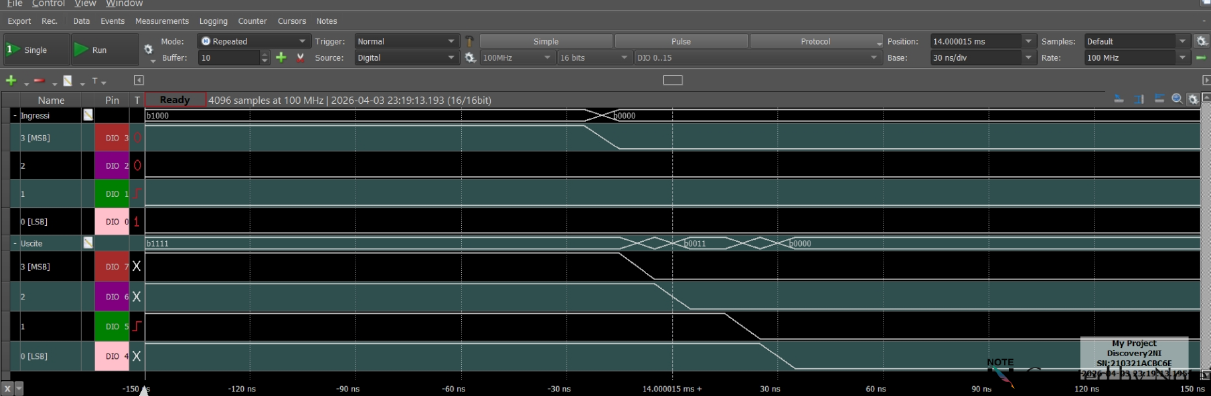
\includegraphics[width=1\linewidth]{1.png}
\end{center}

\noindent Osservando il transitorio (a cavallo di $t=14{,}000015\,\text{ms}$), è evidente come le singole linee in uscita dal blocco combinatorio scendano a zero in istanti sfalsati, generando temporaneamente un dato spuro (es. \texttt{b0011}). 
Grazie all'azione di campionamento del registro, tali irregolarità vengono confinate a monte: il circuito a valle viene aggiornato con precisione chirurgica e perfetta sincronia solo in corrispondenza del fronte di clock, garantendo un'uscita netta e priva di sfarfallii.

% ======================================================================
\chapter{Registri a scorrimento e contatori}
\textit{(17 aprile 2026)}

% ======================================================================
\section{Registri a scorrimento}

Un \textbf{registro a scorrimento} (shift register) è una catena di Flip-Flop di tipo D collegati in serie: l'uscita $Q$ di ciascuno è collegata all'ingresso $D$ del successivo. Ad ogni fronte di clock, ogni Flip-Flop «passa» il proprio valore al vicino di destra, come in un nastro trasportatore. In questo modo il dato si \emph{sposta} di una posizione ad ogni colpo di clock.

\vspace{2mm}
\noindent Per chiarire con un esempio: se il registro contiene i bit $[X, Y, Z]$ e arriva un nuovo dato $W$ dall'ingresso, dopo un tick di clock il contenuto diventa $[W, X, Y]$: il vecchio $Z$ è uscito, $X$ e $Y$ sono slittati di una posizione, e il nuovo $W$ è entrato in testa.

\subsection{Modalità di trasmissione dati}

A seconda di come si alimentano i dati in ingresso e di come si leggono in uscita, lo stesso registro fisico può funzionare in quattro modalità distinte:

\begin{itemize}[leftmargin=1.5em]
    \item \textbf{SISO} (Serial In -- Serial Out): il dato entra un bit alla volta dall'ingresso seriale ed esce un bit alla volta dall'ultimo FF. Utilizzo principale: \textbf{ritardare} un segnale digitale di esattamente $n$ cicli di clock.
    \item \textbf{SIPO} (Serial In -- Parallel Out): il dato entra un bit alla volta, ma si leggono in uscita \emph{contemporaneamente} tutti i bit memorizzati. Utilizzo tipico: convertire una trasmissione seriale (es. linea RS-232) in un dato parallelo leggibile dalla CPU.
    \item \textbf{PISO} (Parallel In -- Serial Out): si caricano tutti i bit in un solo colpo (caricamento parallelo), poi li si trasmette uno alla volta. Utilizzo: serializzare un dato parallelo per inviarlo su un bus seriale.
    \item \textbf{PIPO} (Parallel In -- Parallel Out): caricamento parallelo e lettura parallela. Funziona come un \textbf{registro di memoria}: cattura uno snapshot di un dato a $n$ bit e lo mantiene in uscita fino al prossimo aggiornamento.
\end{itemize}

\subsection{Temporizzazione e vincoli}

Affinché il registro funzioni correttamente, il clock deve rispettare due vincoli temporali critici propri di ogni Flip-Flop:

\defbox{
$T_P > T_H$, \quad $T_S + T_P < T_{CLK}$

\begin{itemize}[leftmargin=1.3em]
  \item $T_{setup}$ ($T_S$): il dato deve essere stabile sull'ingresso $D$ per almeno questo tempo \emph{prima} del fronte di clock, altrimenti non viene catturato correttamente.
  \item $T_{hold}$ ($T_H$): il dato deve rimanere stabile per almeno questo tempo \emph{dopo} il fronte di clock.
  \item $T_P$: tempo di propagazione attraverso il FF (quanto ci vuole affinché, dopo il fronte, l'uscita $Q$ si aggiorni e il nuovo valore sia pronto per il FF successivo).
  \item $I_N = D_{SR}$: dato seriale in ingresso al registro.
\end{itemize}
}

\noindent In parole semplici: il periodo del clock deve essere abbastanza lungo da permettere al segnale di attraversare il FF e di stabilizzarsi sul $D$ del successivo \emph{prima} che arrivi il fronte successivo. Se il clock è troppo veloce si leggono valori errati.

\medskip
\noindent Nei registri a scorrimento sono presenti i seguenti segnali di controllo:
\begin{itemize}[leftmargin=1.5em]
    \item \textbf{CLK}: sincronizza ogni scorrimento.
    \item \textbf{RESET/CLEAR}: azzera immediatamente l'intero registro.
    \item \textbf{SET}: forza l'uscita a $1$ (preset).
    \item \textbf{ENABLE}: quando basso, congela il registro bloccando gli scorrimenti.
\end{itemize}

\medskip
\noindent\textcolor{teal}{\textbf{Riassunto -- Differenza tra registro normale e registro a scorrimento:}}
\begin{itemize}[leftmargin=1.5em]
    \item \textbf{Registro normale (PIPO)}: cattura e conserva un dato multi-bit aggiornandolo in blocco. Non c'è scorrimento interno.
    \item \textbf{Registro a scorrimento}: conserva il dato \emph{e lo fa scorrere} di una posizione ad ogni clock, abilitando la conversione seriale$\leftrightarrow$parallelo e il ritardo digitale.
\end{itemize}

\subsection{Schemi dei registri a scorrimento (SISO, SIPO, PISO)}

Di seguito sono riportati gli schemi a blocchi semplificati per le tre configurazioni più
comuni (ogni blocco è un FF-D con uscite $Q_0$, $\overline{Q_0}$, ingresso $D$ e clock $R$/$CLK$).

\begin{fitcenter}
\begin{circuitikz}[scale=0.75, every node/.style={scale=0.75}]

% -------- PIPO --------
% 2 FF-D in cascata (rappresentativo)
\foreach \i/\xi in {0/0, 1/2.2}{
  \draw (\xi,0) rectangle (\xi+1.8, 2.2);
  \node[font=\scriptsize] at (\xi+0.9, 1.8) {${}^S$};
  \node[font=\scriptsize] at (\xi+0.4, 1.2) {$D_{\i}$};
  \node[font=\scriptsize] at (\xi+0.4, 0.7) {$Q_{\i}$};
  \node[font=\scriptsize] at (\xi+0.4, 0.3) {$\overline{Q_{\i}}$};
  \node[font=\scriptsize] at (\xi+1.4, 0.7) {$R$};
}
\draw[-latex] (-0.8, 1.2) -- (0, 1.2) node[midway,above,font=\tiny]{$D_0$};
\draw[-latex] (1.8, 0.7) -- (2.2, 0.7);
\draw[-latex] (4.0, 0.7) -- (4.6, 0.7) node[right,font=\tiny]{out};
\draw[-latex] (0.9,-0.3) -- (0.9,0) node[right,font=\tiny]{};
\draw (0.9,-0.3) -- (3.1,-0.3);
\draw[-latex] (3.1,-0.3) -- (3.1,0);
\draw (0.9,-0.3) -- (-0.4,-0.3) node[left,font=\tiny]{CLK};
\node[font=\small\bfseries] at (2.0,-0.9) {PIPO};

% -------- SISO --------
\begin{scope}[xshift=6.0cm]
\foreach \i/\xi in {0/0, 1/2.2}{
  \draw (\xi,0) rectangle (\xi+1.8, 2.2);
  \node[font=\scriptsize] at (\xi+0.9, 1.8) {${}^S$};
  \node[font=\scriptsize] at (\xi+0.4, 1.2) {$D_{\i}$};
  \node[font=\scriptsize] at (\xi+0.4, 0.7) {$Q_{\i}$};
  \node[font=\scriptsize] at (\xi+0.4, 0.3) {$\overline{Q_{\i}}$};
  \node[font=\scriptsize] at (\xi+1.4, 0.7) {$R$};
}
\draw[-latex] (-0.8,1.2) -- (0,1.2) node[midway,above,font=\tiny]{in};
\draw[-latex] (1.8,0.7) -- (2.2,1.2);
\draw[-latex] (4.0,0.7) -- (4.6,0.7) node[right,font=\tiny]{out};
\draw (0.9,-0.3) -- (-0.4,-0.3) node[left,font=\tiny]{CLK};
\draw (0.9,-0.3) -- (3.1,-0.3);
\draw[-latex] (0.9,-0.3) -- (0.9,0);
\draw[-latex] (3.1,-0.3) -- (3.1,0);
\node[font=\small\bfseries] at (2.0,-0.9) {SISO};
\end{scope}

% -------- SIPO --------
\begin{scope}[xshift=12.0cm]
\foreach \i/\xi in {0/0, 1/2.2}{
  \draw (\xi,0) rectangle (\xi+1.8, 2.2);
  \node[font=\scriptsize] at (\xi+0.9, 1.8) {${}^S$};
  \node[font=\scriptsize] at (\xi+0.4, 1.2) {$D_{\i}$};
  \node[font=\scriptsize] at (\xi+0.4, 0.7) {$Q_{\i}$};
  \node[font=\scriptsize] at (\xi+0.4, 0.3) {$\overline{Q_{\i}}$};
  \node[font=\scriptsize] at (\xi+1.4, 0.7) {$R$};
}
\draw[-latex] (-0.8,1.2) -- (0,1.2) node[midway,above,font=\tiny]{in};
\draw[-latex] (1.8,0.7) -- (2.2,1.2);
% uscite parallelo
\draw[-latex] (0.9,2.2) -- (0.9,2.7) node[above,font=\tiny]{$Q_0$};
\draw[-latex] (3.1,2.2) -- (3.1,2.7) node[above,font=\tiny]{$Q_1$};
\draw (0.9,-0.3) -- (-0.4,-0.3) node[left,font=\tiny]{CLK};
\draw (0.9,-0.3) -- (3.1,-0.3);
\draw[-latex] (0.9,-0.3) -- (0.9,0);
\draw[-latex] (3.1,-0.3) -- (3.1,0);
\node[font=\small\bfseries] at (2.0,-0.9) {SIPO};
\end{scope}

% -------- PISO --------
\begin{scope}[xshift=18.0cm]
\foreach \i/\xi in {0/0, 1/2.2}{
  \draw (\xi,0) rectangle (\xi+1.8, 2.2);
  \node[font=\scriptsize] at (\xi+0.9, 1.8) {${}^S$};
  \node[font=\scriptsize] at (\xi+0.4, 1.2) {$D_{\i}$};
  \node[font=\scriptsize] at (\xi+0.4, 0.7) {$Q_{\i}$};
  \node[font=\scriptsize] at (\xi+0.4, 0.3) {$\overline{Q_{\i}}$};
  \node[font=\scriptsize] at (\xi+1.4, 0.7) {$R$};
}
% ingressi parallelo
\draw[-latex] (0.9,2.7) -- (0.9,2.2) node[above=0.5cm,font=\tiny]{$D_0$};
\draw[-latex] (3.1,2.7) -- (3.1,2.2) node[above=0.5cm,font=\tiny]{$D_1$};
\draw[-latex] (4.0,0.7) -- (4.6,0.7) node[right,font=\tiny]{out};
\draw (0.9,-0.3) -- (-0.4,-0.3) node[left,font=\tiny]{CLK};
\draw (0.9,-0.3) -- (3.1,-0.3);
\draw[-latex] (0.9,-0.3) -- (0.9,0);
\draw[-latex] (3.1,-0.3) -- (3.1,0);
% sel
\draw[-latex] (2.2,1.8) -- (2.2,2.2) node[above,font=\tiny]{sel};
\node[font=\small\bfseries] at (2.0,-0.9) {PISO};
\end{scope}

\end{circuitikz}
\end{fitcenter}

% ======================================================================
\section{Contatori}
\textit{(17 aprile 2026)}

\defbox{
\textbf{Contatore} = circuito sequenziale che avanza automaticamente di stato ad ogni fronte di clock, rappresentando in uscita la sequenza binaria $0, 1, 2, 3, \ldots$ (o la sua inversa, nei contatori \emph{down}).
}

\noindent L'idea alla base è semplice: ogni bit dell'uscita binaria cambia a frequenza dimezzata rispetto al bit precedente.
\begin{itemize}[leftmargin=1.5em]
    \item $Q_0$ (bit meno significativo) commuta ad \textbf{ogni} periodo di clock: è il più veloce.
    \item $Q_1$ commuta ogni \textbf{2} periodi: lo fa quando $Q_0$ scende da $1$ a $0$ (fronte di discesa).
    \item $Q_{i+1}$ commuta ogni $2^{i+1}$ periodi: in generale ogni bit commuta quando il bit precedente ha un fronte di discesa.
\end{itemize}
\noindent Questo comportamento rende i contatori anche utili come \textbf{divisori di frequenza}: il clock ha frequenza $f$; $Q_0$ oscilla a $f/2$; $Q_1$ a $f/4$; e così via.

\begin{center}
\begin{tikzpicture}[scale=0.85, every node/.style={scale=0.85}]
\draw[-latex] (0,0) -- (8.0,0) node[right]{$t$};
% CLK
\draw[thick] (0,1.2) -- (0.5,1.2) -- (0.5,1.8) -- (1.0,1.8) -- (1.0,1.2) -- (1.5,1.2) -- (1.5,1.8) -- (2.0,1.8) -- (2.0,1.2) -- (2.5,1.2) -- (2.5,1.8) -- (3.0,1.8) -- (3.0,1.2) -- (3.5,1.2) -- (3.5,1.8) -- (4.0,1.8) -- (4.0,1.2) -- (7.5,1.2);
\node[right, font=\small] at (7.5,1.5) {CLK};
% Q0
\draw[thick,blue] (0,0.5) -- (1.0,0.5) -- (1.0,0.9) -- (2.0,0.9) -- (2.0,0.5) -- (3.0,0.5) -- (3.0,0.9) -- (4.0,0.9) -- (4.0,0.5) -- (7.5,0.5);
\node[right, font=\small] at (7.5,0.7) {$Q_0$};
% Q1
\draw[thick,red] (0,-0.3) -- (2.0,-0.3) -- (2.0,0.1) -- (4.0,0.1) -- (4.0,-0.3) -- (7.5,-0.3);
\node[right, font=\small] at (7.5,-0.1) {$Q_1$};
\end{tikzpicture}
\end{center}

\subsection{Contatore asincrono (ripple counter)}

Nel contatore asincrono, il clock \textbf{non arriva a tutti i Flip-Flop contemporaneamente}. Solo il primo FF riceve il clock esterno; ogni FF successivo usa come proprio clock l'uscita $\overline{Q}$ del FF precedente. In questo modo, ogni FF scatta automaticamente quando il precedente ha un fronte di discesa.

\medskip
\noindent\textcolor{teal}{\textbf{Il problema: la propagazione a catena (ripple).}} Poiché ogni FF deve aspettare che quello precedente abbia commutato, il segnale si propaga a cascata (da qui il nome \emph{ripple}). Il bit più significativo $Q_{n-1}$ non è aggiornato finché il segnale non ha attraversato tutti gli $n$ FF. Il ritardo totale vale:
\[
T_n = n \cdot T_P
\]
Questo impone che il periodo del clock sia sufficientemente lungo da permettere a tutta la catena di assestarsi prima del fronte successivo:
\[
T_{CLK} > n \cdot T_P
\]
Nei circuiti ad alta velocità questo è un limite importante: aggiungere Flip-Flop obbliga a rallentare il clock.

\begin{center}
\begin{circuitikz}[scale=0.82, every node/.style={scale=0.82}]
% 4 JK FF in cascata (asincrono)
\foreach \i/\xi in {0/0, 1/2.8, 2/5.6, 3/8.4}{
  \draw (\xi,0) rectangle (\xi+2.2, 2.0);
  \node[font=\scriptsize] at (\xi+0.55,1.5) {$K_{\i}$};
  \node[font=\scriptsize] at (\xi+0.55,1.0) {$J_{\i}$};
  \node[font=\scriptsize] at (\xi+1.7,1.0) {$Q_{\i}$};
  \node[font=\scriptsize] at (\xi+1.7,0.4) {$\overline{Q_{\i}}$};
  % J e K collegati a 1
  \draw (\xi+0.2,1.5) -- ++(-0.2,0) coordinate (K\i);
  \draw (\xi+0.2,1.0) -- ++(-0.2,0) coordinate (J\i);
}
% CLK al primo
\draw[-latex] (-1.0,1.0) -- (0,1.0) node[midway,above,font=\scriptsize]{CLK};
\node[font=\scriptsize] at (-0.7,1.8) {$1$};
\draw (-0.5,1.5) -- (0,1.5);
\draw (-0.5,1.0) -- (-0.5,1.5);
% CLK dei successivi collegato a Qi del precedente
\draw[-latex] (2.2,0.4) -- (2.8,0.4) node[midway,below,font=\scriptsize]{};
\draw[-latex] (5.0,0.4) -- (5.6,0.4);
\draw[-latex] (7.8,0.4) -- (8.4,0.4);
% uscite
\draw[-latex] (10.6,1.0) -- (11.2,1.0) node[right,font=\scriptsize]{$Q_3$};
\node[below=0.5cm, font=\small\bfseries, color=noteblue] at (5.3,-0.3) {CONTATORE ASINCRONO};
\end{circuitikz}
\end{center}

\subsection{Contatore sincrono}

Nel contatore sincrono, il clock \textbf{arriva contemporaneamente a tutti i Flip-Flop}, eliminando il ritardo a cascata e rendendo il contatore molto più veloce.

\medskip
\noindent\textbf{Come si implementa la logica di conteggio?} Non tutti i FF devono commutare ad ogni tick: $Q_1$ deve commutare solo quando $Q_0=1$; $Q_2$ solo quando $Q_0=Q_1=1$; e così via. Questa condizione viene realizzata con \textbf{porte AND in cascata}: l'ingresso $J,K$ del FF $i$-esimo è connesso all'uscita di una porta AND che combina tutti i bit $Q_0, \ldots, Q_{i-1}$. Il FF $i$ riceve il permesso di commutare solo quando tutti i bit meno significativi valgono $1$.

\begin{center}
\begin{circuitikz}[scale=0.82, every node/.style={scale=0.82}]
% 4 JK FF in parallelo sul CLK, con AND in cascata
\foreach \i/\xi in {0/0, 1/3.2, 2/6.4, 3/9.6}{
  \draw (\xi,0) rectangle (\xi+2.4, 2.2);
  \node[font=\scriptsize] at (\xi+0.6,1.7) {$K_{\i}$};
  \node[font=\scriptsize] at (\xi+0.6,1.1) {$J_{\i}$};
  \node[font=\scriptsize] at (\xi+1.85,1.1) {$Q_{\i}$};
  \node[font=\scriptsize] at (\xi+1.85,0.5) {$\overline{Q_{\i}}$};
}
% 1 su J0 e K0
\node[font=\scriptsize] at (-0.4,2.2) {$1$};
\draw[-latex] (-0.3,2.0) -- (0,2.0) -- (0,1.7);
\draw[-latex] (-0.3,2.0) -- (-0.3,1.1) -- (0,1.1);
% CLK comune
\draw[-latex] (-1.2,0.0) -- (-1.2,-0.5) -- (12.0,-0.5);
\foreach \xi in {1.2, 4.4, 7.6, 10.8}{
  \draw[-latex] (\xi,-0.5) -- (\xi,0);
}
\node[left,font=\scriptsize] at (-1.2,0) {CLK};
% AND gates tra i FF (simplified: line from Q_i to J_{i+1}/K_{i+1})
\draw[-latex] (2.4,1.1) -- (3.2,1.1);
\draw[-latex] (2.4,1.7) -- (3.2,1.7);
\draw[-latex] (5.6,1.1) -- (6.4,1.1);
\draw[-latex] (5.6,1.7) -- (6.4,1.7);
\draw[-latex] (8.8,1.1) -- (9.6,1.1);
\draw[-latex] (8.8,1.7) -- (9.6,1.7);
\draw[-latex] (12.0,1.1) -- (12.6,1.1) node[right,font=\scriptsize]{$Q_3$};

\node[below=0.5cm, font=\small\bfseries, color=noteblue] at (6.0,-0.9) {CONTATORE SINCRONO};
\end{circuitikz}
\end{center}

\subsection{Azzeramento dopo un certo conteggio (contatore modulo-M)}

Spesso non si vuole un contatore che vada da $0$ a $2^n-1$, ma che si fermi ad un numero specifico $M$ e poi riparta da zero.

\medskip
\noindent\textbf{Implementazione:} si aggiunge una porta AND ai cui ingressi arrivano le uscite $Q_i$ che sono a $1$ nella rappresentazione binaria di $M$. Non appena il contatore raggiunge $M$, l'uscita della porta AND va a $1$ e genera un segnale di \textbf{RESET asincrono} che azzera immediatamente tutti i FF riportandoli a $Q=0000$.

\medskip
\noindent\textbf{Attenzione al glitch sull'ultimo conteggio:} il valore $M$ compare realmente in uscita per un brevissimo istante (il tempo necessario affinché la porta AND lo riconosca e il reset arrivi) prima che tutto sia azzerato. L'ultimo stato ha quindi una durata anomala:
\[
T_{\text{stato }M} = T_f(\text{JK-FF}) + T_P(\text{AND})
\]

\medskip
\noindent\textbf{Esempio}: contatore modulo-6 (conta $0,1,2,3,4,5$ e poi riparte da $0$).

Quando $Q_3 Q_2 Q_1 Q_0 = 0101$ (decimale 5), la porta AND rileva questo stato e genera il RESET, riportando tutto a $0000$.

\begin{center}
\begin{circuitikz}[scale=0.82, every node/.style={scale=0.82}]
% 4 JK FF con RESET asincrono
\foreach \i/\xi in {0/0, 1/2.8, 2/5.6, 3/8.4}{
  \draw (\xi,0) rectangle (\xi+2.2, 2.0);
  \node[font=\scriptsize] at (\xi+0.55,1.5) {$K_{\i}$};
  \node[font=\scriptsize] at (\xi+0.55,1.0) {$J_{\i}$};
  \node[font=\scriptsize] at (\xi+1.7,1.0) {$Q_{\i}$};
  \node[font=\scriptsize] at (\xi+1.7,0.4) {$\overline{Q_{\i}}$};
}
% CLK
\draw[-latex] (-1.0,0.7) -- (0,0.7) node[midway,above,font=\scriptsize]{CLK};
% carry da Qi a CLK_{i+1}
\draw[-latex] (2.2,0.4) -- (2.8,0.4);
\draw[-latex] (5.0,0.4) -- (5.6,0.4);
\draw[-latex] (7.8,0.4) -- (8.4,0.4);
% AND gate per detect di 0101 -> RESET
\node[and port, scale=0.7] (AND) at (6.5,-1.2) {};
\draw (2.2,1.0) -- (2.5,1.0) |- (AND.in 1);
\draw (8.4+1.0,1.0) -- (9.8,1.0) |- (AND.in 2);
\draw (AND.out) -- ++(0.5,0) node[right,font=\scriptsize]{RESET ASINCRONO DI TUTTI i FF};
\node[font=\scriptsize] at (5.0,-1.8) {};
\end{circuitikz}
\end{center}

\subsection{Ripple Carry Output (RCO)}

I contatori binari integrati (come il classico \textbf{SN74LS163A}) includono un'uscita speciale chiamata \textbf{RCO} (Ripple Carry Output).

\medskip
\noindent\textbf{A cosa serve?} Quando si collegano più chip in cascata per formare un contatore a più bit (es. 8, 12, 16 bit), ogni chip deve segnalare al successivo quando ha terminato il proprio ciclo di conteggio. Il chip delle unità segnala al chip delle decine; il chip delle decine segnala a quello delle centinaia; e così via.

L'RCO è l'uscita di una porta NOR con 5 ingressi (i 4 $\overline{Q_i}$ e il segnale di \emph{enable}): va a $1$ per esattamente \textbf{un periodo di clock} quando il contatore ha raggiunto il valore massimo (tipicamente $Q=1111=15$). Solo in quel preciso istante tutti i $\overline{Q_i}$ sono a $0$, e la NOR dà $1$:
\[
\text{RCO} = 1 \quad \text{per un periodo } T_{CLK} \text{ quando il conteggio è al massimo.}
\]

\noindent Il chip successivo nella catena usa questo impulso RCO come \emph{enable} (o come clock) per incrementare il proprio conteggio: in questo modo si realizzano contatori a 8, 12, 16 bit collegando semplicemente chip da 4 bit in cascata tramite RCO.

\begin{center}
\begin{tikzpicture}[scale=0.85, every node/.style={scale=0.85}]
% Schema a blocchi del SN74LS163A (stilizzato)
\draw (0,0) rectangle (4.5,5.5);
\node[font=\small\bfseries] at (2.25,5.1) {SN74LS163A};
% Ingressi sincroni
\foreach \y/\lab in {4.5/CLK, 4.0/$Q_A$, 3.5/$Q_B$, 3.0/$Q_C$, 2.5/$Q_D$}{
  \draw[-latex] (-1.0,\y) -- (0,\y) node[midway,above,font=\scriptsize]{\lab};
}
% Ingressi DATA
\foreach \y/\lab in {2.0/DATA A, 1.5/DATA B, 1.0/DATA C, 0.5/DATA D}{
  \draw[-latex] (-1.2,\y) -- (0,\y) node[midway,above,font=\tiny]{\lab};
}
% Uscite
\foreach \y/\lab in {4.5/$Q_A$, 3.5/$Q_B$, 2.5/$Q_C$, 1.5/$Q_D$}{
  \draw[-latex] (4.5,\y) -- (5.5,\y) node[right,font=\scriptsize]{\lab};
}
\draw[-latex] (4.5,0.7) -- (5.5,0.7) node[right,font=\scriptsize]{RCO};
% Enable e Load
\draw[-latex] (-1.0,-0.3) -- (2.25,-0.3) -- (2.25,0) node[right,font=\tiny]{ENABLE/LOAD};
\node[font=\tiny, align=center] at (2.25,0.5) {CLOCK\\DATA INPUT};
\end{tikzpicture}
\end{center}

% ======================================================================
\chapter{Conteggio, divisori di frequenza e PRFG}
\textit{(20 aprile 2026)}

% ======================================================================
\section{Contatori a 8 bit: cascata di due SN74LS163}

Due contatori sincroni a 4 bit si collegano in \textbf{cascata} tramite il segnale RCO:
il bit più significativo (\emph{MSB}, gestito dal secondo 163) viene incrementato quando
il contatore meno significativo (\emph{LSB}) raggiunge il valore 15 e porta $\text{RCO}=1$.
Il segnale RCO del primo modulo funge da \emph{enable di conteggio} per il secondo.

\begin{center}
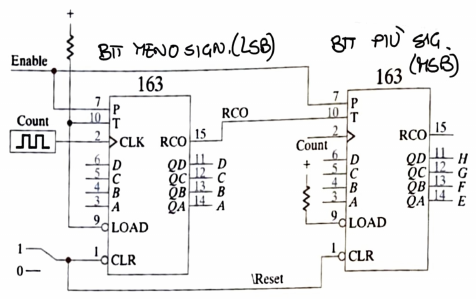
\includegraphics[width=0.85\linewidth]{img_cascata.png}
\end{center}

\noindent Due contatori sincroni a 4 bit si collegano a cascata con il RCO che funge da
\emph{enable di conteggio}: il contatore MSB avanza di un'unità ogni volta che il LSB
arriva a 15 ($\text{RCO}=1$). In questo modo si ottiene un contatore a 8 bit capace di
rappresentare i valori da 0 a 255 ($2^8-1$). Le uscite del secondo modulo ($H$, $G$, $F$,
$E$) sono i bit più significativi dell'intero conteggio; il segnale $\overline{\text{Reset}}$
asincrono è comune ad entrambi i moduli.

% ======================================================================
\section{Divisori di frequenza per un numero $n$}
\textit{(20 aprile 2026)}

\defbox{
\textbf{Divisore di frequenza} = circuito sequenziale che prende in ingresso il segnale
di clock e ne riduce la frequenza di un fattore $n$:
\[
f_{\text{out}} = \frac{f_{\text{CLK}}}{n} \qquad T_{\text{out}} = n\,T_{\text{CLK}}
\]
}

\noindent Si realizzano con il contatore SN74LS163 sfruttando il segnale RCO o il LOAD.
Esistono due varianti principali.

\subsection{Divisore con CLEAR sincrono}

Il circuito conta fino a $\text{DCBA}=1101$ (13); dopodich\'e il CLEAR \`e 1 e ricomincia
da capo.

\begin{center}
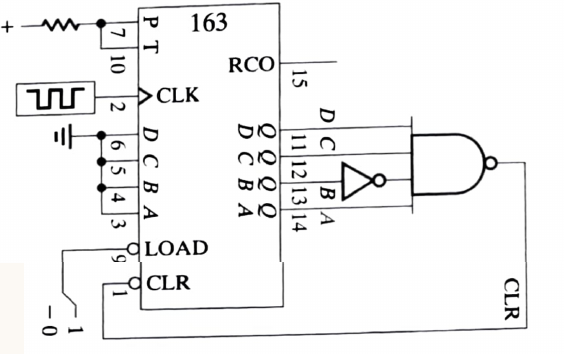
\includegraphics[width=0.52\linewidth]{img_clear.png}
\end{center}

\begin{itemize}[leftmargin=1.5em]
    \item $A$ (LSB) ha $T_A = 2\,T_{\text{CLK}}$.
    \item $D$ (MSB) ha $T_D = 16\,T_{\text{CLK}}$.
    \item Il numero 13 è l'ultimo contato, con $f = f_{\text{CLK}}/14$.
    \item Senza il clear sincrono l'ultimo stato (13) dura poco, non è esattamente un fronte.
\end{itemize}

\noindent\textit{Funzionamento}: le uscite $Q_D Q_C Q_B Q_A$ vengono decodificate da una
porta AND (con buffer invertente sul segnale $C$ per selezionare il pattern $1101$); quando
l'AND vale 1, il segnale CLR si attiva e azzera il contatore al colpo di clock successivo.
L'uscita CLR torna quindi a 0 e il ciclo ricomincia.

\subsection{Divisore con SET sincrono (LOAD)}

Il circuito ha il RCO collegato al LOAD (set) in modo che, dopo aver finito di contare,
venga caricato il valore impostato su $\text{DCBA}=0110$ (6).

\begin{center}
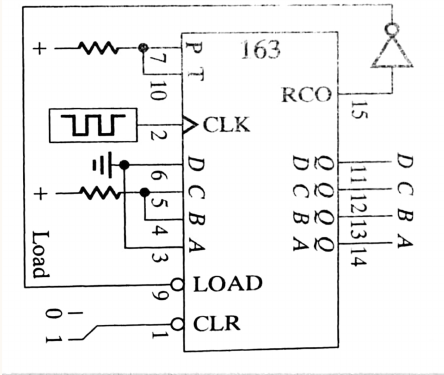
\includegraphics[width=0.52\linewidth]{img_set.png}
\end{center}

\begin{itemize}[leftmargin=1.5em]
    \item RCO ha una frequenza di $4/\text{ciclo}$ $T_{\text{CLK}}$ ($1/10$).
    \item In generale: $T_s = (2^n - n_{\text{load}})\,T_{\text{CLK}}$.
\end{itemize}

\noindent\textit{Funzionamento}: quando il contatore raggiunge 15 e $\text{RCO}=1$, al
colpo di clock successivo il LOAD forza il caricamento del valore preset ($\text{DCBA}=0110$
in questo esempio); il contatore riparte da 6 anziché da 0, ottenendo un ciclo di lunghezza
$16-6=10$, cioè $f_{\text{out}} = f_{\text{CLK}}/10$. Il LED collegato all'RCO si
accende una volta per ciclo.

% ======================================================================
\section{Contatore ad anello}

Si pone in ingresso $Q=0001$ e si applica il clock per vedere come evolve:

\[
0001 \to 0010 \to 0100 \to 1000
\]

I FF copiano il valore in entrata: contatore con solo \textbf{4 valori}.

\begin{center}
\begin{circuitikz}[scale=0.82, every node/.style={scale=0.82}]
% 4 FF-D in anello
\foreach \i/\xi in {0/0, 1/2.6, 2/5.2, 3/7.8}{
  \draw (\xi,0) rectangle (\xi+2.0,1.8);
  \node[font=\scriptsize] at (\xi+0.5,1.3) {$D_{\i}$};
  \node[font=\scriptsize] at (\xi+1.5,1.3) {$Q_{\i}$};
  \node[font=\scriptsize] at (\xi+1.5,0.5) {$\overline{Q_{\i}}$};
}
% collegamento Q_{i} -> D_{i+1}
\draw[-latex] (2.0,1.3) -- (2.6,1.3);
\draw[-latex] (4.6,1.3) -- (5.2,1.3);
\draw[-latex] (7.2,1.3) -- (7.8,1.3);
% feedback anello: Q3 -> D0
\draw (9.8,1.3) -- (9.8,2.2) -- (-0.4,2.2) -- (-0.4,1.3) -- (0,1.3);
% CLK comune
\draw[-latex] (-1.2,-0.3) -- (-1.2,-0.6) -- (9.6,-0.6);
\foreach \xi in {1.0,3.6,6.2,8.8}{
  \draw[-latex] (\xi,-0.6) -- (\xi,0);
}
\node[left,font=\scriptsize] at (-1.2,0) {CLK};
\end{circuitikz}
\end{center}

\section{Contatore ad anello \emph{twisted} (Johnson counter)}

Si pone in ingresso $Q=0000$ e si applica il clock; si nota che $\overline{Q_3}$ è
collegato a $D_0$ (feedback invertito):

\[
0000 \to 0001 \to 0011 \to 0111 \to 1111 \to 1110 \to 1100 \to 1000 \to 0000
\]

I FF copiano il valore in entrata: contatore con \textbf{8 valori} (con 4 FF).

\begin{center}
\begin{circuitikz}[scale=0.82, every node/.style={scale=0.82}]
% 4 FF-D in anello twisted
\foreach \i/\xi in {0/0, 1/2.6, 2/5.2, 3/7.8}{
  \draw (\xi,0) rectangle (\xi+2.0,1.8);
  \node[font=\scriptsize] at (\xi+0.5,1.3) {$D_{\i}$};
  \node[font=\scriptsize] at (\xi+1.5,1.3) {$Q_{\i}$};
  \node[font=\scriptsize] at (\xi+1.5,0.5) {$\overline{Q_{\i}}$};
}
% collegamento Q_{i} -> D_{i+1}
\draw[-latex] (2.0,1.3) -- (2.6,1.3);
\draw[-latex] (4.6,1.3) -- (5.2,1.3);
\draw[-latex] (7.2,1.3) -- (7.8,1.3);
% feedback twisted: Qbar_3 -> D0
\draw (9.8,0.5) -- (9.8,-0.9) -- (-0.4,-0.9) -- (-0.4,1.3) -- (0,1.3);
\node[font=\scriptsize] at (10.3,0.5) {$\overline{Q_3}$};
% CLK comune
\draw[-latex] (-1.2,0.9) -- (0,0.9);
\foreach \xi in {2.6,5.2,7.8}{
  \draw[-latex] (\xi-0.3,0.9) -- (\xi,0.9);
}
\node[left,font=\scriptsize] at (-1.2,0.9) {CLK};
\end{circuitikz}
\end{center}

\defbox{
Rispetto al contatore ad anello normale, il Johnson counter ha \textbf{2N stati} per N
flip-flop utilizzati per realizzarlo.
}

% ======================================================================
\section{Generatori di frequenza pseudo casuali (PRFG)}

\defbox{
\textbf{PRFG} (\emph{Pseudo-Random Frequency Generator}) = applicazione dei registri a
scorrimento che ha trovato grande applicazione nella generazione di sequenze di bit pseudo
casuali. Il registro ha grandezza fissa; questo comporta lo ``pseudo''.\\[0.3em]
Un registro largo $K$ FF genera una sequenza ripetuta al massimo dopo $2^K-1$ eventi.
}

\noindent Nei generatori pseudo casuali \textbf{lineari} si usa lo XOR (o XNOR) per
costruire il circuito: le porte equivalenti alla somma binaria.

\defbox{
\textbf{LPRG} = \emph{Linear Pseudo Random Generator}
}

\begin{center}
\begin{circuitikz}[scale=0.82, every node/.style={scale=0.82}]
% 4 FF-D con feedback XOR (LFSR)
\foreach \i/\xi in {0/0, 1/2.6, 2/5.2, 3/7.8}{
  \draw (\xi,0) rectangle (\xi+2.0,1.8);
  \node[font=\scriptsize] at (\xi+0.5,1.3) {$D_{\i}$};
  \node[font=\scriptsize] at (\xi+1.5,1.3) {$Q_{\i}$};
  \node[font=\scriptsize] at (\xi+1.5,0.5) {$\overline{Q_{\i}}$};
}
% shift: Q_{i} -> D_{i+1}
\draw[-latex] (2.0,1.3) -- (2.6,1.3);
\draw[-latex] (4.6,1.3) -- (5.2,1.3);
\draw[-latex] (7.2,1.3) -- (7.8,1.3);
% XOR gate per feedback
\node[xor port, scale=0.7] (XF) at (1.3, 3.0) {};
% Q3 -> XOR in1 (feedback)
\draw (9.8,1.3) -- (9.8,3.0) -- (XF.in 1);
% Q0 (o altro tap) -> XOR in2
\draw (2.0,1.3) -- (2.0,2.4) -- (XF.in 2);
% XOR out -> D0
\draw[-latex] (XF.out) -- (0,3.0) -- (0,1.8);
% CLK comune
\draw[-latex] (-1.2,-0.4) -- (-1.2,-0.7) -- (9.6,-0.7);
\foreach \xi in {1.0,3.6,6.2,8.8}{
  \draw[-latex] (\xi,-0.7) -- (\xi,0);
}
\node[left,font=\scriptsize] at (-1.2,0) {CLK};
\end{circuitikz}
\end{center}

\noindent La tabella degli stati del LPRG a 3 FF (FF0, FF1, FF2), con feedback XOR tra
FF2 e FF1, mostra la sequenza pseudo casuale di lunghezza $2^3-1=7$:

\begin{center}
\begin{tabular}{c|ccc}
\toprule
Clock & FF0 & FF1 & FF2 \\
\midrule
0 & 1 & 1 & 1 \\
1 & 0 & 1 & 1 \\
2 & 1 & 0 & 1 \\
3 & 1 & 1 & 0 \\
4 & 0 & 1 & 1 \\
5 & 1 & 0 & 1 \\
6 & 0 & 0 & 1 \\
7 & 1 & 0 & 0 \\
8 & 1 & 1 & 0 \\
9 & 0 & 1 & 1 \\
10 & 0 & 0 & 1 \\
11 & 1 & 0 & 0 \\
12 & 1 & 1 & 0 \\
13 & 1 & 1 & 1 \\
\bottomrule
\end{tabular}
\end{center}

% ======================================================================
\chapter{Macchine a stati finiti (FSM)}
\textit{(24 aprile 2026)}

\defbox{
\textbf{FSM} (\emph{Finite State Machine}) = architettura in cui gli stati presenti
determinano quelli futuri.
}

\defbox{
\textbf{Diagramma di stato} = mappa per rappresentare il comportamento di un sistema
sequenziale (possibili stati e legami).\\[0.3em]
Gli stati sono legati fra loro da precise transizioni. Gli stati sono definiti da
condizioni \textbf{INTERNE} (presenti nel sistema) e/o da condizioni \textbf{ESTERNE}
(segnali in ingresso dall'esterno).
}

\noindent Ogni circuito digitale è una FSM.

% ======================================================================
% Continuazione Capitolo 8: Macchine a stati finiti (FSM)
% (24 aprile 2026)
% ======================================================================

\section{Tipi di architettura FSM: Moore e Mealy}

Esistono due tipi principali di architettura per le FSM:

\begin{itemize}[leftmargin=1.5em]
    \item \textbf{Architettura di Moore}
    \item \textbf{Architettura di Mealy}
\end{itemize}

\subsection{Architettura di Moore}

\begin{center}
\begin{tikzpicture}[scale=0.85, every node/.style={scale=0.85},
  box/.style={draw, minimum width=2.0cm, minimum height=1.0cm, align=center, font=\small}]

\node[box] (lcf) at (0,0)    {logica\\combinatoria\\stato futuro};
\node[box] (reg) at (3.6,0)  {registro\\di\\memoria};
\node[box] (lcu) at (7.2,0)  {logica\\combinatoria\\uscite};

% Frecce principali
\draw[-latex] (-1.8,0) -- (lcf.west) node[midway,above,font=\scriptsize]{ingressi};
\draw[-latex] (lcf.east) -- (reg.west) node[midway,above,font=\scriptsize]{futuro};
\draw[-latex] (reg.east) -- (lcu.west) node[midway,above,font=\scriptsize]{presente};
\draw[-latex] (lcu.east) -- ++(1.4,0) node[right,font=\scriptsize]{uscite};

% CLK al registro
\draw[-latex] (3.6,-1.2) -- (reg.south) node[below=1.0cm,font=\scriptsize]{CLK};

% Feedback dallo stato presente alla logica combinatoria stato futuro
\draw[-latex] (3.6,0.5) -- (3.6,1.4) -- (-0.2,1.4) -- (-0.2,0.5);

% bus (freccia dal basso dell'uscita)
\draw[-latex] (8.0,-0.5) -- (8.0,-1.2) node[below,font=\scriptsize]{bus};

\end{tikzpicture}
\end{center}

\begin{itemize}[leftmargin=1.5em]
    \item Uno stato è univocamente conseguenza dello stato precedente.
    \item Gli ingressi esterni non sempre sono presenti.
\end{itemize}

% ======================================================================
\section{Dal diagramma di stato al circuito}
\textit{(24 aprile 2026)}

\noindent Il diagramma di stato è composto da \textbf{stati} (cerchi etichettati con il
valore di uscita) collegati da \textbf{transizioni} (frecce etichettate con il valore
dell'ingresso/condizione):

\begin{center}
\begin{tikzpicture}[scale=0.9, every node/.style={scale=0.9},
  state/.style={draw, circle, minimum size=1.0cm, font=\small, align=center}]

\node[state] (s0) at (0,0)    {$S_0$ \\ {\tiny 00}};
\node[state] (s1) at (2.4,-1.2)  {$S_1$ \\ {\tiny 011}};
\node[state] (s2) at (-2.4,-1.2) {$S_2$ \\ {\tiny 101}};

\draw[-latex] (s0) -- (s1);
\draw[-latex] (s1) -- (s2);
\draw[-latex] (s2) -- (s0);

\node[above right, font=\scriptsize] at (s0.north east) {stato};
\node[below, font=\scriptsize] at (s1.south) {valore di uscita};
\node[left,  font=\scriptsize] at (-1.5,-1.8) {transizione};
\node[above, font=\scriptsize, color=noteteal] at (0.6,-0.4) {diagramma di stato};

\end{tikzpicture}
\end{center}

\noindent La procedura per passare dal diagramma di stato al circuito è la seguente:

\begin{enumerate}[leftmargin=1.5em]
    \item \textbf{Dato il numero di stati} (3) definisco il numero di bit che mi serve a
          rappresentarli: $\lceil\log_2 3\rceil = 2\;\Rightarrow\;$ 2 bit.
    \item \textbf{Associo a ogni stato una rappresentazione in bit}:
          $S_0=[00]$, $S_1=[01]$, $S_2=[10]$, $S_3=[X]$ \emph{(don't care)}.
    \item \textbf{Per ogni bit uso un FF}: $S_i = Q_i Q_0^i$.
    \item \textbf{Scrivo la tabella di verità}: associo a ogni stato presente uno stato
          futuro.

\begin{center}
\begin{tabular}{cc|cc}
\toprule
$Q_1$ & $Q_0$ & $Q_1^+$ & $Q_0^+$\\
\midrule
0 & 0 & 0 & 1\\
0 & 1 & 1 & 0\\
1 & 0 & 0 & 0\\
1 & 1 & $\times$ & $\times$\\
\bottomrule
\end{tabular}
\end{center}

    \item \textbf{Scelgo il tipo di FF} (D, JK, T): in questo caso uso DFF,
          poiché $Q^+=D$.
    \item \textbf{Ricavo le funzioni di $D_i = f(Q_i)$}:
          \[
          D_1 = Q_0 \qquad D_0 = \overline{Q_1}\cdot\overline{Q_0}
          \]
    \item \textbf{Disegno il circuito}:

\begin{center}
\begin{circuitikz}[scale=0.85, every node/.style={scale=0.85}]
% Due DFF in cascata
\draw (0,0) rectangle (1.8,2.0);
\node[font=\scriptsize] at (0.5,1.5) {$D_0\,Q_0$};
\node[font=\scriptsize] at (0.5,0.5) {$\overline{Q_0}$};
\draw (2.8,0) rectangle (4.6,2.0);
\node[font=\scriptsize] at (3.3,1.5) {$D_1\,Q_1$};
\node[font=\scriptsize] at (3.3,0.5) {$\overline{Q_1}$};

% D0 <- feedback da Q0 (D0 = Qbar1 * Qbar0, semplificato come segnale)
\draw[-latex] (-1.0,1.5) -- (0,1.5) node[midway,above,font=\tiny]{$D_0$};
% Q0 -> D1
\draw[-latex] (1.8,1.5) -- (2.8,1.5) node[midway,above,font=\tiny]{$Q_0$};
% Uscita Q1
\draw[-latex] (4.6,1.5) -- (5.4,1.5) node[right,font=\tiny]{$Q_1$};

% CLK comune
\draw[-latex] (-1.0,-0.5) -- (0.9,-0.5) -- (0.9,0) node[above,font=\tiny]{};
\draw (0.9,-0.5) -- (3.7,-0.5);
\draw[-latex] (3.7,-0.5) -- (3.7,0);
\node[left,font=\scriptsize] at (-1.0,-0.5) {CLK};
\end{circuitikz}
\end{center}

\end{enumerate}

\defbox{
\begin{itemize}[leftmargin=1.3em,itemsep=2pt]
    \item \textbf{DFF}: $Q^+=D$ \quad più usato, semplice.
    \item \textbf{TFF}: $Q^+=T\oplus Q$ \quad per contatori e sequenze regolari.
    \item \textbf{JKFF}: flessibile, può fare tutto (set, reset, toggle).
\end{itemize}
}

\subsection{Ricavare le funzioni dei segnali di uscita: $O_i = f(Q_i)$}

\begin{center}
\begin{tabular}{cc|cc|ccc}
\toprule
$Q_1$ & $Q_0$ & $D_0$ & $D_1$ & $O_2$ & $O_1$ & $O_0$\\
\midrule
0 & 0 & 1 & 0 & 0 & 1 & 0\\
0 & 1 & 0 & 1 & 0 & 1 & 1\\
1 & 0 & 0 & 0 & 1 & 0 & 1\\
1 & 1 & $\times$ & $\times$ & $\times$ & $\times$ & $\times$\\
\bottomrule
\end{tabular}
\end{center}

\[
O_0 = Q_0 + Q_1 \qquad O_1 = \overline{Q_1} \qquad O_2 = Q_1
\]

\subsection{Stato bloccante e segnale di Enable}

Al punto 9 si verifica quale sia lo stato futuro del caso $Q_1 = Q_0 = 1$: se è uno
\textbf{stato bloccante}, è un problema che dobbiamo risolvere.

\noindent Nel nostro caso, da $Q=11$ si andrà a finire in $D=10$, quindi ricomincerà la
sequenza (non blocca il circuito).

\medskip
\noindent Se volessimo scorrere il ciclo al contrario, possiamo inserire un segnale di
\textbf{Enable}:

\begin{itemize}[leftmargin=1.5em]
    \item $E=1$: si ha $010 \to 011 \to 101$ \quad (dritto).
    \item $E=0$: si ha $101 \to 011 \to 010$ \quad (rovescio).
\end{itemize}

\noindent Cambiamo le entrate $D_i$ ma le uscite restano le stesse:
\[
D_i = f(Q_i, E) \qquad O_i = f(Q_i)
\]

\noindent Possiamo scrivere le funzioni:
\[
D_1 = \overline{E}\cdot\overline{Q_1}\cdot\overline{Q_0} + E\cdot Q_0
\qquad
D_0 = E\cdot\overline{Q_1}\cdot\overline{Q_0} + \overline{E}\cdot Q_1
\]

\begin{center}
\begin{tikzpicture}[scale=0.85, every node/.style={scale=0.85},
  state/.style={draw, circle, minimum size=0.9cm, font=\scriptsize, align=center}]

% Diagramma di stato con Enable
\node[state] (s0) at (0,0)       {$S_0$ \\ {\tiny 00}};
\node[state] (s1) at (2.2,-1.0)  {$S_1$ \\ {\tiny 011}};
\node[state] (s2) at (-2.2,-1.0) {$S_2$ \\ {\tiny 101}};

\draw[-latex,bend left=15] (s0) to (s1);
\draw[-latex,bend left=15] (s1) to (s2);
\draw[-latex,bend left=15] (s2) to (s0);

\end{tikzpicture}
\hspace{1.5cm}
\begin{circuitikz}[scale=0.82, every node/.style={scale=0.82}]
% Schema a blocchi con Enable
\draw (1.5,0) rectangle (3.3,2.2);
\node[font=\scriptsize] at (2.1,1.7) {$D_0\,Q_0$};
\node[font=\scriptsize] at (2.1,0.5) {$\overline{Q_0}$};

\draw (4.2,0) rectangle (6.0,2.2);
\node[font=\scriptsize] at (4.8,1.7) {$D_1\,Q_1$};
\node[font=\scriptsize] at (4.8,0.5) {$\overline{Q_1}$};

% E entra nella logica a sinistra
\draw[-latex] (0.0,1.7) -- (1.5,1.7) node[midway,above,font=\tiny]{$D_0$};
\draw[-latex] (-0.5,2.5) -- (0.8,2.5) -- (0.8,1.7) node[near start,above,font=\tiny]{$E$};

% Q0 -> D1
\draw[-latex] (3.3,1.7) -- (4.2,1.7);
% Uscite
\draw[-latex] (6.0,1.7) -- (6.8,1.7) node[right,font=\tiny]{$Q_1$};

% CLK
\draw[-latex] (0.2,-0.9) -- (2.4,-0.9) -- (2.4,0);
\draw (2.4,-0.9) -- (5.1,-0.9);
\draw[-latex] (5.1,-0.9) -- (5.1,0);
\node[left,font=\scriptsize] at (0.2,-0.9) {CLK};

% Label logiche
\node[below=0.3cm,font=\scriptsize,align=center,color=noteteal] at (0.7,0)
      {logica che mi permette\\di ottenere $D_i=f(Q_i,E)$};
\node[below=0.3cm,font=\scriptsize,align=center,color=noteteal] at (6.5,0)
      {logica che permette\\di ottenere $O_i=f(Q_i)$};
\end{circuitikz}
\end{center}

% ======================================================================
% Seguito Capitolo 8 -- Macchine a stati finiti (FSM)
% Continuazione esempio insegna luminosa + Architettura di Mealy
% (27 aprile 2026)
% ======================================================================

\subsection{Esempio: insegna luminosa (continuazione)}

La sequenza dell'insegna luminosa, con $E=1$, è:
\[
RABA \to RABS \to RSBA \to RABA \to \cdots \quad (E=1)
\]
\[
BA \to BS \to BA \to \cdots \quad (E=0, \text{ RS costante})
\]

\noindent Per aggiungere lo stato ``$RS$ costante'' disabilitato, dobbiamo aggiungere un
4\textdegree{} stato, perché $O_i \leftrightarrow f(Q_i) \not\ni E$.

\begin{center}
\begin{tikzpicture}[scale=0.88, every node/.style={scale=0.88},
  state/.style={draw, circle, minimum size=1.1cm, font=\scriptsize, align=center}]

% Diagramma Moore (sinistra)
\node[state] (s0M) at (0, 2.0) {$S_0$\\{[RB]}};
\node[state] (s1M) at (-1.4, 0) {$S_1$\\{[R]}};
\node[state] (s2M) at (1.4, 0)  {$S_2$\\{[B]}};

\draw[-latex, dashed, bend left=15] (s0M) to node[right,font=\tiny]{R} (s1M);
\draw[-latex, dashed, bend left=15] (s1M) to node[below,font=\tiny]{B} (s2M);
\draw[-latex, dashed, bend left=15] (s2M) to node[right,font=\tiny]{} (s0M);
\draw[-latex] (s0M) to[bend right=30] node[left,font=\tiny]{} (s1M);

\node[font=\small\bfseries] at (0,-1.0) {Moore};

% Diagramma Mealy (destra) con stato S3 disabilitato
\begin{scope}[xshift=5.5cm]
\node[state] (s0) at (0, 2.0) {$S_0$\\{[RB]}};
\node[state] (s1) at (-1.4, 0) {$S_1$\\{[R]}};
\node[state] (s2) at (1.4, 0)  {$S_2$\\{[B]}};
\node[state] (s3) at (1.4,-1.6) {$S_3$\\{[-]}};

\draw[-latex, dashed, bend left=15] (s0) to (s1);
\draw[-latex, dashed, bend left=15] (s1) to (s2);
\draw[-latex, dashed, bend left=15] (s2) to (s0);
% S3 con E=0+1
\draw[-latex] (s3) to[bend left=20] (s2);
\node[right, font=\scriptsize, color=noteteal] at (2.0,-0.8) {$E\!=\!0\!+\!1$};

\node[font=\small\bfseries] at (0,-2.4) {Mealy};
\end{scope}

\end{tikzpicture}
\end{center}

\noindent Possiamo quindi implementare l'architettura di Moore.

% ======================================================================
\section{Architettura di Mealy}
\textit{(27 aprile 2026)}

\begin{center}
\begin{tikzpicture}[scale=0.85, every node/.style={scale=0.85},
  box/.style={draw, minimum width=2.0cm, minimum height=1.0cm, align=center, font=\small}]

\node[box] (lcf) at (0,0)   {logica\\combinatoria\\stato futuro};
\node[box] (reg) at (3.6,0) {registro\\di\\memoria};
\node[box] (lcu) at (7.2,0) {logica\\combinatoria\\uscite};

\draw[-latex] (-2.0,0) -- (lcf.west) node[midway,above,font=\scriptsize]{ingressi};
\draw[-latex] (lcf.east) -- (reg.west) node[midway,above,font=\scriptsize]{futuro};
\draw[-latex] (reg.east) -- (lcu.west) node[midway,above,font=\scriptsize]{presente};
\draw[-latex] (lcu.east) -- ++(1.4,0) node[right,font=\scriptsize]{uscite};

% CLK
\draw[-latex] (3.6,-1.2) -- (reg.south) node[below=1.0cm,font=\scriptsize]{CLK};

% Feedback: stato presente -> logica stato futuro
\draw[-latex] (3.6, 0.5) -- (3.6,1.4) -- (-0.2,1.4) -- (-0.2,0.5);

% Differenza: ingressi vanno anche alla logica uscite (linea tratteggiata)
\draw[-latex, dashed] (-1.4,0) -- (-1.4,-1.0) -- (7.2,-1.0) -- (7.2,-0.5);

\end{tikzpicture}
\end{center}

\noindent La differenza principale fra Moore e Mealy è la dipendenza delle uscite dai
parametri del circuito:
\begin{itemize}[leftmargin=1.5em]
    \item in \textbf{Moore}: $O_i = f(Q_i)$, sincrona al clock.
    \item in \textbf{Mealy}: $O_i = f(Q_i, I_i)$, asincrona.
\end{itemize}

\noindent Il valore delle uscite si associa alle \textbf{transizioni}. Riprendendo l'esempio
dell'insegna luminosa, il diagramma di Mealy è:

\begin{center}
\begin{tikzpicture}[scale=0.9, every node/.style={scale=0.9},
  state/.style={draw, circle, minimum size=1.0cm, font=\scriptsize, align=center}]

\node[state] (s0) at (0,0)    {$S_0$\\{\tiny 00}};
\node[state] (s1) at (-2.0,-1.6) {$S_1$\\{\tiny 01}};
\node[state] (s2) at (2.0,-1.6)  {$S_2$\\{\tiny 10}};

% Transizioni con etichette RB, R, B
\draw[-latex, bend left=10] (s0) to node[left, font=\scriptsize]{$-$} (s1);
\draw[-latex, bend left=10] (s1) to node[below, font=\scriptsize]{B} (s2);
\draw[-latex, bend left=10] (s2) to node[right, font=\scriptsize]{R} (s0);
\draw[-latex] (s0) to[loop above] node[font=\scriptsize]{RB} (s0);

% Ingressi E su transizioni
\node[above left, font=\tiny] at (-0.4, -0.6) {$RB$};

\end{tikzpicture}
\end{center}

\begin{itemize}[leftmargin=1.5em]
    \item $E=1$: l'uscita è legata al passaggio fra 2 stati, non allo stato di per sé.
    \item $E=0$: il fronte di clock è asincrono, perché dipende anche da $E$, che è
          asincrono: se il clock si ferma ma $E$ cambia, allora le uscite cambiano.
\end{itemize}

\noindent Per implementare il circuito dei registri si usano JKFF in modalità
``\textbf{toggle}'' (1) oppure ``\textbf{hold}'' (0): $J=K$ in una sola modalità.

\subsection{Tabella di verità dell'insegna luminosa (Mealy)}

\begin{center}
\begin{tabular}{cc|cc|cc}
\toprule
\multicolumn{2}{c|}{} & \multicolumn{2}{c|}{stato futuro} & \multicolumn{2}{c}{uscite}\\
$Q_1$ & $Q_0$ & $Q_1^+$ & $Q_0^+$ & $R$ & $B$\\
\midrule
\multicolumn{6}{l}{$E=1$}\\
\midrule
0 & 0 & 0 & 1 & 1 & 1\\
0 & 1 & 1 & 0 & 1 & 0\\
1 & 0 & 0 & 0 & 0 & 1\\
1 & 1 & $\times$ & $\times$ & $\times$ & $\times$\\
\midrule
\multicolumn{6}{l}{$E=0$}\\
\midrule
0 & 0 & 0 & 0 & 1 & 0\\
0 & 1 & 0 & 1 & 0 & 1\\
1 & 0 & 0 & 1 & 0 & 1\\% [DA VERIFICARE: riga 1,0 con E=0 — leggibile come Q+=01]
1 & 1 & $\times$ & $\times$ & $\times$ & $\times$\\
\bottomrule
\end{tabular}
\end{center}

\subsection{Tabella JK per l'implementazione}

Usando JKFF con $J=K$ (modalità toggle quando $Q_i \neq Q_i^+$, hold quando $Q_i = Q_i^+$):

\begin{center}
\begin{tabular}{cc|cc|cc}
\toprule
$Q_1$ & $Q_0$ & $Q_1^+$ & $Q_0^+$ & $JK_1$ & $JK_0$\\
\midrule
\multicolumn{6}{l}{$E=1$}\\
\midrule
0 & 0 & 0 & 1 & 0 & 1\\
0 & 1 & 1 & 0 & 1 & 1\\
1 & 0 & 0 & 0 & 1 & 0\\
1 & 1 & $\times$ & $\times$ & $\times$ & $\times$\\
\midrule
\multicolumn{6}{l}{$E=0$}\\
\midrule
0 & 0 & 0 & 0 & 0 & 0\\% hold su entrambi
0 & 1 & 0 & 1 & 0 & 0\\
1 & 0 & 0 & 1 & 1 & 1\\
1 & 1 & $\times$ & $\times$ & $\times$ & $\times$\\
\bottomrule
\end{tabular}
\end{center}

\begin{itemize}[leftmargin=1.5em]
    \item Quando $Q_i = Q_i^+$: fa \textbf{hold} ($JK=0$).
    \item Quando $\overline{Q_i} = Q_i^+$: fa \textbf{toggle} ($JK=1$).
\end{itemize}

\[
Q_1^+ = E\,Q_0 \qquad\qquad Q_0^+ = \overline{Q_0}\,(\overline{E}+\overline{Q_1})
\]

\subsection{Mappe di Karnaugh per $JK_0$ e $JK_1$}

\begin{fitcenter}
\begin{tikzpicture}[scale=0.82, every node/.style={scale=0.82}]

% --- Mappa JK0 ---
\node[font=\small] at (2.0,3.2) {Mappa $JK_0$};
\draw (0,0) grid (4,2);
% header colonne Gray: Q1Q0 = 00, 01, 11, 10
\node[font=\scriptsize] at (0.5,2.35) {00};
\node[font=\scriptsize] at (1.5,2.35) {01};
\node[font=\scriptsize] at (2.5,2.35) {11};
\node[font=\scriptsize] at (3.5,2.35) {10};
\node[font=\scriptsize, anchor=east] at (-0.1,1.5) {0};
\node[font=\scriptsize, anchor=east] at (-0.1,0.5) {1};
\node[font=\scriptsize] at (-0.7,2.35) {$E\backslash Q_1Q_0$};
% Valori: riga E=0: 0,0,X,0; riga E=1: 1,1,X,0
\node at (0.5,1.5) {0}; \node at (1.5,1.5) {0}; \node at (2.5,1.5) {$\times$}; \node at (3.5,1.5) {0};
\node at (0.5,0.5) {1}; \node at (1.5,0.5) {1}; \node at (2.5,0.5) {$\times$}; \node at (3.5,0.5) {0};
% Raggruppamento (viola): celle (E=1,00),(E=1,01) + (E=0... non incluse)
\draw[violet, thick, rounded corners=3pt] (0.06,0.06) rectangle (1.94,0.94);
% Raggruppamento esteso con don't care
\draw[violet, thick, rounded corners=3pt] (0.06,0.06) rectangle (2.94,1.94);
% Label risultato
\node[fill=yellow!40, rounded corners=2pt, font=\small] at (5.4,0.5)
      {$JK_0=\overline{Q_1}+\overline{E}$};

% --- Mappa JK1 ---
\begin{scope}[xshift=7.5cm]
\node[font=\small] at (2.0,3.2) {Mappa $JK_1$};
\draw (0,0) grid (4,2);
\node[font=\scriptsize] at (0.5,2.35) {00};
\node[font=\scriptsize] at (1.5,2.35) {01};
\node[font=\scriptsize] at (2.5,2.35) {11};
\node[font=\scriptsize] at (3.5,2.35) {10};
\node[font=\scriptsize, anchor=east] at (-0.1,1.5) {0};
\node[font=\scriptsize, anchor=east] at (-0.1,0.5) {1};
\node[font=\scriptsize] at (-0.7,2.35) {$E\backslash Q_1Q_0$};
% Valori: riga E=0: 0,0,X,1; riga E=1: 0,1,X,1
\node at (0.5,1.5) {0}; \node at (1.5,1.5) {0}; \node at (2.5,1.5) {$\times$}; \node at (3.5,1.5) {1};
\node at (0.5,0.5) {0}; \node at (1.5,0.5) {1}; \node at (2.5,0.5) {$\times$}; \node at (3.5,0.5) {1};
% Raggruppamenti
\draw[teal, thick, rounded corners=3pt] (1.06,0.06) rectangle (2.94,0.94);
\draw[orange!80!black, thick, rounded corners=3pt] (2.06,0.06) rectangle (3.94,1.94);
\node[fill=orange!30, rounded corners=2pt, font=\small] at (5.6,0.5)
      {$JK_1=Q_1+E\,Q_0$};
\end{scope}

\end{tikzpicture}
\end{fitcenter}

% ======================================================================
\section{Esempio: riconoscitore di sequenze}

In ingresso c'è una serie di bit: vogliamo accendere un LED quando trovo $Q_{i+1}Q_i=11$:

\medskip
\noindent Serie di bit: $I = 1011010\mathbf{11}10001\ldots$ \quad \textbf{LED acceso}

\begin{itemize}[leftmargin=1.5em]
    \item $S_0$ = non ho ancora trovato il $1^\circ$ $1$: LED spento (S).
    \item $S_1$ = ho trovato il $1^\circ$ $1$: LED spento (S).
    \item $S_2$ = ho trovato il $2^\circ$ $1$: LED acceso (A).
    \item $I=1$, $I=0$.
\end{itemize}

\begin{center}
\begin{tikzpicture}[scale=0.88, every node/.style={scale=0.88},
  state/.style={draw, circle, minimum size=1.1cm, font=\scriptsize, align=center}]

% Moore
\node[state] (m0) at (0,0)    {$S_0$\\{\tiny [00]}};
\node[state] (m1) at (2.4,0)  {$S_1$\\{\tiny [01]}};
\node[state] (m2) at (1.2,-1.8) {$S_2$\\{\tiny [11]}};

\draw[-latex] (m0) to[bend left=20] node[above,font=\tiny]{$I\!=\!1$} (m1);
\draw[-latex] (m0) to[loop left]    node[font=\tiny]{$I\!=\!0$} (m0);
\draw[-latex] (m1) to[bend left=20] node[left,font=\tiny]{$I\!=\!1$} (m2);
\draw[-latex] (m1) to[bend left=20] node[below,font=\tiny]{$I\!=\!0$} (m0);
\draw[-latex] (m2) to[loop below]   node[font=\tiny]{$I\!=\!1$} (m2);
\draw[-latex] (m2) to[bend left=20] node[right,font=\tiny]{$I\!=\!0$} (m0);

\node[font=\small\bfseries] at (1.2,-2.8) {Moore};

% Mealy
\begin{scope}[xshift=6.0cm]
\node[state] (my0) at (0,0)   {$S_0$};
\node[state] (my1) at (2.4,0) {$S_1$};

\draw[-latex] (my0) to[bend left=20] node[above,font=\tiny]{$I\!=\!1$/LS} (my1);
\draw[-latex] (my0) to[loop left]    node[font=\tiny]{$I\!=\!0$/LS} (my0);
\draw[-latex] (my1) to[loop right]   node[font=\tiny]{$I\!=\!1$/LS} (my1);
\draw[-latex] (my1) to[bend left=20] node[below,font=\tiny]{$I\!=\!0$/LA} (my0);

\node[font=\small\bfseries] at (1.2,-1.6) {Mealy};
\end{scope}

\end{tikzpicture}
\end{center}

% ======================================================================
\section{Esempio: macchina distributrice del caffè}

\begin{itemize}[leftmargin=1.5em]
    \item Costo caffè: $0{,}30\,\text{€}$.
    \item L'erogazione del caffè avviene se metto $\geq 0{,}30\,\text{€}$.
    \item La macchina \textbf{non dà resto}.
    \item La macchina riconosce il peso e accetta solo monete da $0{,}10\,\text{€}$
          e $0{,}20\,\text{€}$.
\end{itemize}

\noindent Stati della macchina (2 FF, 4 stati):

\begin{center}
\begin{tabular}{ll}
\toprule
Stato & Credito\\
\midrule
$S_0$ & $0\,\text{cent}$\\
$S_1$ & $10\,\text{cent}$\\
$S_2$ & $20\,\text{cent}$\\
$S_3$ & $\geq 30\,\text{cent}$\\
\bottomrule
\end{tabular}
\end{center}

% ======================================================================
% Seguito Capitolo 8 -- completamento macchina caffè
% ======================================================================

\subsection{Diagramma di stato della macchina del caffè (Moore)}

\noindent Per Mealy ogni stato non deve avere uscite mai definite, altrimenti
ci sono dei problemi di confusione.

\begin{center}
\begin{tikzpicture}[scale=0.9, every node/.style={scale=0.9},
  state/.style={draw, circle, minimum size=1.1cm, font=\scriptsize, align=center}]

\node[state] (s0) at (0, 2.2)   {$S_0$\\{\tiny [0]}};
\node[state] (s1) at (-2.4, 0)  {$S_1$\\{\tiny [10]}};
\node[state] (s2) at (2.4, 0)   {$S_2$\\{\tiny [20]}};
\node[state] (s3) at (0, -2.0)  {$S_3$\\{\tiny [30]}};

% S0 self-loop (0 cent inseriti)
\draw[-latex] (s0) to[loop above] node[font=\scriptsize]{0} (s0);
% S0 -> S1 con 10
\draw[-latex] (s0) to[bend right=15] node[left,  font=\scriptsize]{10} (s1);
% S0 -> S2 con 20
\draw[-latex] (s0) to[bend left=15]  node[right, font=\scriptsize]{20} (s2);
% S1 self-loop (0)
\draw[-latex] (s1) to[loop left]  node[font=\scriptsize]{0} (s1);
% S1 -> S2 con 10
\draw[-latex] (s1) to[bend right=10] node[above, font=\scriptsize]{10} (s2);
% S1 -> S3 con 20
\draw[-latex] (s1) to[bend right=10] node[left,  font=\scriptsize]{20} (s3);
% S2 self-loop (0)
\draw[-latex] (s2) to[loop right] node[font=\scriptsize]{0} (s2);
% S2 -> S3 con 10
\draw[-latex] (s2) to[bend left=10]  node[right, font=\scriptsize]{10} (s3);
% S2 -> S3 con 20
\draw[-latex] (s2) to[bend right=30] node[right, font=\scriptsize]{20} (s3);
% S3 self-loop con 10 e 20 (già pagato)
\draw[-latex] (s3) to[loop right] node[font=\scriptsize]{10} (s3);
\draw[-latex] (s3) to[loop below] node[font=\scriptsize]{20} (s3);
% S3 -> S0 non esplicitato (reset dopo erogazione) -- freccia verso S0
\draw[-latex] (s3) to[bend right=30] node[left, font=\scriptsize]{} (s0);

\node[font=\small\bfseries] at (0,-3.2) {Moore};

\end{tikzpicture}
\end{center}

% ======================================================================
\chapter{Elettronica combinatoria complessa}
\textit{(11 maggio 2026)}

\noindent Circuiti che permettono di implementare funzioni in modo compatto.

% ======================================================================
\section{ROM -- Read Only Memory}

\defbox{
\textbf{ROM} (\emph{Read Only Memory}): può essere interpretata in 2 modi:
\begin{enumerate}[leftmargin=1.5em]
    \item \textbf{Memoria} da $2^n$ parole da $p$ bit.
    \item \textbf{Implementazione} di $p$ funzioni delle $n$ variabili in ingresso.
\end{enumerate}
Per $n$ linee di ingresso ho $2^n$ possibili combinazioni; $p$ sono le linee di uscita.
}

\begin{center}
\begin{tikzpicture}[scale=0.88, every node/.style={scale=0.88},
  box/.style={draw, minimum width=1.6cm, minimum height=1.0cm, align=center, font=\small}]
\node[box] (rom) {ROM};
\draw (rom.west) -- ++(-0.8,0) node[left]{$n$} ++(0,0.1) -- ++(-0.6,0);
\draw (rom.west) -- ++(-0.8,-0.1) -- ++(-0.6,0);
\draw (rom.east) -- ++(0.8,0) node[right]{$p$} ++(0,0.1) -- ++(0.6,0);
\draw (rom.east) -- ++(0.8,-0.1) -- ++(0.6,0);
\end{tikzpicture}
\end{center}

\subsection{Come è fatta?}

La ROM è costituita da un \textbf{piano di AND} e un \textbf{piano di OR}:

\begin{center}
\begin{tikzpicture}[scale=0.85, every node/.style={scale=0.85},
  box/.style={draw, minimum width=1.6cm, minimum height=0.9cm, align=center, font=\small}]

\node[box] (dec) {decoder};
\node[box, right=1.4cm of dec] (enc) {encoder};

% Ingressi decoder
\draw (dec.north west) -- ++(-0.3,0.4) node[left, font=\scriptsize]{LSB};
\draw (dec.south west) -- ++(-0.3,-0.4) node[left, font=\scriptsize]{MSB};
\node[font=\scriptsize] at ($(dec.west)+(-0.6,0)$) {$\vdots$};

% Uscite encoder
\draw (enc.north east) -- ++(0.3,0.4) node[right, font=\scriptsize]{LSB};
\draw (enc.south east) -- ++(0.3,-0.4) node[right, font=\scriptsize]{MSB};
\node[font=\scriptsize] at ($(enc.east)+(0.6,0)$) {$\vdots$};

% Connessione decoder -> encoder
\draw[-latex] (dec.east) -- (enc.west);

% Labels sotto
\draw[-latex] (dec.south) -- ++(0,-0.6) node[below, font=\scriptsize]{$n$};
\draw[-latex] ($(dec.east)!0.5!(enc.west)$) ++ (0,-0.1) -- ++(0,-0.5)
              node[below, font=\scriptsize]{$2^n$};
\draw[-latex] (enc.south) -- ++(0,-0.6) node[below, font=\scriptsize]{$p$};

% Testi sotto frecce
\node[below=1.0cm, font=\scriptsize, align=center] at (dec.south)
      {associa ad un\\indirizzo una\\singola linea};
\node[below=1.0cm, font=\scriptsize, align=center] at (enc.south)
      {associa ad una\\linea in codice};

\end{tikzpicture}
\end{center}

\noindent Per realizzare il circuito si usa la \textbf{matrice di diodi}.

\begin{center}
\begin{tikzpicture}[scale=0.72, every node/.style={scale=0.72}]

% --- Piano di AND e NOT (sinistra) ---
\begin{scope}[xshift=0cm]
% 3 ingressi con NOT
\foreach \i/\y in {0/3.5, 1/2.5, 2/1.5}{
  \draw[-latex] (-1.0,\y) -- (0,\y);
  \node[not port, scale=0.55] (n\i) at (0.6,\y) {};
  \draw (n\i.out) -- ++(0.4,0);
}
% Porte AND (4 mintermini = 2^2 con 2 ingressi, stilizzato con 6 porte)
\foreach \j/\y in {0/3.0, 1/2.5, 2/2.0, 3/1.5, 4/1.0, 5/0.5}{
  \node[and port, scale=0.55] (a\j) at (2.2,\y) {};
  \draw (a\j.out) -- ++(0.4,0);
}
\node[below=0.2cm, font=\small\bfseries] at (1.4,-0.2) {piano di AND e NOT};
\end{scope}

% --- Piano della matrice di diodi (destra) ---
\begin{scope}[xshift=5.5cm]
% Griglia 4x4 stilizzata
\foreach \r in {0,1,2,3}{
  \foreach \c in {0,1,2,3}{
    % diodo su alcune celle (pattern esempio)
    \pgfmathparse{mod(\r+\c,2)==0 ? 1 : 0}
    \ifnum\pgfmathresult=1
      \draw[thick] (\c*0.8, \r*0.8+0.15) -- ++(-0.2,-0.15) -- ++(0.2,-0.15) -- cycle;
    \fi
    \fill (\c*0.8, \r*0.8) circle (0.06cm);
  }
}
% Linee verticali (righe = mintermini)
\foreach \c in {0,1,2,3}{
  \draw (\c*0.8, -0.4) -- (\c*0.8, 3.6);
  \node[below=0.3cm, font=\scriptsize] at (\c*0.8,-0.4) {$D_{\c}$};
}
% Linee orizzontali (colonne = uscite)
\foreach \r in {0,1,2,3}{
  \draw (-0.4,\r*0.8) -- (3.0,\r*0.8);
}
% Resistori di pull-down (simbolo semplificato)
\foreach \c in {0,1,2,3}{
  \draw (\c*0.8,-0.3) -- (\c*0.8,-0.6);
  \draw (\c*0.8-0.12,-0.6) -- (\c*0.8+0.12,-0.6);
  \draw (\c*0.8-0.08,-0.75) -- (\c*0.8+0.08,-0.75);
}
\node[right=0.3cm, font=\small\bfseries, align=left] at (3.0,1.6)
      {piano della\\matrice di diodi};
\end{scope}

\end{tikzpicture}
\end{center}

\noindent La matrice di diodi usa \textbf{diodi} (non resistenze, così non c'è influenza fra linee diverse).

\noindent Possiamo vedere $B_i = f(T_j)$; ad esempio:
\[
B_0 = T_1 + T_3 + T_5 + T_7 + T_9 \quad \text{(righe collegate alla colonna $B_0$)}
\]

\noindent Il circuito che implementa la ROM è: \textbf{decoder + encoder}.

% ======================================================================
\subsection{Esempio: la tastiera}

Ad ogni tasto si associa un codice BCD. La tastiera ha tasti $T_0 \ldots T_9$ e uscite
$B_3 B_2 B_1 B_0$ (codice BCD a 4 bit):

\begin{center}
{\small
\begin{tabular}{l|cccccccccc|cccc}
\toprule
 & $T_9$ & $T_8$ & $T_7$ & $T_6$ & $T_5$ & $T_4$ & $T_3$ & $T_2$ & $T_1$ & $T_0$
 & $B_3$ & $B_2$ & $B_1$ & $B_0$\\
\midrule
 & 0 & \ldots & \underline{\phantom{0}} & \underline{\phantom{0}} & & & & & 0 & 1
 & 0 & 0 & 0 & 0\\
 & \ldots & & & & & & & & \ldots & \ldots
 & \ldots & \ldots & \ldots & \ldots\\
 & 1 & 0 & --- & & & & & & 0 & 1
 & 0 & 1 & 0 & 0\\
\bottomrule
\end{tabular}
}
\end{center}

\noindent Gli incroci non sono collegati: i rami vengono uniti tramite la \textbf{matrice di diodi}.

\begin{center}
\begin{tikzpicture}[scale=0.82, every node/.style={scale=0.82},
  box/.style={draw, minimum width=1.4cm, minimum height=0.8cm, align=center, font=\small}]

% Schema a blocchi tastiera -> ROM
\node[font=\scriptsize, align=right] at (-1.2, 0.8) {$a_0$ \\ $a_1$};
\node[box] (rom) at (0,0.5) {ROM};
\node[font=\scriptsize, align=left] at (1.2, 0.9) {$b_0$ \\ $b_1$ \\ $b_2$};
\draw (-0.8,0.8) -- (rom.west |- 0,0.8);
\draw (-0.8,0.2) -- (rom.west |- 0,0.2);
\draw (rom.east |- 0,0.9) -- ++(0.5,0);
\draw (rom.east |- 0,0.5) -- ++(0.5,0);
\draw (rom.east |- 0,0.1) -- ++(0.5,0);

\end{tikzpicture}
\end{center}

% ======================================================================
\subsection{Esempio: la ROM del semaforo}

\begin{center}
\begin{tikzpicture}[scale=0.82, every node/.style={scale=0.82},
  box/.style={draw, minimum width=1.4cm, minimum height=1.2cm, align=center, font=\small}]

\node[box] (rom) {ROM};

% Ingressi
\draw (rom.north west |- 0,0.5) -- ++(-1.0,0) node[left,font=\scriptsize]{$Q_0$};
\draw (rom.west)                 -- ++(-1.0,0) node[left,font=\scriptsize]{$Q_1$};
\draw (rom.south west |- 0,-0.3) -- ++(-1.0,0) node[left,font=\scriptsize]{$E$};

% Uscite
\draw (rom.north east |- 0,0.7)  -- ++(0.8,0) node[right,font=\scriptsize]{$D_0$};
\draw (rom.east |- 0,0.3)         -- ++(0.8,0) node[right,font=\scriptsize]{$V$};
\draw (rom.east |- 0,-0.1)        -- ++(0.8,0) node[right,font=\scriptsize]{$G$};
\draw (rom.south east |- 0,-0.5) -- ++(0.8,0) node[right,font=\scriptsize]{$R$};

\end{tikzpicture}
\end{center}
% ======================================================================
% Continuazione Capitolo 9 -- PLA (Before/After Programming) + MUX/DEMUX + USR
% ======================================================================

\subsection{Struttura della PLA: prima e dopo la programmazione}

\noindent La PLA è composta da due matrici programmabili: un \textbf{piano AND} (che genera
gli implicanti selezionati) e un \textbf{piano OR} (che combina gli implicanti per
ciascuna uscita). Prima della programmazione \emph{tutti} gli incroci sono connessi; la
programmazione \textbf{brucia i diodi inutili}, lasciando solo le connessioni che
implementano le funzioni desiderate.

\begin{center}
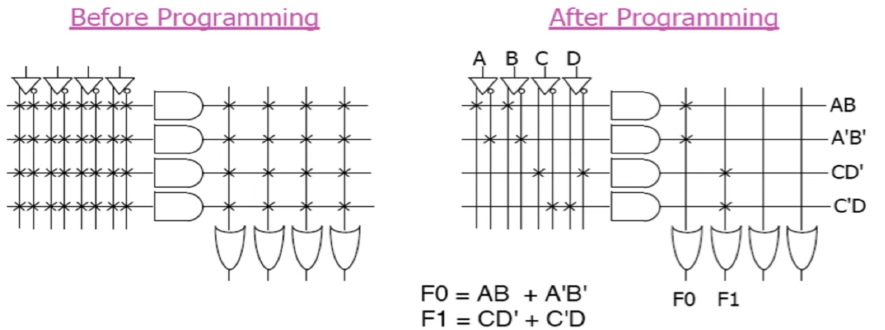
\includegraphics[width=0.86\linewidth]{bf.png}
\end{center}

\noindent\textbf{Esempio}: con 4 ingressi $A,B,C,D$ e 4 implicanti programmati
($AB$,~$A'B'$,~$CD'$,~$C'D$) si implementano le due funzioni:
\[
F_0 = AB + A'B' \qquad\quad F_1 = CD' + C'D = C \oplus D
\]

\defbox{
La \textbf{PLA} risparmia area rispetto alla ROM perché genera \emph{solo} gli implicanti
necessari e non tutti i $2^n$ mintermini. Il numero di righe del piano AND è uguale al
numero di implicanti distinti scelti (non a $2^n$).
}

% ======================================================================
\section{Multiplexer e demultiplexer}

\defbox{
\textbf{MUX} (multiplexer) = circuito digitale che funziona similmente a un selettore,
ma con $2^n$ ingressi, $n$ linee di controllo e 1 uscita.
}

\begin{fitcenter}
\begin{tikzpicture}[scale=0.88, every node/.style={scale=0.88}]
%--- MUX generico ---
\draw (0,0) rectangle (1.8,3.0);
\node at (0.9,1.5) {$2^n$};
% ingressi dati
\foreach \y in {2.5,2.0,1.0,0.5}{
  \draw[-latex] (-1.0,\y) -- (0,\y);
}
\node[left] at (-1.1,1.5) {ingressi};
\node[left,font=\scriptsize] at (-1.1,0.7) {$\vdots$};
% linee di controllo
\draw[-latex] (0.9,-0.8) -- (0.9,0) node[near start,right,font=\scriptsize]{$n$ linee di controllo};
% uscita
\draw[-latex] (1.8,1.5) -- (2.8,1.5) node[right]{uscita};

%--- Freccia =>  ---
\node at (4.2,1.5) {$\Rightarrow$};

%--- MUX 2:1 (con n=1) ---
\begin{scope}[xshift=5.0cm]
% corpo trapezoidale
\draw (0,0.3) -- (1.6,0.8) -- (1.6,2.2) -- (0,2.7) -- cycle;
\node[font=\scriptsize] at (0.75,1.5) {MUX};
% ingressi a0, a1
\draw[-latex] (-0.9,2.3) -- (0,2.3) node[midway,above,font=\scriptsize]{$a_0$};
\draw[-latex] (-0.9,0.7) -- (0,0.7) node[midway,above,font=\scriptsize]{$a_1$};
% selettore S
\draw[-latex] (0.75,-0.3) -- (0.75,0.3) node[near start,right,font=\scriptsize]{$S$};
% uscita
\draw[-latex] (1.6,1.5) -- (2.4,1.5) node[right,font=\scriptsize]{uscita};
\node[below=0.1cm,font=\scriptsize] at (0.75,-0.7) {con $n=1$};
\end{scope}

%--- Notazione ---
\begin{scope}[xshift=9.8cm]
\node[font=\small,align=center] at (0,1.8) {si chiama multiplexer};
\node[font=\small] at (0,1.3) {$2^n : m$};
\node[font=\scriptsize,color=noteteal] at (0.9,1.6) {$\leftarrow$ uscite};
\node[font=\scriptsize,color=noteteal] at (0.9,1.0) {$\leftarrow$ ingressi};
\end{scope}
\end{tikzpicture}
\end{fitcenter}

\medskip
\noindent\textbf{Ogni funzione a $n$ variabili può essere implementata con un
multiplexer $2^{n-1}:1$.}

\medskip
\noindent Consideriamo $F(a,b,c)=a\overline{b}+abc$ e costruiamo la
\textbf{tabella di verità funzionale} usando $a$ e $b$ come indirizzi del MUX\,4:1
($2^2=4$ ingressi) e $c$ come eventuale ingresso dati:

\begin{center}
\begin{minipage}{0.30\linewidth}
\begin{tabular}{cc|c}
\toprule
$a$ & $b$ & $D_i$ (MUX input)\\
\midrule
0 & 0 & 0\\
0 & 1 & 0\\
1 & 0 & 1\\
1 & 1 & $c$\\
\bottomrule
\end{tabular}
\end{minipage}%
\hspace{1.2cm}%
\begin{minipage}{0.45\linewidth}
\begin{tikzpicture}[scale=0.82, every node/.style={scale=0.82}]
% MUX 4:1 che implementa F(abc)
\draw (0,0) rectangle (1.8,3.4);
\node[font=\scriptsize] at (0.9,3.0) {MUX 4:1};
% ingressi dati
\draw[-latex] (-1.4,2.8) -- (0,2.8) node[midway,above,font=\tiny]{$D_{00}=0$};
\draw[-latex] (-1.4,2.1) -- (0,2.1) node[midway,above,font=\tiny]{$D_{01}=0$};
\draw[-latex] (-1.4,1.3) -- (0,1.3) node[midway,above,font=\tiny]{$D_{10}=1$};
\draw[-latex] (-1.4,0.6) -- (0,0.6) node[midway,above,font=\tiny]{$D_{11}=c$};
% selettori
\draw[-latex] (0.55,-0.5) -- (0.55,0) node[near start,left,font=\tiny]{$a$};
\draw[-latex] (1.25,-0.5) -- (1.25,0) node[near start,right,font=\tiny]{$b$};
% uscita
\draw[-latex] (1.8,1.7) -- (2.6,1.7) node[right,font=\tiny]{$F$};
\end{tikzpicture}
\end{minipage}
\end{center}

\medskip

\defbox{
\textbf{DEMUX} (demultiplexer) = circuito digitale opposto al MUX, con 1 ingresso,
$n$ linee di controllo e $2^n$ uscite.
}

\begin{fitcenter}
\begin{tikzpicture}[scale=0.88, every node/.style={scale=0.88}]
%--- DEMUX generico ---
\draw (0,0) rectangle (1.8,3.0);
\node at (0.9,1.5) {$2^n$};
% ingresso
\draw[-latex] (-1.0,1.5) -- (0,1.5) node[midway,above,font=\scriptsize]{ingresso $I$};
% linee di controllo
\draw[-latex] (0.9,-0.8) -- (0.9,0) node[near start,right,font=\scriptsize]{$n$ linee di controllo};
% uscite
\foreach \y in {2.5,2.0,1.0,0.5}{
  \draw[-latex] (1.8,\y) -- (2.8,\y);
}
\node[right,font=\scriptsize] at (2.9,1.5) {$2^n$ uscite};

%--- Freccia ---
\node at (4.4,1.5) {$\Rightarrow$};

%--- DEMUX 1:2 (con n=1) ---
\begin{scope}[xshift=5.2cm]
\draw (0,0.8) -- (0,2.2) -- (1.6,2.7) -- (1.6,0.3) -- cycle;
\node[font=\scriptsize] at (0.75,1.5) {DEMUX};
% ingresso
\draw[-latex] (-0.9,1.5) -- (0,1.5) node[midway,above,font=\scriptsize]{$D$};
% selettore
\draw[-latex] (0.75,-0.3) -- (0.75,0.8) node[near start,right,font=\scriptsize]{$S$};
% uscite
\draw[-latex] (1.6,2.3) -- (2.4,2.3) node[right,font=\scriptsize]{$o_1$};
\draw[-latex] (1.6,0.7) -- (2.4,0.7) node[right,font=\scriptsize]{$o_0$};
\node[below=0.1cm,font=\scriptsize] at (0.75,-0.7) {con $n=1$};
\end{scope}

%--- Notazione ---
\begin{scope}[xshift=10.0cm]
\node[font=\small,align=center] at (0,1.8) {si chiama multiplexer};
\node[font=\small] at (0,1.3) {$m : 2^n$};
\node[font=\scriptsize,color=noteteal] at (0.9,1.6) {$\leftarrow$ uscite};
\node[font=\scriptsize,color=noteteal] at (0.9,1.0) {$\leftarrow$ ingressi};
\end{scope}
\end{tikzpicture}
\end{fitcenter}

% ======================================================================
\section{Universal Shift Register (USR)}

\defbox{
\textbf{USR} (Universal Shift Register) = dispositivo che permette di mettere dati
in parallelo o in serie e di spostarli a destra e sinistra.
}

\begin{center}
\begin{tikzpicture}[scale=0.88, every node/.style={scale=0.88}]
% Tre celle n-1, n, n+1
\foreach \xi/\lab in {0/$n{-}1$, 2.8/$n$, 5.6/$n{+}1$}{
  \draw (\xi,0) rectangle (\xi+2.2,1.6);
  \node at (\xi+1.1,0.8) {\lab};
}
% Frecce rosse shift left (da destra a sinistra)
\draw[-latex,red,thick] (2.8,1.2) -- (2.2,1.2);
\draw[-latex,red,thick] (5.6,1.2) -- (5.0,1.2);
\draw[-latex,red,thick] (-0.7,1.2) -- (0,1.2);
\draw[-latex,red,thick] (7.8,1.2) -- (7.2,1.2) node[right,black,font=\scriptsize]{$\leftarrow$ shift left};
% Frecce blu/verde shift right (da sinistra a destra)
\draw[-latex,teal,thick] (2.2,0.4) -- (2.8,0.4);
\draw[-latex,teal,thick] (5.0,0.4) -- (5.6,0.4);
\draw[-latex,teal,thick] (-0.7,0.4) -- (0,0.4) node[right,black,font=\scriptsize]{};
\draw[-latex,teal,thick] (7.2,0.4) -- (7.9,0.4) node[right,black,font=\scriptsize]{shift right $\rightarrow$};
% Frecce verdi parallelo (dall'alto)
\foreach \xi in {1.1,3.9,6.7}{
  \draw[-latex,green!60!black,thick] (\xi,2.2) -- (\xi,1.6);
}
\node[above,font=\scriptsize,color=green!50!black] at (3.9,2.2) {caricamento parallelo};
% S0, S1
\draw[-latex] (-0.7,-0.5) -- (-0.7,0) node[below=0.4cm,font=\scriptsize]{$S_0$};
\draw[-latex] (0.0,-0.5) -- (0.0,0)  node[below=0.4cm,font=\scriptsize]{$S_1$};
\end{tikzpicture}
\end{center}

\noindent\textbf{Vediamo come implementare ogni singola unità dell'USR.}

\medskip
\noindent Possiamo guidare le quattro funzioni con un \textbf{MUX 4:1} (2 indirizzi):
HOLD, SHIFT LEFT, SHIFT RIGHT, DATA IN.

\begin{center}
\begin{minipage}{0.28\linewidth}
\begin{tabular}{cc|l}
\toprule
$S_1$ & $S_0$ & Funzione\\
\midrule
0 & 0 & hold\\
0 & 1 & shift right\\
1 & 0 & shift left\\
1 & 1 & data in\\
\bottomrule
\end{tabular}
\end{minipage}%
\hspace{0.8cm}%
\begin{minipage}{0.58\linewidth}
\begin{tikzpicture}[scale=0.85, every node/.style={scale=0.85}]
%--- MUX 4:1 ---
\draw (1.5,0) rectangle (3.0,4.0);
\node[font=\scriptsize\bfseries] at (2.25,3.6) {M};
\node[font=\scriptsize\bfseries] at (2.25,3.2) {U};
\node[font=\scriptsize\bfseries] at (2.25,2.8) {X};
% ingressi dati
\draw[-latex] (0,3.5) -- (1.5,3.5) node[midway,above,font=\tiny]{$Q_n$\;\;(00)};
\draw[-latex] (0,2.5) -- (1.5,2.5) node[midway,above,font=\tiny]{$Q_{n-1}$\;(10)};
\draw[-latex] (0,1.5) -- (1.5,1.5) node[midway,above,font=\tiny]{$Q_{n+1}$\;(01)};
\draw[-latex] (0,0.5) -- (1.5,0.5) node[midway,above,font=\tiny]{$I_n$\;\;\;(11)};
% selettori
\draw[-latex] (1.9,-0.6) -- (1.9,0) node[near start,left,font=\tiny]{$S_1$};
\draw[-latex] (2.6,-0.6) -- (2.6,0) node[near start,right,font=\tiny]{$S_0$};
%--- uscita MUX -> DFF ---
\draw[-latex] (3.0,2.0) -- (4.0,2.0) node[midway,above,font=\tiny]{$D_n$};
%--- DFF ---
\draw (4.0,1.2) rectangle (5.8,2.8);
\node[font=\scriptsize] at (4.9,2.4) {$D$\quad$Q_n$};
% triangolo clock
\draw (4.0,1.5) -- (4.3,1.7) -- (4.0,1.9);
\draw[-latex] (4.9,0.5) -- (4.9,1.2) node[near start,right,font=\tiny]{CLK};
% CLR
\draw[-latex] (4.3,0.5) -- (4.3,1.2) node[near start,left,font=\tiny]{CLR};
% uscita Q_n
\draw[-latex] (5.8,2.0) -- (6.6,2.0) node[right,font=\scriptsize]{$Q_n$};
% feedback Q_n -> input 00
\draw (6.3,2.0) -- (6.3,4.8) -- (-0.4,4.8) -- (-0.4,3.5) -- (0,3.5);
\node[right,font=\tiny,color=noteteal] at (6.6,2.5) {$=$ USR};
\end{tikzpicture}
\end{minipage}
\end{center}

\noindent\textit{Se CLR = 1 si effettua un RESET a 0 sincrono.}

% ======================================================================
\subsection{Implementazione a 4 bit per trasmissione PISO}

\begin{fitcenter}
\begin{tikzpicture}[scale=0.8, every node/.style={scale=0.8}]
% 4 celle USR in cascata
\foreach \i/\xi/\lin in {0/0/$I_0$, 1/2.6/$I_1$, 2/5.2/$I_2$, 3/7.8/$I_3$}{
  \draw (\xi,0.4) rectangle (\xi+2.2,2.4);
  \node[font=\scriptsize] at (\xi+1.1,1.4) {$Q_{\i}$};
  % Ingresso parallelo dall'alto
  \draw[-latex] (\xi+1.1,3.0) -- (\xi+1.1,2.4) node[above=0.5cm,font=\tiny]{\lin};
  % S0 S1 dal basso
  \draw[-latex] (\xi+0.6,-0.3) -- (\xi+0.6,0.4) node[below=0.3cm,font=\tiny]{$S_0$};
  \draw[-latex] (\xi+1.5,-0.3) -- (\xi+1.5,0.4) node[below=0.3cm,font=\tiny]{$S_1$};
}
% collegamento in cascata: Q_i uscita -> Q_{i+1} ingresso seriale
\draw[-latex] (2.2,1.4) -- (2.6,1.4);
\draw[-latex] (4.8,1.4) -- (5.2,1.4);
\draw[-latex] (7.4,1.4) -- (7.8,1.4);
% input sinistro LI (=LSI)
\draw[-latex] (-0.9,1.8) -- (0,1.8) node[midway,above,font=\tiny]{$L_I$};
% input destro RI (=RSI)
\draw[-latex] (10.9,1.0) -- (10.0,1.0) node[midway,above,font=\tiny]{$R_I$};
% uscita sinistra L0
\draw[-latex] (0,1.0) -- (-0.9,1.0) node[left,font=\tiny]{$L_0$};
% uscita destra R0
\draw[-latex] (10.0,1.8) -- (10.9,1.8) node[right,font=\tiny]{$R_0$};
% CLK comune
\draw[-latex] (-1.2,-1.0) -- (-1.2,-1.4) -- (9.8,-1.4);
\foreach \xi in {1.1,3.7,6.3,8.9}{
  \draw[-latex] (\xi,-1.4) -- (\xi,0.4);
}
\node[left,font=\tiny] at (-1.2,-1.0) {CLK};
% CLR comune
\draw[-latex] (-0.6,-0.9) -- (-0.6,-1.9) -- (9.7,-1.9);
\foreach \xi in {0.8,3.4,6.0,8.6}{
  \draw (\xi,-1.9) -- (\xi,-0.3);
  \draw[-latex] (\xi,-0.3) -- (\xi,0.4);
}
\node[left,font=\tiny] at (-0.6,-0.9) {CLR};
% Legenda
\node[align=left,font=\tiny] at (10.5,-0.4) {$L_I = \text{LSI}$\\$R_I = \text{RSI}$\\$L_0 = \text{LSD}$\\$R_0 = \text{RSO}$};
\end{tikzpicture}
\end{fitcenter}

\noindent Il circuito permette 4 modalità operative selezionate da $S_1 S_0$:
caricamento parallelo, shift left (seriale verso sinistra), shift right (seriale verso
destra) e hold.

\subsection{Applicazione: trasmissione seriale Sender--Receiver}

\begin{center}
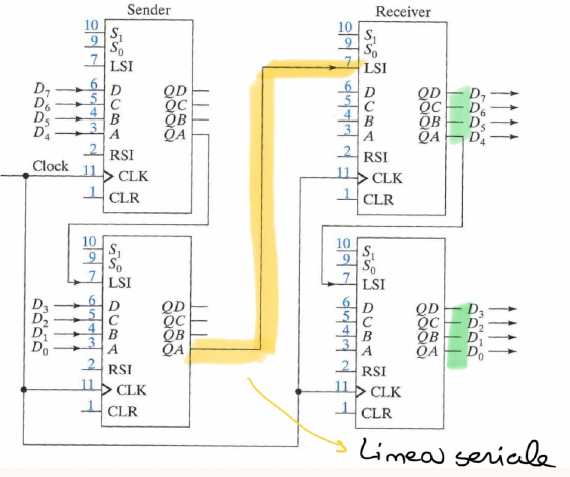
\includegraphics[width=0.78\linewidth]{crl.png}
\end{center}

\noindent Il flusso dell'operazione è:
\[
\text{Caricamento nel Sender di }D_i
\;\xrightarrow{\text{shift}}\;
\text{Trasmissione sulla linea seriale}
\;\xrightarrow{\text{shift}}\;
\text{Lettura sulle uscite del Receiver}
\]

% ======================================================================
\section{Vincoli temporali dell'USR e Jitter}

\noindent La \textbf{massima frequenza del clock} per un USR corrisponde al
\textbf{minimo periodo del clock}:

\[
\boxed{T_{\text{CLK,min}} = T_{\text{setup}} + T_{\text{propag}} + T_{\text{lc}} + T_{\text{jitter}}}
\]

\begin{center}
\begin{tikzpicture}[scale=0.9, every node/.style={scale=0.9}]
% Linea temporale con le 4 componenti
\draw[-latex] (0,0) -- (9.5,0) node[right]{$t$};
% Segmenti
\draw[thick,teal]   (0,0)   -- (2.0,0);
\draw[thick,orange] (2.0,0) -- (4.2,0);
\draw[thick,blue]   (4.2,0) -- (6.5,0);
\draw[thick,red]    (6.5,0) -- (8.5,0);
% tick marks
\foreach \x in {0,2.0,4.2,6.5,8.5}{
  \draw (\x,0.15) -- (\x,-0.15);
}
% etichette
\node[above,font=\scriptsize,color=teal]   at (1.0,0.1) {$T_{\text{propag}}$};
\node[above,font=\scriptsize,color=orange] at (3.1,0.1) {$T_{\text{lc}}$};
\node[above,font=\scriptsize,color=blue]   at (5.35,0.1) {$T_{\text{setup}}$};
\node[above,font=\scriptsize,color=red]    at (7.5,0.1) {$T_{\text{jitter}}$};
% frecce-descrizione
\node[below,font=\tiny,color=teal,align=center]   at (1.0,-0.3) {ritardo\\CLK$\to Q$ nel FF};
\node[below,font=\tiny,color=orange,align=center] at (3.1,-0.3) {ritardo logica\\comb.\ (MUX)};
\node[below,font=\tiny,color=blue,align=center]   at (5.35,-0.3) {stabilità per\\CLK successivo};
\node[below,font=\tiny,color=red,align=center]    at (7.5,-0.3) {jitter del CLK};
\end{tikzpicture}
\end{center}

\defbox{
\textbf{Jitter del CLK} = $\Delta_{\max}$ fra gli istanti di arrivo dei fronti di clock
che dovrebbero giungere \emph{contemporaneamente} a tutti i componenti del circuito, ma
che in pratica non lo fanno a causa di variazioni fisiche (disadattamenti di linea,
rumore, disomogeneità dei percorsi).
}


% ======================================================================
\chapter{Conversione Digitale--Analogica e Analogica--Digitale}
\textit{(15 maggio 2026)}

% ======================================================================
\section{Conversione digitale $\leftrightarrow$ analogica}

Il processo di acquisizione e ricostruzione del segnale si articola in due fasi:

\begin{center}
\begin{tikzpicture}[scale=0.85, every node/.style={scale=0.85},
  box/.style={draw, minimum width=1.6cm, minimum height=0.8cm, align=center, font=\small},
  arr/.style={-latex,thick}]

% --- segnale analogico campionato ---
\node[font=\small] at (0,2.2) {$\Delta V$};
\draw[arr] (-0.2,0) -- (4.2,0); \node[right,font=\scriptsize] at (4.2,0) {$t$};
\draw[arr] (0,-0.2) -- (0,2.0);
\foreach \x/\h in {0.5/1.2, 1.0/1.6, 1.5/1.8, 2.0/1.5, 2.5/1.0, 3.0/0.8, 3.5/1.3}{
  \draw[blue,thick] (\x,0) -- (\x,\h);
  \fill[blue] (\x,\h) circle (2pt);
}
\node[above,font=\scriptsize] at (2.0,2.2) {campionamenti $V(t_i)$};

% --- blocchi Sensore -> ADC ---
\node[box] (sens) at (5.8,0.9) {Sensore};
\node[box] (adc)  at (7.8,0.9) {ADC};
\draw[arr] (4.5,0.9) -- (sens.west);
\draw[arr] (sens.east) -- (adc.west);
\draw[arr] (adc.south) -- ++(0,-0.5) node[below,font=\scriptsize,align=center]{convertitore\\analogico$\to$digitale};
\draw[arr] (adc.east)  -- ++(1.0,0);

% --- segnale ricostruito ---
\begin{scope}[xshift=9.5cm]
\node[font=\small] at (0,2.2) {$\Delta V$};
\draw[arr] (-0.2,0) -- (4.2,0); \node[right,font=\scriptsize] at (4.2,0) {$t$};
\draw[arr] (0,-0.2) -- (0,2.0);
\foreach \x/\h in {0.5/1.2, 1.0/1.6, 1.5/1.8, 2.0/1.5, 2.5/1.0, 3.0/0.8, 3.5/1.3}{
  \fill[blue] (\x,\h) circle (2pt);
}
\draw[blue,thick,domain=0.5:3.5,samples=60] plot(\x,{1.5+0.4*sin(3.14159*\x r)+0.3*cos(6.28*\x r)});
\node[above,font=\scriptsize] at (2.0,2.3) {estrapolazioni lineari};
\node[below,font=\scriptsize] at (2.0,-0.3) {dopo l'elaborazione del segnale};
\end{scope}
\end{tikzpicture}
\end{center}

\noindent Il quesito è: cosa succede fra il campionamento e la ricostruzione? La risposta è
\textbf{sample and hold} $\to$ \textbf{convertitore analogico$\to$digitale} $\to$ \textbf{convertitore digitale$\to$analogico}, in sintesi:
\[
\text{Sensore} \;\xrightarrow{\text{ADC}}\; \text{elaborazione digitale} \;\xrightarrow{\text{DAC}}\; \text{uscita analogica}
\]

\noindent Definizioni di base:
\begin{itemize}[leftmargin=1.5em]
    \item $n_{(\cdot)}$ = numero che dipende dai bit disponibili;
    \item $\Delta V$ = \textbf{granularità}, ovvero il passo minimo distinguibile;
    \item $V_{\text{ref}}$ = valore massimo attingibile.
\end{itemize}

\defbox{
\textbf{Funzione di trasferimento di un ADC}: $\quad n_{\text{out}} = V_{\text{in}}/\Delta V$\\[0.3em]
\textbf{Funzione di trasferimento di un DAC}: $\quad V_{\text{out}} = n_{\text{in}} \cdot \Delta V$
}

% ======================================================================
\section{Caratteristiche del DAC}

\defbox{
\textbf{Precisione} = determinata dal numero di bit e dall'intervallo di tensioni:
\[
V_{\text{out}} = n_{\text{in}} \cdot \Delta V
\]
Ad esempio, con $n$-bit $= 3$ e $\Delta V = 1\,\text{V}$:
$n_{\text{in}} \in [0,\, 2^3{-}1] \;\Rightarrow\; V_{\text{out}} \in [0,\, 2^3{-}1]\,\text{V}$.
}

\noindent La velocità di conversione è molto importante e dipende da diversi fattori: tipo di
assestamento, architettura e numero di bit. Le tre principali sorgenti di errore nel DAC sono:

\begin{center}
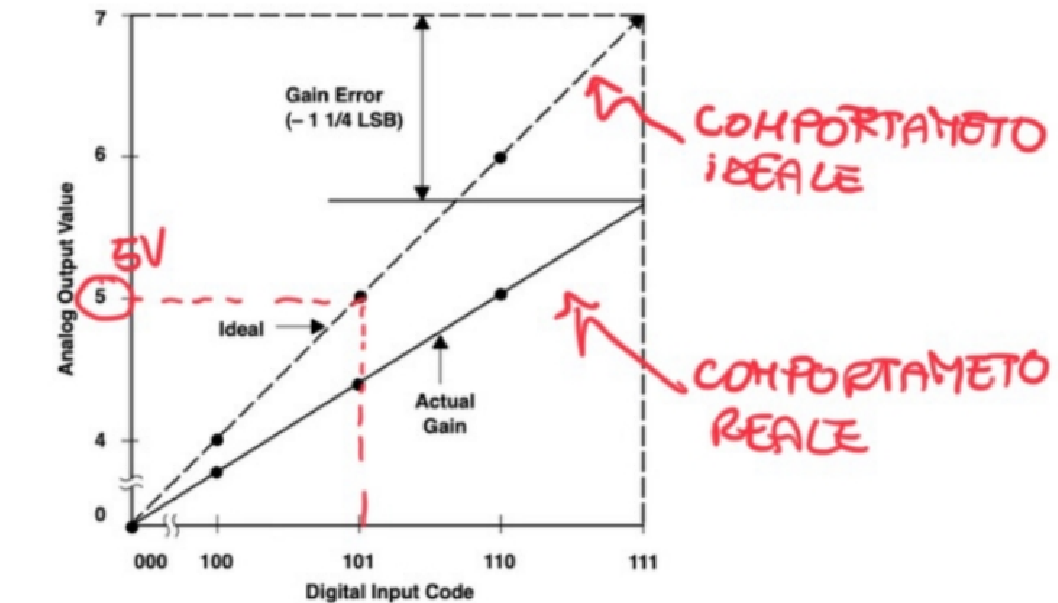
\includegraphics[width=0.32\linewidth]{err_g.png}\hfill
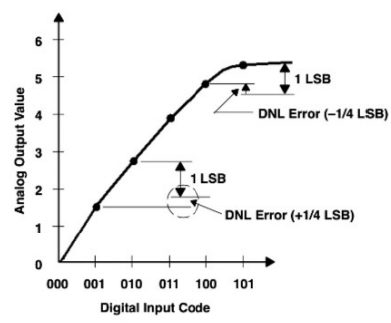
\includegraphics[width=0.32\linewidth]{n_lin.png}\hfill
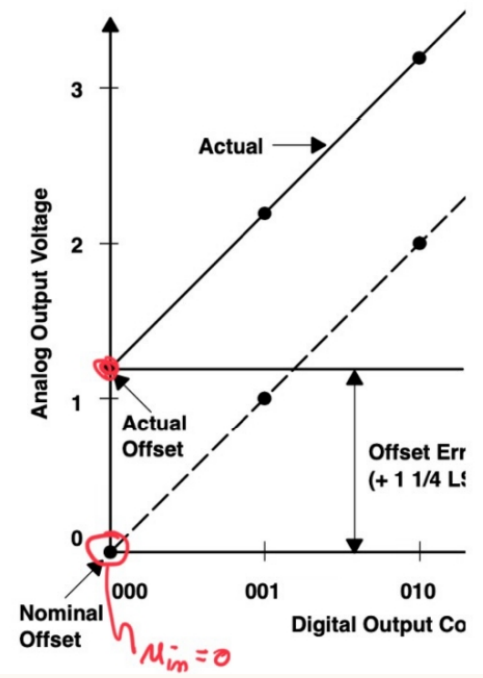
\includegraphics[width=0.32\linewidth]{er_nlin.png}
\end{center}

% ======================================================================
\section{DAC a sommatore}

L'architettura più semplice di DAC è il \textbf{DAC a sommatore pesato}: si usa un
amplificatore operazionale invertente con resistenze pesate $R_i = R/2^i$ per ciascun
bit. Le resistenze di ingresso sono collegate a $V_{\text{ref}}$ (bit $a_i=1$) o a massa
(bit $a_i=0$) tramite uno switch digitale per ciascun bit.

\begin{center}
\begin{circuitikz}[scale=0.85, every node/.style={scale=0.85}, american voltages]

\node[op amp, noinv input up] (OA) at (4.0,0) {};

% Resistenza di retroazione R
\draw (OA.out) -- ++(0,1.4) to[R, l=$R$] ++(-2.4,0) -- ++(0,-0.55);

% Nodo sommatore (ingresso invertente)
\draw (OA.-) -- ++(-0.4,0) coordinate (suma);

% Bit a0 (MSB)
\draw (suma) -- ++(0,+0.9) to[R, l=$R$, -*] ++(-1.8,0)
      node[left]{$V_{\text{ref}}$} node[above right,font=\scriptsize]{$a_0$ (MSB)};

% Bit a1
\draw (suma) to[R, l=$2R$, -*] ++(-1.8,0)
      node[left]{$V_{\text{ref}}$} node[above right,font=\scriptsize]{$a_1$};

% Bit a2 (LSB)
\draw (suma) -- ++(0,-0.9) to[R, l=$4R$, -*] ++(-1.8,0)
      node[left]{$V_{\text{ref}}$} node[above right,font=\scriptsize]{$a_2$ (LSB)};

% Massa sul + dell'OA
\draw (OA.+) -- ++(0,-0.4) node[ground]{};

% Uscita
\draw (OA.out) -- ++(0.8,0) node[right]{$V_{\text{out}}$};

\end{circuitikz}
\end{center}

\noindent\textit{Nota}: ogni ramo $a_i$ è collegato a $V_{\text{ref}}$ tramite uno switch
digitale, che si chiude o si apre (collegando in alternativa a massa) a seconda del valore
del bit; il simbolo del cursore $\updownarrow$ negli appunti originali indica proprio questo
switch a monte dell'ingresso invertente.

\noindent La formula di uscita si ricava dalla sovrapposizione degli effetti:
\[
V_{\text{out}} = -V_{\text{ref}}\!\left(\frac{R}{R_0}+\frac{R}{R_1}+\frac{R}{R_2}\right)
\]
Se si pone $R_i = R/2^i$, allora $R/R_i = 2^i$ e quindi:
\[
\boxed{V_{\text{out}} = -V_{\text{ref}}\sum_i 2^i}
\]
Considerando gli switch digitali, ogni bit $a_i$ vale 0 (collegamento a terra) oppure 1
(collegamento a $V_{\text{ref}}$):
\[
\boxed{V_{\text{out}} = -V_{\text{ref}}\sum_i a_i\,2^i}
\]

\medskip
\noindent\textbf{Limite pratico}: supponendo 10 bit, $R_i = 100\,\text{k}\Omega/2^i$.
Se la tolleranza è $\sigma_0 = 1\%$ e $R_0 = 1\,\text{k}\Omega$, i bit meno significativi
vengono persi perché il loro valore di resistenza scende sotto la tolleranza stessa
($R_i < \sigma_0$). Questo DAC è quindi utilizzabile solo con pochi bit; altrimenti non è
sufficientemente preciso.

% ======================================================================
\section{DAC R-2R Ladder}

Per avere un DAC più preciso si usa la tecnica \textbf{R-2R Ladder}, che genera pesi
binari per i bit usando solo due valori di resistenza ($R$ e $2R$):

\begin{center}
\begin{circuitikz}[scale=0.85, every node/.style={scale=0.85}, american voltages]

\coordinate (n0) at (0,6.0);   % MSB (bit 0)
\coordinate (n1) at (0,4.0);   % bit 1
\coordinate (n2) at (0,2.0);   % bit 2
\coordinate (n3) at (0,0.0);   % LSB (bit 3)

% Rami 2R orizzontali verso Vref/switch
\foreach \y/\lab in {6.0/0, 4.0/1, 2.0/2, 0.0/3}{
  \draw (0,\y) to[R, l=$2R$] (-2.4,\y);
  \draw[-latex] (-2.4,\y) -- (-3.2,\y) node[left,font=\scriptsize]{$a_{\lab}$};
}

% Rami R verticali tra i nodi
\draw (0,6.0) to[R, l=$R$] (0,4.0);
\draw (0,4.0) to[R, l=$R$] (0,2.0);
\draw (0,2.0) to[R, l=$R$] (0,0.0);

% Terminazione a massa
\draw (0,0.0) to[R, l=$R$] (0,-1.6) node[ground]{};

% Linea di uscita verso OA
\draw (0,6.0) -- (1.0,6.0) coordinate (vout_line);

% OpAmp
\node[op amp, noinv input up] (OA) at (3.5,5.2) {};
\draw (vout_line) -- (OA.-);
\draw (OA.+) -- ++(0,-0.4) node[ground]{};
\draw (OA.out) -- ++(0,1.2) to[R, l=$2R$] ++(-2.6,0) -- ++(0,-0.6);
\draw (OA.out) -- ++(0.8,0) node[right]{$V_{\text{out}}$};

\node[right,font=\scriptsize,color=noteblue] at (0.2,6.0) {MSB};
\node[right,font=\scriptsize,color=noteblue] at (0.2,0.0) {LSB};

\end{circuitikz}
\end{center}

\noindent Ogni bit $a_i$ contribuisce all'uscita con un peso binario:
\[
a_i \;\longrightarrow\; V_{\text{out},i} = -\frac{V_{\text{ref}}}{2^{i+1}}
\qquad\Rightarrow\quad
\text{i pesi sono } \frac{1}{2},\,\frac{1}{4},\,\frac{1}{8},\,\frac{1}{16},\ldots
\]
\[
\boxed{V_{\text{out}} = -V_{\text{ref}}\sum_i \frac{a_i}{2^{i+1}}}
\]

\noindent\textbf{Esempio}: con 4 bit, ingresso $1010_2$ e $V_{\text{ref}} = 8\,\text{V}$:
\[
V_{\text{out}} = -8\!\left(\frac{1}{2}+\frac{1}{8}\right) = -8 \cdot \frac{5}{8} = -5\,\text{V}
\]

% ======================================================================
\section{Caratteristiche dell'ADC}

\begin{itemize}[leftmargin=1.5em]
    \item \textbf{Accuratezza} = insieme di tutte le sorgenti di errore, errore di
          quantizzazione compreso.
    \item \textbf{Errore di quantizzazione} = dipende dal tipo di ADC ed è dovuto alla
          discretizzazione del segnale durante la conversione; di solito vale $1$ LSB
          oppure $0{,}5$ LSB.
    \item \textbf{Tempo di conversione} e \textbf{funzionamento} sono altre caratteristiche
          importanti dell'ADC.
\end{itemize}

\noindent Analogamente al DAC, anche l'ADC presenta tre principali tipi di errore rispetto
al comportamento ideale:

\begin{center}
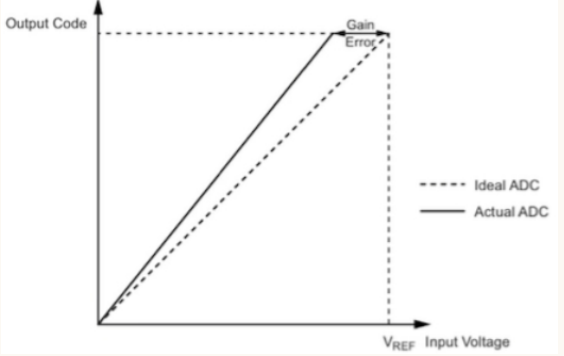
\includegraphics[width=0.32\linewidth]{err_g2.png}\hfill
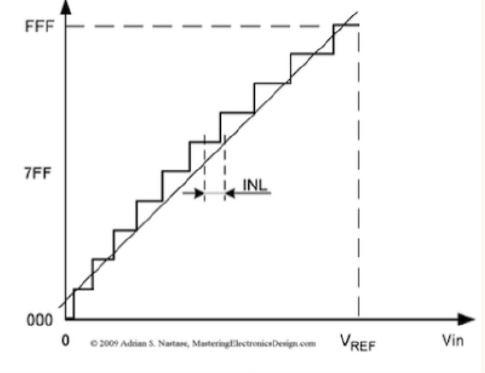
\includegraphics[width=0.32\linewidth]{n_lin2.png}\hfill
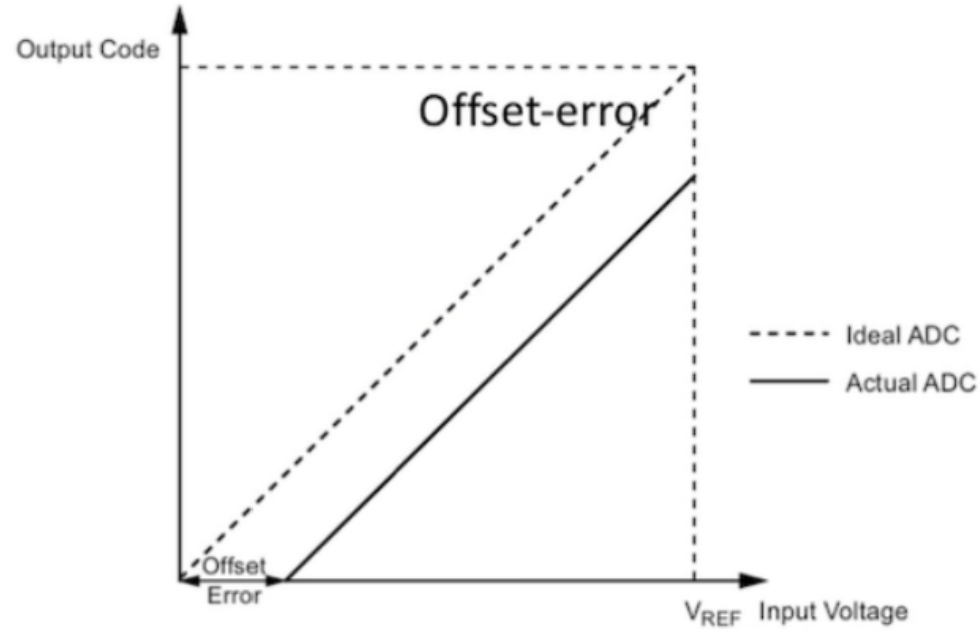
\includegraphics[width=0.32\linewidth]{er_nlin2.png}
\end{center}

% ======================================================================
\chapter{Convertitori Analogico-Digitali (ADC)}
\textit{(15 maggio 2026 -- cont.)}

% ---------- BLOCCO 1: ADC a gradinata ----------
\section{ADC a gradinata}

\noindent
\begin{minipage}[t]{0.42\textwidth}
    \vspace{0pt}
    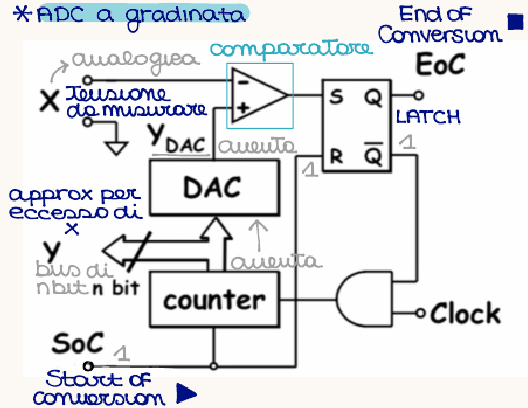
\includegraphics[width=\textwidth]{11.png}
\end{minipage}%
\hfill
\begin{minipage}[t]{0.55\textwidth}
    \vspace{0pt}
    \begin{itemize}[leftmargin=1em]
        \item \textbf{Funzionamento del comparatore}: finché $X > Y_{DAC}$ il conteggio procede; appena $Y_{DAC} \geq X$ il comparatore cambia stato $\rightarrow$ il latch RS blocca il \texttt{CLK} e il \texttt{counter}.
        \item \textbf{Funzionamento del contatore}: genera $N_{in_2} \rightarrow N_{in_0}$ e aumenta la tensione.
        \item La granularità dipende da $V_{REF}$ del DAC (cioè il $\Delta V$ con cui aumenta).
        \item Asintoticamente questo ADC deve fare $2^{n}$ confronti, dove $n$ sono i livelli del DAC:
        \begin{equation*}
            T_{conv} = 2^{n} \, T_{CLK}
        \end{equation*}
    \end{itemize}
\end{minipage}

\vspace{1.5em}

% ---------- BLOCCO 2: ADC SAR ----------
\section{ADC ad approssimazioni successive (SAR)}

\noindent
\begin{minipage}[t]{0.42\textwidth}
    \vspace{0pt}
    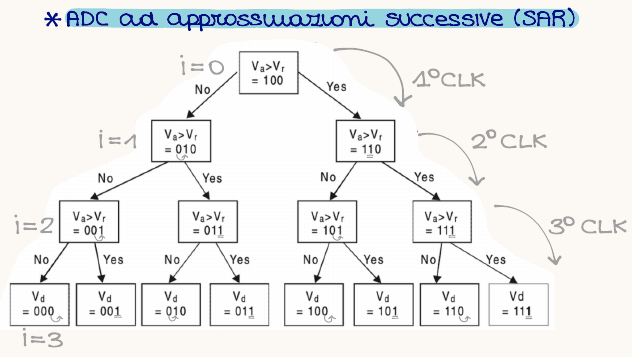
\includegraphics[width=\textwidth]{22.png}
\end{minipage}%
\hfill
\begin{minipage}[t]{0.55\textwidth}
    \vspace{0pt}
    \begin{itemize}[leftmargin=1em]
        \item Il valore di tensione da misurare si confronta con i successivi.
        \item Ogni conversione avviene in un ciclo di \texttt{CLK}. Se $n_{bit}=3$ ci sono 3 cicli.
        \item \textbf{Yes}: metto un 1 nella posizione $i+1$ se passo da $i$ a $i+1$.
        \item \textbf{No}: sposto l'1 dalla posizione $i$ alla posizione $i+1$ passando da $i$ a $i+1$.
        \item È una ricerca binaria: i confronti sono $n$, quindi:
        \begin{equation*}
            T_{conv} = n \, T_{CLK}
        \end{equation*}
        \item Funzionamento specifico alla pagina successiva.
    \end{itemize}
\end{minipage}

\vspace{1.5em}

% ---------- BLOCCO 3: FLASH ADC ----------
\section{Flash ADC}

\noindent
\begin{minipage}[t]{0.42\textwidth}
    \vspace{0pt}
    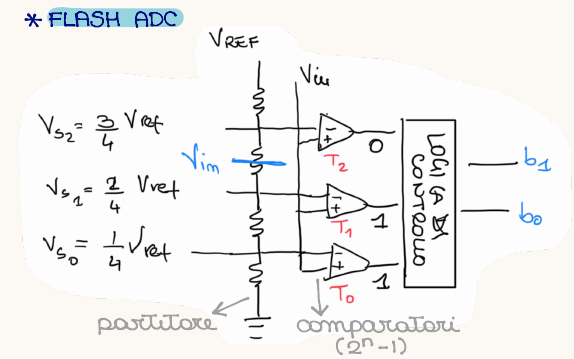
\includegraphics[width=\textwidth]{33.png}
\end{minipage}%
\hfill
\begin{minipage}[t]{0.55\textwidth}
    \vspace{0pt}
    \begin{itemize}[leftmargin=1em]
        \item La tensione viene confrontata contemporaneamente con $n$ valori; poi un circuito combinatorio converte le uscite dei confronti in binario (1 = valori coperti da $V_{in}$; 0 = valori più alti di $V_{in}$).
        \item Un confronto: istantaneo (fatto in parallelo) $\Rightarrow$ è il più veloce.
        \item La precisione è però molto minore di quella degli altri (servono tante resistenze, con i problemi già discussi).
        \item Risolvo coi mintermini, sapendo che se $j < i < k$ e $T_i = 1$ allora $T_j = 1$ e $T_k = 0$:
        \begin{align*}
            b_0 &= T_2 + T_0 \cdot T_1 \\
            b_1 &= T_2 + T_1 \cdot \overline{T_2}
        \end{align*}
    \end{itemize}
\end{minipage}

\vspace{1.5em}

\section{Osservazioni generali}
\begin{itemize}[leftmargin=1.5em]
    \item L'errore di quantizzazione è pari a $0{,}5 \, V_{REF}/2^{n}$.
\end{itemize}

\section{ADC dell'AD2}
\begin{itemize}[leftmargin=1.5em]
    \item Ci sono \SI{14}{bit} $\Rightarrow 2^{14}$ possibili valori.
    \item Se scelgo la scala \SI{0.5}{\volt}/div l'intervallo in cui misuro è $(0, 0{,}5 \cdot 10)\,\si{\volt} = (0,5)\,\si{\volt}$, e la quantizzazione è:
    \begin{equation*}
        \frac{\SI{5}{\volt}}{2^{14}} \approx \SI{0.3}{\milli\volt}
    \end{equation*}
\end{itemize}

% ============================================================
% ADC ad approssimazioni successive (SAR) - Circuito a 3 bit
% Spiegazione dettagliata basata sulle slide
% ============================================================

\subsection{ADC ad approssimazioni successive (SAR): analisi del circuito a 3 bit}

Il convertitore analogico--digitale ad \emph{approssimazioni successive} (in inglese \textbf{S}uccessive \textbf{A}pproximation \textbf{R}egister, SAR) determina il codice digitale corrispondente ad una tensione analogica $V_a$ eseguendo un confronto ``dicotomico'' bit a bit, a partire dal bit più significativo (MSB) fino al meno significativo (LSB). Il circuito visto a lezione realizza un SAR a 3 bit ed è composto dai seguenti blocchi funzionali:

\begin{itemize}
    \item \textbf{Ring Counter} (registro a scorrimento circolare) costituito da 5 flip-flop $S_0,\dots,S_4$: genera, un colpo di clock alla volta, un impulso che si sposta da uno stadio al successivo. Questo impulso scandisce il tempo di test di ciascun bit (MSB $\to$ LSB) e determina quando la conversione è terminata.
    \item \textbf{Registro dei bit di prova} composto da 3 flip-flop $Q_2, Q_1, Q_0$ (MSB $\to$ LSB): contiene, istante per istante, il codice binario di tentativo.
    \item \textbf{DAC} (convertitore digitale--analogico): converte il codice presente in $Q_2Q_1Q_0$ nella tensione di confronto $V_{DAC}$.
    \item \textbf{Comparatore analogico}: confronta $V_a$ (tensione incognita da convertire) con $V_{DAC}$.
    \item \textbf{Logica combinatoria (porte AND/OR)}: in base all'uscita del comparatore e allo stadio attivo del Ring Counter, decide se mantenere a 1 oppure resettare a 0 il bit appena testato.
\end{itemize}

\`E importante notare che il Ring Counter e il registro dei bit di prova lavorano \emph{in parallelo}: mentre il Ring Counter ``punta'' al bit che si sta testando in quel colpo di clock, il registro $Q_2Q_1Q_0$ contiene il codice di prova corrente, che viene aggiornato bit dopo bit.

\bigskip
\subsubsection{Fase 1 -- Inizializzazione (prima del primo fronte di clock)}

Prima dell'arrivo del primo fronte di clock il circuito viene inizializzato nel seguente modo:

\begin{enumerate}
    \item Si invia il segnale di \texttt{CLEAR} (attivo basso) contemporaneamente a tutti i flip-flop del registro dati $Q_2,Q_1,Q_0$: tutte le uscite vengono forzate a 0.
    \item Contemporaneamente si setta $S_0=1$ (primo stadio del Ring Counter) tramite ingresso asincrono, mentre tutti gli altri stadi $S_1,\dots,S_4$ vengono inizializzati a 0.
    \item Poich\'e il registro dati è tutto a 0, l'ingresso del DAC è $000$, quindi l'uscita del DAC è
    \[
        V_{DAC} = 0\ \text{V}.
    \]
\end{enumerate}

Lo stato del sistema subito prima del primo fronte di clock è dunque:
\[
(S_4 S_3 S_2 S_1 S_0) = (0\,0\,0\,0\,1), \qquad (Q_2 Q_1 Q_0) = (0\,0\,0), \qquad V_{DAC}=0\text{ V}.
\]

\bigskip
\subsubsection{Fase 2 -- Subito dopo il primo fronte di clock}

Al primo fronte di clock accadono due cose contemporaneamente:

\begin{itemize}
    \item Il Ring Counter avanza di uno stadio: $S_0 \to 0$, $S_1 \to 1$. Questo impulso su $S_1$ abilita la scrittura del bit più significativo $Q_2$.
    \item La logica combinatoria pone \emph{a priori} $Q_2 = 1$ (si ``prova'' il bit più significativo settandolo a 1): il nuovo codice di prova è $Q_2Q_1Q_0 = 100$.
\end{itemize}

Con il nuovo codice in ingresso, il DAC produce la tensione corrispondente a $n=4$ (in decimale):
\[
V_{DAC} = V(n{=}4) \quad \text{(tensione corrispondente al codice \texttt{100})}.
\]

A questo punto il comparatore confronta $V_a$ con $V_{DAC}$: il risultato di questo confronto sarà disponibile e utilizzato al fronte di clock \emph{successivo} per decidere se mantenere $Q_2=1$ oppure resettarlo a 0.

\bigskip
\subsubsection{Esempio numerico}

Supponiamo che il DAC abbia una risoluzione $\Delta V = 1\text{ V}$ sull'intervallo $[0,7]\text{ V}$ (3 bit, 8 livelli) e che la tensione incognita sia
\[
V_a = 5.5\text{ V}.
\]

Dopo il primo fronte di clock il registro contiene $Q_2Q_1Q_0=100$, quindi
\[
V_{DAC} = 4\text{ V}.
\]

Il comparatore verifica se $V_a > V_{DAC}$ (equivalentemente, se $V_a$ supera la metà del fondo scala, $V_{max}/2$):
\[
V_a = 5.5\text{ V} > V_{DAC}=4\text{ V} \quad\Longrightarrow\quad \text{SI}.
\]

Poich\'e il confronto ha dato esito positivo, il bit $Q_2$ appena testato viene \textbf{mantenuto a 1} (l'approssimazione ``per difetto'' era corretta: la tensione reale è maggiore di quella generata dal DAC con quel bit a 1, quindi quel bit resta valido nel codice finale).

\bigskip
\subsubsection{Fase 4 -- Subito dopo il secondo fronte di clock}

Al secondo fronte di clock:

\begin{itemize}
    \item Il Ring Counter avanza ancora: $S_1\to 0$, $S_2\to 1$. L'impulso su $S_2$ abilita ora la scrittura del bit successivo $Q_1$.
    \item Il risultato del confronto precedente (esito ``SI'', $V_a>V_{DAC}$) viene usato dalla logica combinatoria per \textbf{confermare} $Q_2=1$ definitivamente.
    \item Contemporaneamente si prova il nuovo bit ponendo $Q_1=1$: il codice di prova diventa $Q_2Q_1Q_0 = 110$.
\end{itemize}

Il DAC aggiorna quindi la propria uscita al nuovo codice:
\[
V_{DAC} = 4\text{ V} + 2\text{ V} = 6\text{ V}.
\]

Si esegue un nuovo confronto:
\[
V_a = 5.5\text{ V} < V_{DAC} = 6\text{ V} \quad\Longrightarrow\quad \text{esito negativo}.
\]

Questa volta il bit appena provato ($Q_1$) risulter\`a, al fronte di clock successivo, \textbf{resettato a 0} (il DAC ha superato $V_a$, quindi quel bit non pu\`o essere 1 nel codice finale): il codice torna a $100$ per quanto riguarda $Q_2Q_1$, e si passer\`a a testare l'ultimo bit $Q_0$.

\bigskip
\subsubsection{Algoritmo generale (n bit)}

Il procedimento si generalizza a un ADC-SAR a $n$ bit come segue: per ogni bit, dal MSB al LSB,

\begin{enumerate}
    \item il Ring Counter abilita la scrittura del bit corrente;
    \item la logica pone a 1 (in via di prova) il bit corrente, lasciando invariati i bit gi\`a decisi in precedenza;
    \item il DAC converte il nuovo codice di prova in $V_{DAC}$;
    \item il comparatore confronta $V_a$ con $V_{DAC}$;
    \item al fronte di clock successivo, in base al risultato del confronto:
    \begin{itemize}
        \item se $V_a > V_{DAC}$: il bit resta a 1 (viene confermato);
        \item se $V_a < V_{DAC}$: il bit viene riportato a 0.
    \end{itemize}
\end{enumerate}

Il processo richiede quindi $n$ colpi di clock per determinare i bit, pi\`u un colpo aggiuntivo di inizializzazione/lettura: per questo il Ring Counter dell'esempio ha 5 stadi ($S_0,\dots,S_4$) per un ADC a 3 bit (1 stadio di start + 3 stadi di conversione + 1 stadio di fine conversione/lettura del risultato).

\bigskip
\subsubsection{Tabella riassuntiva dell'esempio ($V_a = 5.5$~V)}

\begin{center}
\begin{tabular}{c c c c c}
\hline
\textbf{Fronte di clock} & \textbf{Bit testato} & \textbf{Codice di prova} $Q_2Q_1Q_0$ & $V_{DAC}$ & \textbf{Confronto} $V_a \gtrless V_{DAC}$ \\
\hline
1 (init.) & $Q_2$ & $100$ & $4$ V & $5.5 > 4 \Rightarrow$ mantieni \\
2          & $Q_1$ & $110$ & $6$ V & $5.5 < 6 \Rightarrow$ resetta \\
3          & $Q_0$ & $101$ & $5$ V & $5.5 > 5 \Rightarrow$ mantieni \\
\hline
\end{tabular}
\end{center}

Il codice digitale finale \`e dunque $Q_2Q_1Q_0 = 101$ (decimale 5), corrispondente a $V_{DAC}=5$~V: il valore pi\`u vicino per difetto a $V_a=5.5$~V ottenibile con una risoluzione di 1~V (errore di quantizzazione $=0.5$~V, cio\`e met\`a del passo, come atteso).

% ============================================================
% ADC SAR a 3 bit - Continuazione: Fasi 5-9
% (da aggiungere subito dopo la sezione "Fase 4" del file precedente)
% ============================================================

\subsubsection{Fase 5 -- Valutazione del confronto (subito dopo il secondo fronte)}

Nello stesso ciclo di clock in cui $Q_1$ è stato posto a 1 (Fase 4), il comparatore valuta il nuovo confronto tra $V_a$ e la $V_{DAC}$ appena aggiornata:
\[
V_a = 5.5\text{ V} \quad \text{vs} \quad V_{DAC} = 6\text{ V}.
\]
Poich\'e
\[
V_a = 5.5\text{ V} < V_{DAC} = 6\text{ V},
\]
l'esito del confronto è \textbf{negativo}: il bit $Q_1$ appena provato \emph{non} sar\`a confermato. Questo risultato viene memorizzato dalla logica combinatoria e sar\`a applicato al registro dati al fronte di clock \emph{successivo} (Fase 6): la fase di ``confronto'' è quindi concettualmente distinta dalla fase di ``scrittura'', anche se entrambe avvengono nello stesso periodo di clock.

\bigskip
\subsubsection{Fase 6 -- Subito dopo il terzo fronte di clock}

Al terzo fronte di clock accadono, come nei casi precedenti, due cose:

\begin{itemize}
    \item Il Ring Counter avanza: $S_2\to 0$, $S_3\to 1$. L'impulso su $S_3$ abilita ora la scrittura del bit meno significativo $Q_0$.
    \item In base al risultato negativo della Fase 5, il bit $Q_1$ viene \textbf{resettato a 0}: il codice torna ad avere $Q_2Q_1 = 10$.
    \item Contemporaneamente si prova il nuovo bit ponendo $Q_0=1$: il codice di prova diventa $Q_2Q_1Q_0 = 101$.
\end{itemize}

Il DAC aggiorna quindi la propria uscita:
\[
V_{DAC} = 4\text{ V} + 0\text{ V} + 1\text{ V} = 5\text{ V}.
\]

\bigskip
\subsubsection{Fase 7 -- Confronto sull'ultimo bit (LSB)}

Si esegue l'ultimo confronto della conversione:
\[
V_a = 5.5\text{ V} > V_{DAC} = 5\text{ V} \quad\Longrightarrow\quad \text{esito \textbf{positivo} (SI)}.
\]

Il bit $Q_0$ appena provato viene quindi \textbf{mantenuto a 1}. A questo punto tutti e tre i bit sono stati testati e il codice binario è stato completamente determinato:
\[
Q_2 Q_1 Q_0 = 1\,0\,1 \quad (= 5 \text{ in decimale}), \qquad V_{DAC}=5\text{ V}.
\]

\bigskip
\subsubsection{Fase 8 -- Subito dopo il quarto fronte di clock: fine conversione}

Al quarto fronte di clock il Ring Counter avanza all'ultimo stadio ($S_3\to 0$, $S_4\to 1$). Questo impulso non serve pi\`u a testare un bit (tutti e 3 i bit sono gi\`a stati decisi), ma segnala la \textbf{fine della conversione}:

\begin{itemize}
    \item Vengono attivate le porte di uscita $G_A, G_B, G_C$, che trasferiscono il contenuto del registro $Q_2Q_1Q_0=101$ alle uscite digitali finali del convertitore $D_A, D_B, D_C$ (mostrate nello schema come $-1,\,-0,\,-1$, cio\`e $1,0,1$).
    \item Il risultato $101_2 = 5$ rappresenta un \textbf{arrotondamento per difetto} di $V_a=5.5$~V rispetto alla risoluzione del DAC ($\Delta V = 1$~V): l'errore di quantizzazione vale $5.5-5=0.5$~V, pari a met\`a passo, come atteso per un ADC con questa risoluzione.
\end{itemize}

Il valore digitale $N_{ADC}=101$ resta stabile in uscita (latched) finch\'e non verr\`a completata una nuova conversione: \emph{``$N_{ADC}$ rimane costante finch\'e il prossimo valore verr\`a trasferito''}.

\bigskip
\subsubsection{Fase 9 -- Avvio di una nuova conversione}

Quando si presenta un nuovo valore analogico da convertire, ad esempio
\[
V_a = 3.5\text{ V},
\]
al quinto fronte di clock (che coincide, per il Ring Counter, con un nuovo primo fronte del ciclo successivo) accade quanto segue:

\begin{itemize}
    \item Viene inviato nuovamente il segnale di \texttt{CLEAR} ai flip-flop del registro dati $Q_0,Q_1$ (e implicitamente $Q_2$): il registro si azzera per iniziare una nuova ricerca dicotomica.
    \item Il Ring Counter viene resettato: $S_4\to 0$, $S_0 \to 1$ di nuovo, esattamente come nella Fase 1 iniziale.
    \item Si ricomincia quindi il ciclo di conversione da capo, testando nuovamente il MSB $Q_2$: il registro di prova riparte da $Q_2Q_1Q_0=100$ e $V_{DAC}=4$~V.
\end{itemize}

Le uscite finali $D_A D_B D_C$ (risultato della \emph{conversione precedente}, $101$) restano invariate in questa fase, poich\'e vengono aggiornate solo al termine della \emph{nuova} conversione (di nuovo dopo 4 fronti di clock): questo è il motivo per cui il registro di uscita e il registro interno di lavoro sono tenuti separati nello schema.

\bigskip
\subsubsection{Tabella riassuntiva completa (aggiornata)}

\begin{center}
\begin{tabular}{c c c c c c}
\hline
\textbf{Fronte} & \textbf{Ring Counter attivo} & \textbf{Bit testato} & \textbf{Codice} $Q_2Q_1Q_0$ & $V_{DAC}$ & \textbf{Esito confronto} \\
\hline
--   & $S_0$ & (init.) & $000$ & $0$ V  & -- \\
1    & $S_1$ & $Q_2$   & $100$ & $4$ V  & $5.5>4$: mantieni \\
2    & $S_2$ & $Q_1$   & $110$ & $6$ V  & $5.5<6$: resetta \\
3    & $S_3$ & $Q_0$   & $101$ & $5$ V  & $5.5>5$: mantieni \\
4    & $S_4$ & --      & $101$ & $5$ V  & fine conversione, latch uscite \\
\hline
\end{tabular}
\end{center}

Risultato finale: $D_AD_BD_C = 101_2 = 5$, con $V_{DAC}=5$~V $\approx V_a=5.5$~V (arrotondamento per difetto).

\end{document}

